\documentclass[11pt,a4paper]{book} % This style for A4 format.

% Importation des packages, commandes
\usepackage{amsmath, amssymb, amsthm}
\usepackage{graphicx,color}
\usepackage{multirow}
%\usepackage[top=3.3cm, bottom=3.5cm, left=3.3cm, right=3.3cm]{geometry}
\usepackage{epsfig}
\usepackage{color, colortbl}
\usepackage{setspace}
\usepackage{latexsym}
\usepackage{mathrsfs}
\usepackage{graphicx}
\usepackage{tikz}
\usepackage[titletoc]{appendix}
\usepackage{alltt}
\graphicspath{ {images/} }
\usepackage{longtable}
\usepackage{tikz}
%\usepackage{acronym}
\usepackage{pgfplots}
\usepackage[hidelinks]{hyperref}
%\usepackage{tocloft}
%\setcounter{tocdepth}{1}
%\renewcommand{\cftdot}{}
\usepackage{titletoc,tocloft}
%\setlength{\cftsecindent}{2cm}
\setlength{\cftsubsecindent}{1.2cm}
\setlength{\cftsubsubsecindent}{1cm}
%\dottedcontents{section}[1.5em]{}{1.3em}{.6em}

\usepackage[sc]{mathpazo}
\usepackage{sectsty}
\usepackage{titlesec}
\usepackage{textcase}



\usepackage{natbib}
\usepackage[english,frenchb]{babel}
\usepackage[latin1,utf8]{inputenc}
\usepackage[T1]{fontenc}
\usepackage{csquotes}

\usepackage{caption}
\captionsetup[table]{labelsep=space,labelfont=bf}
\captionsetup[figure]{labelsep=space,labelfont=bf}
\setcounter{page}{1}
\newtheorem{definition}{Definition}
\newcommand{\brdefinition}{\begin{definition}}
	\newcommand{\erdefinition}{\end{definition}}

\newtheorem{corollary}{Corollary}
\newcommand{\bcorollary}{\begin{corollary}}
	\newcommand{\ecorollary}{\end{corollary}}
\newtheorem{example}{Example}
\newcommand{\bexample}{\begin{example}}
	\newcommand{\eexample}{\end{example}}
\newtheorem{remark}{Remark}
\newcommand{\bremark}{\begin{remark}}
	\newcommand{\eremark}{\end{remark}}
\newcommand{\bproof}{{\bf {Proof:}}}
\newcommand{\eproof}{}
\newcommand{\bsolution}{{\bf {Solution:}}}
\newcommand{\esolution}{}
\newtheorem{theorem}{Theorem}
\newcommand{\btheorem}{\begin{theorem}}
	\newcommand{\etheorem}{\end{theorem}}
\newtheorem{lemma}{Lemma}
\newcommand{\blemma}{\begin{lemma}}
	\newcommand{\elemma}{\end{lemma}}
\newcommand{\UD}{\ensuremath{\bigtriangleup}}
\newcommand{\IC}{\ensuremath{\mathcal{C}} }
%\renewcommand{\rm}{\normalshape}
\newcommand{\ol}{\overline}
\def\cen{\centerline}
\def\pnq{\par\noindent\quad}
\def\pn{\par\noindent}
\newcommand{\non}{\nonumber}
\newcommand{\mC}{{\mathbb C}}
\newcommand{\mN}{{\mathbb N}}
\newcommand{\mU}{{\mathbb U}}
\newcommand{\cA}{{\mathcal A}}
\newcommand{\cR}{{\mathcal R}}
\newcommand{\cS}{{\mathcal S}}
\newcommand{\cT}{{\mathcal T}}
\newcommand{\cUCV}{{\mathcal UCV}}
\newcommand{\cST}{{\mathcal ST}}
\newcommand{\cK}{{\mathcal K}}
\newcommand{\ds}{\displaystyle}
\newcommand{\brdef}{\begin{defi}}
	\newcommand{\erdef}{\end{defi}}
\newcommand{\bcor}{\begin{cor}}
	\newcommand{\ecor}{\end{cor}}
\newcommand{\bth}{\begin{thm}}
	\newcommand{\ble}{\begin{lem}}
		\newcommand{\ele}{\end{lem}}
	\newcommand{\bcha}{\end{cha}}\pagestyle{plain}
\renewcommand{\theequation}{\thechapter.\arabic{equation}}
\renewcommand{\thetheorem}{\thesection.\arabic{theorem}}
\renewcommand{\thecorollary}{\thesection.\arabic{corollary}}
\renewcommand{\thelemma}{\thesection.\arabic{lemma}}
\renewcommand{\thedefinition}{\thesection.\arabic{definition}}
\renewcommand{\theexample}{\thesection.\arabic{example}}
\renewcommand{\theremark}{\thesection.\arabic{remark}}
\renewcommand{\thechapter}{\arabic{chapter}}

\def\cen{\centerline}
\def\pnq{\par\noindent\quad}
\def\pn{\par\noindent}
\def\sevenpoint{%
	\def\rm{\sevenrm}%
	\def\it{\sevenit}%
	\def\bf{\sevenbf}%
	\rm}
%\pretoler
\renewcommand{\theequation}{\thechapter.\arabic{equation}}
\theoremstyle{definition}
\renewcommand*{\proofname}{{\rm Proof}}
%%%%%%%%%%%%%%%%%%%%%%%%%%%%%%%%%%%%%%%%%%%%%%%%%%%%%%%%%%%%%%%%%%%Chapter title format
\usepackage{sectsty}
\usepackage{titlesec}
\chapterfont{\centering }
\titleformat{\chapter}[display]
{\bf\centering}
{\chaptertitlename\ \thechapter}{16pt}{\large}
\sectionfont{\normalfont}
%\renewcommand*\contentsname{\large \centerline{TABLE OF CONTENTS}}
\renewcommand\cftchappresnum{} % prefix "Chapter " to chapter number in ToC
\cftsetindents{chapter}{0em}{3em}      % set amount of indenting
\cftsetindents{section}{0em}{3em}

\titleformat{\subsubsection}
{\normalfont\normalsize\bfseries}{\thesubsubsection}{1em}{}

% For Terms and Abbreviations 
\usepackage[acronym,section]{glossaries}
\makenoidxglossaries
%\renewcommand*\glspostdescription{\cftdotfill{\cftsecdotsep}}
%\renewcommand{\glossarysection}[2][]{{\centering\bfseries\MakeTextUppercase{#2}\par}}

%\renewcommand*{\bibpagespunct}{\addcolon\space}

\definecolor{butter1}{rgb}{0.988,0.914,0.310}
\definecolor{chocolate1}{rgb}{0.914,0.725,0.431}
\definecolor{chameleon1}{rgb}{0.541,0.886,0.204}
\definecolor{skyblue1}{rgb}{0.447,0.624,0.812}
\definecolor{plum1}{rgb}{0.678,0.498,0.659}
\definecolor{scarletred1}{rgb}{0.937,0.161,0.161}


%For Table Column Width
\usepackage{array}
\newcolumntype{L}[1]{>{\raggedright\let\newline\\\arraybackslash\hspace{0pt}}m{#1}}
\newcolumntype{C}[1]{>{\centering\let\newline\\\arraybackslash\hspace{0pt}}m{#1}}
\newcolumntype{R}[1]{>{\raggedleft\let\newline\\\arraybackslash\hspace{0pt}}m{#1}}

% sur le net
\renewcommand{\arraystretch}{1.2} 
\usepackage{makecell}%To keep spacing of text in tables
\setcellgapes{4pt}%parameter for the spacing

\usepackage{etoolbox}

\makeatletter
\patchcmd{\ttlh@hang}{\parindent\z@}{\parindent\z@\leavevmode}{}{}
\patchcmd{\ttlh@hang}{\noindent}{}{}{}
\makeatother

\usepackage{a4wide}
\usepackage{tabularx}
\usepackage{chngpage}
\usepackage{siunitx}
\usepackage{subscript}
\usepackage{rotfloat}
\usepackage{rotating}
\newcommand*{\innerTabular}[1]{{\begin{tabular}[c]{@{}c@{}}#1\end{tabular}}}
\usepackage{pdfpages}
\usepackage{booktabs}
\usepackage{calc}
\usepackage{fancybox}
\usepackage{enumitem}
\usepackage{eurosym}
\usepackage[skins]{tcolorbox}
\usepackage{lscape}
%\usepackage{lineno}
%\usepackage[nottoc,numbib]{tocbibind} %mettre la biblio dans la toc
%\newcommand{\nocontentsline}[3]{}
%\newcommand{\tocless}[2]{\bgroup\let\addcontentsline=\nocontentsline#1{#2}\egroup}

\newcommand{\myparagraph}[1]{\paragraph{#1}\mbox{}\\} %titre de paragraphe

\newcolumntype{Y}{>{\centering\arraybackslash}X} %modif de tabularx pour centrer

\definecolor{Gray}{gray}{0.9} %couleur dans les tableaux

\renewcommand{\thesection}{\arabic{section}} %numeros romains

\usepackage[Sonny]{fncychap} % joli chapitre

\usepackage{fancyhdr}
\fancyhead{}

\renewcommand{\labelitemi}{$\bullet$}

\setcounter{secnumdepth}{3}

%from nico with love
\newenvironment{changemargin}[3]{\begin{list}{}{%
\setlength{\topsep}{0pt}%
\setlength{\leftmargin}{0pt}%
\setlength{\rightmargin}{0pt}%
\setlength{\topmargin}{0pt}%
\setlength{\listparindent}{\parindent}%
\setlength{\itemindent}{\parindent}%
\setlength{\parsep}{0pt plus 1pt}%
\addtolength{\leftmargin}{#1}%
\addtolength{\rightmargin}{#2}%
\addtolength{\topmargin}{#3}%
}\item }{\end{list}}

% Importation des acronymes
% On défini le style: long et court
\setacronymstyle{long-sc-short}


%%% Mathématiques
\newacronym{pca}{PCA}{principal components analysis}

\newacronym{hac}{HAC}{hierarchical ascendant classification}

\newacronym{rmse}{RMSE}{Root Mean Square Error}

\newacronym{lmm}{LMM}{Linear Mixed effect Model}

\newacronym{sd}{SD}{Standard Deviation}

\newacronym{anova}{ANOVA}{analysis of variance}

\newacronym{aic}{AIC}{Akaike information criterion}



%%% Photogrammétrie
\newacronym{gcp}{GCP}{Ground Control Point}

\newacronym{gsd}{GSD}{Ground Sample Distance}

\newacronym{gcp_rmse}{GCP RMSE}{Ground Control Point Root Mean Square Error}

\newacronym{tpt}{TPT}{Total Processing Time}

\newacronym{c2m}{C2M}{Cloud-to-mesh distance}



%%% Andromède
\newacronym{tempo}{TEMPO}{Réseau de surveillance des herbiers de Posidonie}

\newacronym{recor}{RECOR}{Réseau de surveillance des récifs coralligènes}



%%% Institutions
\newacronym{inrae}{INRAE}{Institut National de Recherche pour l'Agriculture, l'alimentation et l'Environnement}

\newacronym{ird}{IRD}{Institut de Recherche pour le Développement}

\newacronym{cnrs}{CNRS}{Centre National de la Recherche Scientifique}

\newacronym{cirad}{CIRAD}{Centre de coopération Internationale en Recherche Agronomique pour le Développement}

\newacronym{umr}{UMR}{Unité Mixte de Recherche}

\newacronym{tetis}{TETIS}{Territoire, Environnement, Télédétection et Information Spatiale}

\newacronym{marbec}{MARBEC}{MARine Biodiversity, Exploitation and Conservation}

\newacronym{anrt}{ANRT}{Agence Nationale pour la Recherche Technologique}

\newacronym{aermc}{AERMC}{Agence de l'Eau Rhône-Méditerranée-Corse}

\newacronym{osu}{OSU}{Observatoire des Sciences de l'Univers}

\newacronym{oreme}{OREME}{Observatoire de REcherche Méditerranéen de l'Environnement}
%\glsaddall

% Booléen pour afficher ou pas les commentaires de chapitres (pour la rédaction uniquement)
\setboolean{displaytete}{false}


%%%%%%%%%%%% Debut du document
\begin{document}

%%% Page de garde
\includepdf[scale=1, pages=-,pagecommand={\thispagestyle{empty}}]{couverture_these_UM.pdf}

% Page blanche sans numérotation
\newpage
\clearpage
\thispagestyle{empty}
\hfill
\newpage


%%% Page de garde perso
\includepdf[scale=1, pages=-,pagecommand={\thispagestyle{empty}}]{./coverpage/couverture_these_UM.pdf}

% Page blanche sans numérotation
\newpage
\clearpage
\thispagestyle{empty}
\hfill
\newpage

% Début numérotation chiffres romains
\pagenumbering{roman}

%%% Remerciements
\pagestyle{preambule}

\phantomsection
\addcontentsline{toc}{section}{REMERCIEMENTS}
{\centerline { {\sffamily \Large REMERCIEMENTS}}}

\vspace*{1cm}
\vskip 0.5cm
\noindent

Direction

Comité de thèse pour leurs précieux conseils, et la bienveillance de Nicolas

Collègues andromède

Collègues MTD dont bureau

Amis

Famille

Ambar pour le soutien

colocs

parents

Papa et christian pour le bricolage

Le coronavirus / confinement

Cédric pour son boulot

Ma thèse en stats: km vélo, heures plongées, nb de cafés, nb de photos, record 10fastfingers, nb de lignes de code

%Word cloud joli: https://wordart.com/create ou http://r-graph-gallery.com/
%With text mining to keep only keywords:
%http://www.sthda.com/english/wiki/text-mining-and-word-cloud-fundamentals-in-r-5-simple-steps-you-should-know#step-3-text-mining

\vskip 0.3cm
\noindent
 \qquad  \qquad \qquad \qquad \qquad \qquad \qquad \qquad \quad \textbf{Guilhem}


%%% Avant propos
\newpage
\begin{spacing}{1.5}
\phantomsection
\addcontentsline{toc}{section}{AVANT-PROPOS}
{\centerline { {\sffamily \Large AVANT-PROPOS}}}

\vspace*{1cm}
\vskip 0.5cm
\noindent

\normalsize
\noindent Cette thèse à été réalisée de septembre 2017 à juillet 2020 entre la société Andromède Océanologie (Carnon), l'UMR TETIS (INRAE, CIRAD, CNRS, AgroParisTech) et l'UMR MARBEC (Université de Montpellier, CNRS, IRD, Ifremer) à Montpellier. Ce travail a été cofinancé par Andromède Océanologie et l'Association Nationale de la Recherche et de la Technologie), et les missions de terrain ont principalement eu lieu dans le cadre des suivis environnementaux TEMPO (herbiers de posidonie) et RECOR (récifs coralligènes) financés par l'Agence de l'Eau Rhône-Méditerranée-Corse.

\medskip

\noindent Cette thèse a été dirigée par Julie Deter (UMR MARBEC) et Sandra Luque (UMRS TETIS), et a bénéficié des conseils avisés de Dino Ienco, Jérôme Pasquet et Rémi Cresson concernant les réseaux de neurones convolutifs, ainsi que des membres du comité de thèse Nicolas Mouquet, Gérard Subsol, François Guilhaumon, Maria Dornelas et Christiane Weber. 

\bigskip
\bigskip

%%% ARTICLES
\centerline{\textbf{\Large Publications}}

\medskip

% ARTICLE DEEP LEARNING
\noindent\href{https://doi.org/10.1016/j.ecoinf.2020.101110}{\textbf{Marre G.}, De Almeida Braga, C., Ienco, D., Luque, S., Holon, F., Deter, J. (2020). Deep convolutional neural networks to monitor coralligenous reefs: operationalizing biodiversity and ecological assessment. Ecological Informatics 59:101110}

\medskip

% ARTICLE METHODO
\noindent{\href{https://doi.org/10.3389/fmars.2019.00276}{\textbf{Marre, G.}, Holon, F., Luque, S., Boissey, P., Deter, J. (2019). Monitoring marine habitats with photogrammetry: a cost-effective, accurate, precise and high-resolution reconstruction method. Frontiers in Marine Science 6:276, 158–170}.}

\medskip

% ARTICLE HERBIERS
\noindent{\href{https://doi.org/10.3354/meps13338}{\textbf{Marre G.}, Deter, J., Holon, F., Boissery, P., Luque, S. (2020). Fine-scale automatic mapping of living \textit{Posidonia oceanica} seagrass beds with underwater photogrammetry. Marine Ecology Progress Series 643:63-74.}}

\bigskip
\bigskip

%%% AUTRES ARTICLES
\centerline{\textbf{\Large Autres publications}}

\noindent{\href{https://doi.org/10.3389/fmars.2019.00276}{Holon, F., \textbf{Marre, G.}, Parravicini, V., Mouquet, N., Bockel, T., Descamp, P., Tribot, A-S., Boissery, P., Deter, J. (2018). A predictive model based on multiple coastal anthropogenic pressures explains the degradation status of a marine ecosystem: Implications for management and conservation. Biological Conservation 222, 125-135.} Voir \autoref{annexe-holon}}

\clearpage
%%% RAPPORTS 
\centerline{\textbf{\Large Rapports d'activité}}

\noindent{\textbf{Marre, G.}, Holon, F., Delaruelle, G., Holon, F., Guilbert, A., Deter, J., 2017. Application de la photogrammétrie à la surveillance biologique: mise au point de la méthode. Rapport d'activité pour l'Agence de l'Eau Rhône-Méditerranée-Corse, 57 pages.}

\noindent{\textbf{Marre, G.}, Holon, F., Delaruelle, Fery, C., G., Holon, F., Guilbert, A., Deter, J., 2019. Acquisitions photogrammétriques 2018 - 2019 et développements méthodologiques. Rapport d'activité pour l'Agence de l'Eau Rhône-Méditerranée-Corse, 145 pages.}

\bigskip
\bigskip

%%% VULGARISATION
\centerline{\textbf{\Large Articles de vulgarisation scientifique}}

\noindent{\href{https://medtrix.fr/cahier-de-surveillance-3/}{\textbf{Marre, G.}, Luque, S., Holon, F., Boissery, P., Deter, J., 2018. Application de la photogrammétrie à la surveillance biologique des habitats sous-marins. Cahiers de la surveillance Medtrix n°3, Mars 2018.} Voir \autoref{annexe-cahiers}}

\medskip

\noindent{\href{https://www.agropolis.fr/publications/sciences-marines-et-littorales-en-occitanie-dossier-thematique-agropolis-international.php}{\textbf{Marre, G.}, Luque, S., Holon, F., Boissery, P., Deter, J., 2019. La photogrammétrie : une méthode d’observation innovante pour l’étude et la conservation du milieu marin. Les dossiers d'Agropolis International N°24: Sciences marines et littorales en Occitanie, Février 2019.}}

\bigskip
\bigskip

%%% PRESENTATIONS ORALES
\centerline{\textbf{\Large Communications dans des congrès}}

\noindent{\textbf{Marre, G.}, Ropars, B., 2017. At the crossroads between robotics, photogrammetry and ecology for the study of marine habitats. Communication orale au congrès Ecolotech. Salon de l'Ecologie, Montpellier, 9 novembre 2017.}

\medskip

\noindent{\textbf{Marre, G.}, Luque, S., Holon, F., Boissery, P., Deter, J., 2018. Rencontre entre robotique, photogrammétrie et écologie pour l'étude et le suivi des fonds marins. Communication orale au congrès Medtrix. Montpellier, 14 mars 2018. Voir \autoref{annexe-medtrix}}

\medskip

\noindent{\href{https://oreme.org/app/uploads/Oreme_AT16_G.Marre_.pdf}{\textbf{Marre, G.}, Luque, S., Holon, F., Boissery, P., Deter, J., 2018. Développement de la photogrammétrie pour 
l’étude et le suivi d’habitats marins. Communication orale à l'Apéro Technique de l'Observatoire des Sciences de l'Univers OREME. Montpellier, 28 mai 2018.}}

\medskip

\noindent{\textbf{Marre, G.}, Luque, S., Holon, F., Boissery, P., Deter, J., 2019. Méthodes photographiques pour la caractérisation de la structure et de la biodiversité des récifs coralligènes. Communication orale aux 10 ans de l'Observatoire des Sciences de l'Univers OREME. Montpellier, 11 octobre 2019.}

\medskip

\noindent{\textbf{Marre, G.}, Luque, S., Holon, F., Boissery, P., Deter, J., 2019. Suivi de communautés coralligènes par des
réseaux de neurones convolutifs. Communication orale au congrès Ecolotech. Salon de l'Ecologie, Montpellier, 7 novembre 2019.}

\medskip

\noindent{\textbf{Marre, G.}, Luque, S., Holon, F., Boissery, P., Deter, J., 2019. Photogrammétrie sous-marine et analyses d’images pour le suivi d’habitats benthiques Méditerranéens. Communication orale acceptée au congrès Merigeo à Bordeaux en mars 2020. Reporté à cause du Covid-19 à Nantes, novembre 2020. Voir \autoref{annexe-merigeo}}

\bigskip
\bigskip

%%% ENCADREMENT
\centerline{\textbf{\Large Activités d'encadrement}}

\noindent{Co-encadrement du stage de fin d'études (M2 - cursus ingénieur) de \textbf{Gaïlé Lejay} en 2018, ayant donné lieu à la rédaction d'un mémoire de fin d'études : "Utilisation de modèles 3D en écologie sous-marine, détermination d’indicateurs dérivés des modèles et analyse de la variation des paramètres selon l’état de conservation des habitats".}

\medskip

\noindent{Co-encadrement du stage de fin d'études (M2 - Computer Science) de \textbf{Cédric De Almeida Braga} en 2019, ayant donné lieu à la rédaction d'un mémoire de fin d'études : "Characterization of coralligenous assemblages : from automatic image classification to 3D species mapping".}


\bigskip
\bigskip

%%% FORMATIONS
\centerline{\textbf{\Large Formations suivies}}

\noindent{\textbf{Plongée recycleur Inspiration} - Carnon - Novembre 2017 (5 jours)}

\medskip

\noindent{\textbf{Python 3 : des fondamentaux aux concepts avancés du langage} - MOOC - Janvier 2018 (25 heures)}

\medskip

\noindent{\textbf{Linux pour les sciences} - Montpellier - Septembre 2018 (6 heures)}

\medskip

\noindent{\textbf{Data Sciences for Geosciences} - Brest - Janvier 2019 (5 jours)}

\medskip

\noindent{\textbf{Ethique de la recherche} - MOOC - Novembre 2019 (15 heures)}

\medskip

\noindent{\textbf{Plongée recycleur trimix hypoxique} - La Ciotat - Décembre 2019 (5 jours)}

\medskip




\bigskip
\bigskip

\newpage
%%% CAMPAGNES DE TERRAIN
\centerline{\textbf{\Large Campagnes de terrain}}

\noindent{\textbf{Réseaux de surveillance TEMPO / RECOR} - Corse - Juin 2017 (14 jours)}

\medskip

\noindent{\textbf{Suivi de transplantation de l'herbier du Larvotto} - Monaco - Juin - Juillet 2017 (10 jours)}

\medskip

\noindent{\textbf{Suivi du récif coralligène des Spélugues} - Monaco - Aout 2017 (4 jours)}

\medskip

\noindent{\textbf{Expériences premier article} - Roquebrune - Novembre 2017 (2 jours)}

\medskip

\noindent{\textbf{Suivi du récif coralligène des Spélugues} - Monaco - Janvier 2018 (5 jours)}

\medskip

\noindent{\textbf{Suivi de transplantation de l'herbier du Larvotto} - Monaco - Février 2018 (4 jours)}

\medskip

\noindent{\textbf{Suivi du récif coralligène des Spélugues} - Monaco - Avril 2018 (4 jours)}

\medskip

\noindent{\textbf{Réseaux de surveillance TEMPO / RECOR} - Occitanie - Juin 2018 (8 jours)}

\medskip

\noindent{\textbf{Restauration d'un récif coralligène (RESCOR)} - Saint-Jean-Cap-Ferrat - Octobre 2018 (3 jours)}

\medskip

\noindent{\textbf{Suivis des récifs artificiels de Cortiou (REXCOR)} - Marseille - Octobre 2018 (2 jours)}

\medskip

\noindent{\textbf{Cartographie en plongée tractée (CartoTract)} - Golfe Juan / Cannes - Septembre 2018 (2 jours)}

\medskip

\noindent{\textbf{Mise au point de l'acquisition acoustique et photogrammétrie (GOMBESSA)} - Villefranche-sur-Mer - Mars 2019 (2 jours)}

\medskip

\noindent{\textbf{Restauration d'un récif coralligène (RESCOR)} - Saint-Jean-Cap-Ferrat - Avril 2019 (5 jours)}

\medskip

\noindent{\textbf{Réalisation d'images complémentaires pour le tournage de GOMBESSA V} - Capraia, Italie - Avril 2019 (5 jours)}

\medskip

\noindent{\textbf{Suivis des rejets de station d'épuration} - Agglomération de Marseille - juin 2019 (3 jours)}

\medskip

\noindent{\textbf{Réseaux de surveillance TEMPO / RECOR} - PACA - Juin 2019 (4 jours)}

\medskip

\noindent{\textbf{Suivis des récifs artificiels de Cortiou (REXCOR)} - Marseille - Juin 2019 (2 jours)}

\medskip

\noindent{\textbf{Suivis des récifs artificiels de Cortiou (REXCOR)} - Marseille - Septembre 2019 (2 jours)}

\medskip

\noindent{\textbf{Réseaux de surveillance TEMPO / RECOR} - Occitanie - Mai 2020 (3 jours)}

\medskip

\noindent{\textbf{Réseaux de surveillance TEMPO / RECOR} - Corse - Mai 2020 (24 jours)}

\medskip

\end{spacing}

%%% Table des matières
\newpage
%\begingroup
\hypersetup{linkcolor=black}
%\begin{spacing}{1.5}
% \advance\cftchapnumwidth -0.5em\relax % tentative de réduire l'espace entre numéro de chapitre et nom dans la toc...
	\tableofcontents
%\end{spacing}
%\endgroup
\newpage

%%% Liste des figures
\newpage
%For Removing Extra Space in List of Tables and Figures before every chapter
\let\origaddvspace\addvspace % on stock addvspace dans origaddvspace
\renewcommand{\addvspace}[1]{}
\begingroup
\hypersetup{linkcolor=black}
\begin{spacing}{1.5}
	\phantomsection
	\addcontentsline{toc}{section}{LISTE DES FIGURES}
	\setcounter{lofdepth}{2} \listoffigures
\end{spacing}
\endgroup
\newpage

%%% Liste des tableaux
\newpage
\begingroup
\hypersetup{linkcolor=black}
\begin{spacing}{1.5}
	\phantomsection
	\addcontentsline{toc}{section}{LISTE DES TABLEAUX}
	\setcounter{lotdepth}{2} \listoftables
\end{spacing}
\endgroup
\newpage

%%% Termes et abbréviations
% mise en page un peu à la mano car pas identique aux autres de base
\newpage
\vspace*{2cm}
\begingroup
\hypersetup{linkcolor=bluecite}
\begin{spacing}{1.5}
    \phantomsection
    \addcontentsline{toc}{section}{LISTE DES SIGLES ET ABRÉVIATIONS}
    \printnoidxglossary[type=\acronymtype, title=\Huge\bf\color{black}{\Large LISTE DES ABRÉVIATIONS}\vspace*{0.5cm}]
\end{spacing}
\endgroup
\newpage

%\clearpage
%\pagestyle{preambule}
%\addcontentsline{toc}{section}{LISTE DES SIGLES ET ABRÉVIATIONS}
%\printnoidxglossary[type=\acronymtype, title={\centerline { {\sffamily \Large LISTE DES SIGLES ET ABRÉVIATIONS}}}\vspace*{0.5cm}]


% Restauration de la valeur originale de addvspace
\renewcommand{\addvspace}[1]{\origaddvspace{#1}}

\mainmatter % partie principale du bouquin
\pagestyle{main}
%\pagenumbering{arabic} % On commence la numérotation en chiffres arabes


%%% Introduction
\part{Introduction, contexte et problématique}
\pagestyle{preambule}
%\chapter{Introduction générale} \label{Introduction générale}

% COVER PAGE
\centerline{\bfseries\textcolor{bleusection}{ \Huge Introduction générale}}  

\bigskip

% Figure cover
\begin{tikzpicture}
  \def\ig{%
   \includegraphics[width=\linewidth,keepaspectratio]{./1_intro/cover_intro}}
 \node [inner sep=0pt](mypicture) at (0,0) {\phantom{\ig}};
 \clip[rounded corners=5mm] ($(mypicture.south west)+(\bord,\bord)$) rectangle ($(mypicture.north east)-(\bord,\bord)$);
 \node[inner sep=0pt](mypicture) at (0,0) {\ig};
\end{tikzpicture}


% Table des matières intro
{\LARGE
\begin{enumerate}[label=\textcolor{bleusection}{\arabic*}{.}, leftmargin=2cm]
  \item \nameref{intro.1}
  \item \nameref{intro.2}
  \item \nameref{intro.3}
\end{enumerate}
}

% DEBUT INTRO
\clearpage
\pagestyle{intro}


\section{Une biodiversité marine en danger}\label{intro.1}

\subsection{Distribution de la biodiversité marine mondiale}\label{intro.1.1}

Les océans couvrent plus de 70 \% de la surface de la Terre, abritent 50 à 80 \% des espèces vivantes de notre planète \citep{mora_how_2011, costello_global_2013}, et génèrent plus de 60 \% des services écosystémiques mondiaux \citep{millenium_ecosystem_assessment_ecosystem_2005, bindoff_changing_2019, ipbes_global_2019}, dont la moitié de la production du dioxygène atmosphérique par photosynthèse. L’océan global est un organe clé de la régulation du système climatique, via les flux thermiques et biogéochimiques qu’il entretient avec l’atmosphère ; il est notamment responsable de l’absorption de plus de 25 \% des émissions annuelles de CO\textsubscript{2} d’origine anthropique \citep{heinze_ocean_2015}.

L’étendue géographique de l’océan global, du pôle Sud au pôle Nord, ainsi que sa très forte anisotropie verticale (notamment température et lumière) créent de nombreuses niches écologiques, peu à peu exploitées au cours de l’évolution par une grande diversité de formes vivantes. Si la répartition de la biodiversité océanique mondiale dépend du taxon considéré, elle est plus importante en milieu côtier \citep{tittensor_global_2010}, et particulièrement forte en milieu tropical, notamment dans le « triangle de corail » \citep{sanciangco_habitat_2013} (Malaisie, Indonésie, Philippines et îles Salomon ; \autoref{figure_intro1}).

%%%%%%%%%%%%%%%%%%%%%%%%%%%%%%%%%%%%%%%%%%%%%%%%%%%%%%%%%%%%%
%%% Figure intro1: Cartographie de la richesse spécifique %%%
%%%%%%%%%%%%%%%%%%%%%%%%%%%%%%%%%%%%%%%%%%%%%%%%%%%%%%%%%%%%%
\begin{figure}[H]
	\begin{center}
	\includegraphics[width=\linewidth,keepaspectratio]{./1_intro/global_diversity_Tittensor2010}
		\caption[Cartographie de la richesse spécifique mondiale tous taxa confondus]{Cartographie de la richesse spécifique mondiale tous taxa confondus (d'après \citet{tittensor_global_2010}). Données compilées pour 11 567 espèces appartenant à 13 taxa différents.}
	\label{figure_intro1}
\end{center}
\end{figure}

\subsection{Une biodiversité sous pression}\label{intro.1.2}

\subsubsection{Contexte de changement global}\label{intro.1.2.1}
La compréhension de la distribution des espèces ainsi que des forces structurant les assemblages ont toujours intéressé les biologistes depuis les premiers travaux de Darwin \citep{darwin_origin_1859}. La prise en compte des impacts anthropiques sur la biodiversité mondiale et l’urgence de mettre en place des plans de conservation efficaces pour sa préservation \citep{margules_systematic_2000} ont motivé la poursuite des études sur les patrons de biodiversité à différentes échelles spatiales \citep{rosa_multiscale_2017}. En effet, la très forte intensification des émissions de gaz à effet de serre depuis le début de l’ère industrielle a déjà contribué à d’importantes perturbations du système climatique à toutes les échelles spatiales, et les projections indiquent une poursuite de ces modifications climatiques pour les décennies à venir \citep{ipcc_climate_2013}. Cette altération du climat, associée aux autres pressions anthropiques (déforestation, surpêche, pollutions chimiques…), a déjà largement affecté la biosphère au point d’initier la « sixième crise d’extinction d’espèces » \citep{barnosky_has_2011, dirzo_defaunation_2014, ceballos_accelerated_2015}. Tous les scénarii indiquent que cette érosion de la biodiversité devrait se poursuivre au cours du 21e siècle \citep{pereira_scenarios_2010, tittensor_mid-term_2014, visconti_projecting_2016}.

Les océans ne sont pas indemnes des impacts de « l’Anthropocène » \citep{mcgill_fifteen_2015}, et l’érosion de la biodiversité marine continue de s’accélérer \citep{mccauley_marine_2015, bindoff_changing_2019, ohara_mapping_2019}. En effet, la température est le principal facteur environnemental régissant la distribution des espèces marines \citep{tittensor_global_2010}, et les modifications de la température des océans questionnent sur une possible redistribution des espèces et des assemblages écologiques à l’échelle globale \citep{pereira_scenarios_2010, tittensor_global_2010, poloczanska_responses_2016}. Les habitats marins côtiers sont particulièrement vulnérables dans la mesure où ils abritent une importante biodiversité \citep{halpern_global_2008} et sont directement soumis à une population humaine beaucoup plus dense que la moyenne (27 \% de la population mondiale vit à moins de 100 km de la côte \citep{kummu_over_2016}). Parmi eux, les récifs coralliens sont largement étudiés, car ils contiennent à eux seuls environ 35 \% de la biodiversité marine mondiale \citep{reaka-kudla_biodiversity_2005} et sont largement touchés par le changement climatique \citep{hoegh-guldberg_coral_2007, death_27-year_2012, graham_predicting_2015, hughes_coral_2017}. Bien que certains assemblages tempérés semblent plus robustes que les récifs coralliens tropicaux aux changements globaux \citep{stuart-smith_stability_2010}, la majorité des biomes marins sont susceptibles d’être affectés \citep{waycott_accelerating_2009, marba_mediterranean_2014, telesca_seagrass_2015, wernberg_climate-driven_2016, halpern_recent_2019, ohara_mapping_2019}. Les résultats plus mitigés en milieu tempéré pourraient être en partie expliqués par un manque de données pour ces habitats \citep{wernberg_impacts_2011}. En effet, la situation en 2008 indiquait que plus de 40 \% des océans subissaient déjà un fort impact anthropique cumulé \citep{halpern_global_2008}, et cet impact a significativement augmenté au cours de la dernière décennie pour près de 60 \% des océans \citep{halpern_recent_2019} (\autoref{figure_intro2}). Aujourd’hui, près de la totalité de l’océan mondial (97,7 \%) est affectée par plusieurs pressions anthropiques \citep{halpern_spatial_2015} et 83 \% de l’océan global abrite plus de 25 \% d’espèces menacées \citep{ohara_mapping_2019}.

%%%%%%%%%%%%%%%%%%%%%%%%%%%%%%%%%%%%%%%%%%%%%%%%%%%
%%% Figure intro2: Cartographie impacts cumulés %%%
%%%%%%%%%%%%%%%%%%%%%%%%%%%%%%%%%%%%%%%%%%%%%%%%%%%
\begin{figure}[H]
	\begin{center}
	\includegraphics[width=\linewidth,keepaspectratio]{./1_intro/cumulative_impacts_Halpern2019}
		\caption[Cartographie des impacts anthropiques cumulés à l’échelle mondiale]{Cartographie des impacts anthropiques cumulés à l’échelle mondiale (d'après \citet{halpern_recent_2019}).}
	\label{figure_intro2}
\end{center}
\end{figure}

\subsubsection{Pressions anthropiques locales}\label{intro.1.2.2}
Les changements globaux induits par les émissions massives de gaz à effet de serre depuis le début de l’ère industrielle ne sont malheureusement pas les seuls facteurs affectant la biodiversité, et les écosystèmes sont menacés à l’échelle globale par de multiples pressions anthropiques \citep{hoekstra_confronting_2004, halpern_global_2008}. Par exemple, la fragmentation et la perte d’habitats ont des effets considérables sur leur biodiversité \citep{brooks_habitat_2002, haddad_habitat_2015}. Les habitats marins, bien qu’en apparence protégés de l’action de l’Homme, subissent d’importantes pressions anthropiques locales \citep{micheli_cumulative_2013, halpern_spatial_2015, holon_predictive_2018} (\autoref{figure_intro3}), avec notamment : \textbf{la pêche} (dégradation des habitats par chalutage \citep{hiddink_global_2017}, effondrement des stocks halieutiques à cause de la surpêche \citep{christensen_century_2014, essington_fishing_2015, link_global_2019} et impacts des engins de pêche laissés à l’abandon \citep{wilcox_understanding_2015, moschino_is_2019}), \textbf{les aménagements côtiers} (destruction des habitats et perturbation des régimes hydrosédimentaires favorisant la sédimentation sur des habitats sensibles \citep{airoldi_effects_2003, holon_predictive_2018}), \textbf{les pratiques agricoles} (enrichissement en nitrates et phosphates modifiant la structure des communautés \citep{berger_effects_2003, savage_effects_2010}), \textbf{les rejets de station d’épuration} (pathogènes, matière organique et nutriments altèrent la qualité de l’eau et affectent les habitats limitrophes \citep{orth_global_2006, waycott_accelerating_2009}), \textbf{le trafic maritime} (collisions avec les cétacés \citep{peltier_monitoring_2019}, perturbation des vertébrés marins \citep{bruintjes_rapid_2016, simpson_anthropogenic_2016, bas_marine_2017,slabbekoorn_effects_2018}), \textbf{le mouillage} (dégradation des herbiers sous-marins \citep{short_natural_1996} et des récifs biogéniques \citep{ballesteros_mediterranean_2006} par l’action mécanique de l’ancre et de la chaîne \citep{milazzo_boat_2004}), \textbf{les espèces exotiques envahissantes} (une des principales causes d’extinction d’espèces \citep{bellard_alien_2016}, considérée comme l’un des plus grands défis en matière de conservation \citep{pysek_invasive_2010}), et \textbf{les rejets de macro-déchets plastiques} (chaque année, plus de 300 millions de tonnes de déchets plastiques atterrissent dans l’océan global \citep{law_plastics_2017} et contaminent un nombre significatif d’espèces marines les ingérant \citep{schuyler_global_2013, wilcox_threat_2015}).

%%%%%%%%%%%%%%%%%%%%%%%%%%%%%%%%%%%%%%%%%%%%%%%%%%%%%%%%%%
%%% Figure intro3: Illustration pressions anthropiques %%%
%%%%%%%%%%%%%%%%%%%%%%%%%%%%%%%%%%%%%%%%%%%%%%%%%%%%%%%%%%
\begin{figure}[H]
	\begin{center}
	\includegraphics[width=\linewidth,keepaspectratio]{./1_intro/pressions}
		\caption[Illustrations de quelques pressions anthropiques]{Illustrations de quelques pressions anthropiques. De gauche à droite et de haut en bas: rejet de station d’épuration, macro-déchets plastiques, algues filamenteuses recouvrant un récif coralligène et ses gorgones, ancien engin de pêche coincé sur un récif coralligène, relève d’une ancre d’un bateau au mouillage dans l’herbier, présence d’une espèce exotique envahissante (\textit{Caulerpa taxifolia}) dans un herbier de posidonie (\textit{©Andromède Océanologie}).}
	\label{figure_intro3}
\end{center}
\end{figure}

\subsection[La Méditerranée: une exceptionelle biodiversité soumise à d’importantes pressions]{La Méditerranée: une exceptionelle biodiversité soumise à \\ d’importantes pressions}\label{intro.1.3}

Située entre l’Europe et l’Afrique, la mer Méditerranée est ce qu’il reste aujourd’hui de l’océan Téthys. Son histoire géologique intense, sa géomorphologie et ses conditions environnementales ont largement contribué à son histoire évolutive et à l’exceptionnelle biodiversité qui la caractérise depuis la fin de l’Éocène (-42 Ma à -39 Ma) \citep{boudouresque_marine_2004, renema_hopping_2008}. Aujourd’hui, alors qu’elle ne représente que 0,32 \% du volume de l’océan global, la mer Méditerranée abrite près de 7 \% de la biodiversité marine mondiale (17 000 espèces) \citep{coll_biodiversity_2010} dont environ un quart est endémique au bassin \citep{bianchi_rmesualtrsine_2000}. L’essentiel de cette biodiversité se concentre sur le plateau continental, notamment les poissons et les invertébrés benthiques (vivant sur le fond) \citep{coll_mediterranean_2012, katsanevakis_invading_2014} (\autoref{figure_intro4}). L’exploitation des ressources halieutiques a été un facteur primordial dans l’établissement et le développement des civilisations autour du bassin Méditerranéen au cours de l’histoire \citep{coll_biodiversity_2010}, mais représente aujourd’hui une menace pour cette biodiversité côtière. Par ailleurs, la Méditerranée n’est pas épargnée par les changements climatiques et représente une des régions les plus vulnérables aux perturbations climatiques futures \citep{giorgi_climate_2006, adloff_mediterranean_2015}. Les herbiers de posidonie (Posidonia oceanica) et les récifs coralligènes, qui figurent parmi les habitats marins les plus riches de Méditerranée \citep{boudouresque_marine_2004}, sont particulièrement sujets aux fortes pressions anthropiques globales et locales. 

%%%%%%%%%%%%%%%%%%%%%%%%%%%%%%%%%%%%%%%%%%%%%%%%%%%%%%%
%%% Figure intro4: Richesse spécifique Méditerranée %%%
%%%%%%%%%%%%%%%%%%%%%%%%%%%%%%%%%%%%%%%%%%%%%%%%%%%%%%%
\begin{figure}[H]
	\begin{center}
	\includegraphics[width=\linewidth,keepaspectratio]{./1_intro/species_richness_Katsanevakis2014}
		\caption[Richesse spécifique des poissons et invertébrés endémiques en Méditerranée]{Richesse spécifique des poissons et invertébrés endémiques en Méditerranée \citep{katsanevakis_invading_2014}.}
	\label{figure_intro4}
\end{center}
\end{figure}

\subsubsection{Les herbiers de Posidonie : un habitat fragile aux multiples services \\ écosystémiques}\label{intro.1.3.1}

La notion de services écosystémiques vise à quantifier l’ensemble des bénéfices que les humains tirent du fonctionnement et de l’intégrité des écosystèmes \citep{de_groot_global_2012}. Si les services attribués aux écosystèmes marins sont encore peu documentés \citep{townsend_challenge_2018}, plus de la moitié de la valeur du capital naturel et des services écosystémiques mondiaux sont attribués aux seuls herbiers sous-marins \citep{millenium_ecosystem_assessment_ecosystem_2005, ipbes_global_2019}. En effet, leurs rôles écologiques et économiques sont cruciaux : séquestration de carbone dans les rhizomes et la matte, production primaire locale pour les herbivores, export de matière organique vers les habitats à faible production, oxygénation de la colonne d’eau, atténuation de la houle, fixation du sédiment et des matières en suspension, nurserie à poissons… (\autoref{figure_intro5}).

%%%%%%%%%%%%%%%%%%%%%%%%%%%%%%%%%%%%%%%%%%%%%%%%%%%%%%%
%%% Figure intro5: Richesse spécifique Méditerranée %%%
%%%%%%%%%%%%%%%%%%%%%%%%%%%%%%%%%%%%%%%%%%%%%%%%%%%%%%%
\begin{figure}[H]
	\begin{center}
	\includegraphics[width=\linewidth,keepaspectratio]{./1_intro/ES_herbiers}
		\caption[Services écosystémiques fournis par les herbiers sous-marins]{Services écosystémiques fournis par les herbiers sous-marins (inspiré de \citet{boudouresque_protection_2012}).}
	\label{figure_intro5}
\end{center}
\end{figure}

La posidonie (\textit{Posidonia oceanica}), une espèce protégée endémique de Méditerranée, forme de grandes prairies sous-marines entre la surface et 40 m de fond (\autoref{figure_intro6}). En raison de sa proximité à la côte et à la surface, cette espèce souffre tout particulièrement des effets des changements globaux \citep{marba_mediterranean_2014} et des pressions locales telles que l’augmentation de la population et de l’urbanisation côtières, responsables de la destruction et de la dégradation de cet habitat fragile \citep{montefalcone_human_2010, marba_mediterranean_2014, holon_impact_2015, telesca_seagrass_2015}. Les herbiers de posidonie sont reconnus comme un « habitat d’intérêt communautaire prioritaire » en termes de biodiversité par la directive européenne concernant la conservation des habitats naturels ainsi que de la faune et de la flore sauvages (Directive Habitats 92/43/CEE).

%%%%%%%%%%%%%%%%%%%%%%%%%%%%%%%%%%%%%%%%%%%%%%%%%%%%%%%%%%
%%% Figure intro6: Illustrations herbiers de posidonie %%%
%%%%%%%%%%%%%%%%%%%%%%%%%%%%%%%%%%%%%%%%%%%%%%%%%%%%%%%%%%
\begin{figure}[H]
	\begin{center}
	\includegraphics[width=\linewidth,keepaspectratio]{./1_intro/herbiers_posidonie}
		\caption[Illustrations d’un herbier de Posidonie]{Illustrations d’un herbier de Posidonie. De haut en bas et de gauche à droite : herbier avec quelques castagnoles (\textit{Chromis chromis}) ; graine germée de posidonie ; herbier avec une grande nacre (\textit{Pinna nobilis}) ; plant de posidonie avec ses graines) (\textit{©Andromède Océanologie}).}
	\label{figure_intro6}
\end{center}
\end{figure}

\subsubsection{Les récifs coralligènes : une biodiversité semblable aux récifs coralliens}\label{intro.1.3.2}

Les récifs coralligènes sont produits par l’accumulation de plus de 1500 espèces d’algues calcaires encroûtantes et d’animaux bioconstructeurs (polychètes, bryozoaires et gorgonaires) \citep{ballesteros_mediterranean_2006}; ce sont les seules formations calcaires d’origine biogénique en Méditerranée \citep{ballesteros_mediterranean_2006}. Ces récifs sont des niches écologiques importantes pour un grand nombre d’espèces mobiles : poissons, crustacés, échinodermes, mollusques, tuniqués \citep{ballesteros_mediterranean_2006} (\autoref{figure_intro7}). L'habitat « récifs coralligènes » est reconnu comme « habitat d’intérêt communautaire » en termes de biodiversité par la directive européenne concernant la conservation des habitats naturels ainsi que de la faune et de la flore sauvages (Directive Habitats 92/43/CEE).

%%%%%%%%%%%%%%%%%%%%%%%%%%%%%%%%%%%%%%%%%%%%%%%%%%%%%%%%
%%% Figure intro7: Illustrations récifs coralligènes %%%
%%%%%%%%%%%%%%%%%%%%%%%%%%%%%%%%%%%%%%%%%%%%%%%%%%%%%%%%
\begin{figure}[H]
	\begin{center}
	\includegraphics[width=\linewidth,keepaspectratio]{./1_intro/recifs_coralligenes}
		\caption[Illustrations des assemblages des récifs coralligènes]{Illustrations des assemblages des récifs coralligènes (\textit{©Andromède Océanologie}).}
	\label{figure_intro7}
\end{center}
\end{figure}

Bien que situés à des profondeurs allant de 12 à 120 m \citep{ballesteros_mediterranean_2006}, les récifs coralligènes ne sont pas exempts des effets des multiples pressions anthropiques qui affectent la biodiversité marine. Cet habitat est particulièrement affecté par l’accroissement de la sédimentation provoquée par les activités anthropiques côtières et les modifications de régimes hydro-sédimentaires \citep{airoldi_effects_2003}, ainsi que par la pêche et le mouillage \citep{ballesteros_mediterranean_2006}. 

\medskip

\setlength{\fboxsep}{5pt}
\setlength{\fboxrule}{0.6pt}
\noindent\framebox{%
  \begin{minipage}{\linewidth}
    La \textbf{biodiversité marine} est d’une \textbf{exceptionnelle richesse}, et l’humanité entière dépend des nombreux \textbf{services écosystémiques} qu’elle fournit. Pourtant, de nombreuses pressions anthropiques attaquent et érodent cette biodiversité, notamment en milieu côtier, où les densités de populations humaines et la biodiversité sont les plus élevées. \textbf{La Méditerranée} est le parfait exemple de cette co-occurrence de hauts niveaux de biodiversité et de pression, dans un espace géographique semi-fermé et restreint. La mise en place de \textbf{moyens de conservation efficaces} pour \textbf{préserver les écosystèmes marins} est aujourd’hui cruciale, mais la méconnaissance de ce milieu limite les actions visant à réduire son altération. Il est donc indispensable de \textbf{mettre en place des réseaux de surveillance} afin d’étudier et suivre l’état de santé des habitats marins, pour anticiper les changements et \textbf{assister les décisionnaires} dans la gestion de ces habitats.
  \end{minipage}}

\newpage

\section{Surveillance de la biodiversité marine}\label{intro.2}

Compte tenu de la crise climatique actuelle et de la sensibilité des assemblages marins aux diverses pressions anthropiques, il est nécessaire d’étudier et de suivre les dynamiques spatio-temporelles de la biodiversité marine afin de mettre en place des mesures de conservation efficaces \citep{magris_integrating_2014, klein_shortfalls_2015}. La surveillance globale de la biodiversité et de son évolution, notamment face aux changements climatiques, nécessite de s’accorder sur les \textbf{variables essentielles pour la biodiversité} (« Essential Biodiversity Variables », EBVs) à mesurer pour quantifier ces changements \citep{pereira_essential_2013, navarro_monitoring_2017, schmeller_operational_2017, haase_next_2018, kissling_building_2018}. L’intérêt de la conceptualisation des EBVs est né d’un besoin de structurer et d’harmoniser les données relatives à la surveillance de la biodiversité à différentes échelles spatiales et temporelles \citep{kissling_building_2018} afin de répondre aux objectifs de la Convention sur la Diversité Biologique (CDB 2010). Aujourd’hui, ces EBVs et les indicateurs qui en découlent doivent permettre de répondre aux besoins essentiels de la biodiversité dans le cadre de l’Agenda 2030 et ses objectifs de développement durable (Biodiversity and the 2030 Agenda for Sustainable Development). Elles constituent un premier niveau d’abstraction entre les \textbf{observations brutes} et les \textbf{indicateurs de biodiversité} ; on en distingue six classes : composition génétique, dynamique et distribution de populations, traits spécifiques, composition des communautés, fonctionnement et structure de l’écosystème \citep{pereira_essential_2013}. Dans le cadre de ce travail doctoral, nous nous concentrerons essentiellement sur la \textbf{distribution de populations}, la \textbf{composition des communautés} et la \textbf{structure de l’écosystème}.

\subsection{Indicateurs de biodiversité}\label{intro.2.1}

Si fondamentalement, elle cherche à caractériser la richesse biologique de notre planète, la notion de « biodiversité » semble bien complexe et protéiforme. En effet, elle inclut différentes échelles et différentes mesures quantitatives et qualitatives, il est donc extrêmement difficile de l’exprimer avec une seule métrique, et de très nombreux indices ont été développés \citep{teixeira_catalogue_2016}. Dans ce manuscrit, nous nous intéresserons à des indicateurs communs d’évaluation des assemblages écologiques ainsi qu’à des indicateurs originaux visant à décrire la structure de l’habitat. Plus particulièrement, nous utiliserons les indicateurs suivants pour caractériser les habitats marins :

\begin{itemize}
    \item \textbf{Diversité taxonomique} (ou « richesse spécifique ») : mesure la plus simple de la biodiversité, elle correspond au nombre d’espèces différentes observées dans un espace donné et à un moment donné. Ce nombre n’a jamais vocation à être exhaustif, et se limite souvent à ce qui est facilement observable (ex. : la diversité bactérienne est plus difficile à mesurer que la diversité d’oiseaux) ;
    
    \item \textbf{Indice de Shannon} \citep{magurran_measuring_2004} : semblable à la diversité taxonomique, il dépend non seulement du nombre d’espèces différentes observées, mais également de leur abondance relative. En effet, il convient de pouvoir distinguer deux communautés composées des mêmes espèces mais dont l’une aurait des abondances équitablement réparties entre espèces, et l’autre dominée par une ou plusieurs espèces. Cet indicateur reprend la forme de l’entropie, il est calculé comme suit :
    
    \begin{equation}
	    S_j=-\sum_{i}p_{ij} log(p_{ij})
	    \label{eqintro.1}
    \end{equation}
    
    Avec \textit{p\textsubscript{ij}} la prévalence de l’espèce $i$ au sein du site $j$.
    
    \item \textbf{Diversité fonctionnelle} : toutes les espèces présentent des caractéristiques morphologiques (taille, forme, biomasse…) et comportementales (relations trophiques, mode de reproduction, mobilité, migrations…) très différentes et parfois uniques, appelées « traits fonctionnels ». De fait, les espèces ne sont fonctionnellement pas équivalentes et il convient de pouvoir distinguer des assemblages en prenant en compte cette diversité, essentielle au bon fonctionnement des écosystèmes et à la provision de services écosystémiques dont dépendent les humains \citep{hooper_effects_2005, cadotte_using_2009, clemente_identifying_2010, faith_evosystem_2010}. Une multitude d’indices ont été développés afin de quantifier cette diversité fonctionnelle \citep{petchey_functional_2002, magurran_measuring_2004, mouchet_towards_2008, villeger_new_2008}~;
    
    \item \textbf{Structure de l’habitat} : si ses effets sur la biodiversité ne sont pas systématiquement négatifs \citep{fahrig_ecological_2017}, la \textbf{fragmentation} des habitats est connue pour jouer un rôle important dans la structuration et la dynamique des assemblages écologiques \citep{wilson_habitat_2016, crooks_quantification_2017}. La fragmentation peut se mesurer avec différents indicateurs paysagers \citep{de_montis_landscape_2017}. Par ailleurs, de nombreuses études ont montré que la \textbf{complexité structurale} de l’habitat avait un effet important sur la structuration des communautés, notamment l’abondance et la diversité des espèces marines \citep{luckhurst_analysis_1978, gratwicke_relationship_2005, harborne_biotic_2011, meager_topographic_2011, kovalenko_habitat_2012, graham_importance_2013, rees_abiotic_2014, darling_relationships_2017}. La complexité structurale se mesure généralement grâce à la \textbf{rugosité} de l’habitat \citep{friedman_multi-scale_2012, dustan_digital_2013, leon_measuring_2015} ou à sa \textbf{dimension fractale} \citep{yanovski_structural_2017, young_cost_2017, fukunaga_integrating_2019}.
    
\end{itemize}

\setlength{\fboxsep}{5pt}
\setlength{\fboxrule}{0.6pt}
\noindent\framebox{%
  \begin{minipage}{\linewidth}
    La \textbf{biodiversité} est une notion complexe \underline{qu’on ne peut pas synthétiser en un seul indicateur}. Dans le cas de \textbf{suivis écologiques} et l’étude des assemblages, il convient de mesurer différents compartiments et \textbf{calculer différents indicateurs} pour fournir une évaluation satisfaisante de \textbf{l’état d’un écosystème} et de son \textbf{fonctionnement}.
  \end{minipage}
}

\subsection[Méthodes d’acquisition d’images et de données cartographiques marines]{Méthodes d’acquisition d’images et de données \\cartographiques marines}\label{intro.2.2}

Afin d’évaluer la biodiversité marine et de quantifier les effets des pressions anthropiques, il est indispensable de \textbf{cartographier la présence} des espèces marines et de \textbf{quantifier leur abondance} à différentes échelles (principe des EBVs de distribution de populations) :

\begin{itemize}
    \item \textbf{Inventaires à méso/macro-échelle} avec une \underline{longue période de retour} pour étudier les facteurs environnementaux régissant la \underline{distribution des espèces}, et quantifier à plus large échelle les effets des pressions anthropiques ;
    
    \item \textbf{Inventaires à micro-échelle} avec une \underline{courte période de retour} pour comprendre la\\ \underline{complexité des assemblages} de certains habitats et détecter localement des changements précoces dans les équilibres écologiques.
\end{itemize}

Ces inventaires sont réalisés à l’aide de différentes méthodes d’acquisition, notamment des méthodes d’acquisition d’images qui permettent de déterminer la nature des assemblages et de cartographier l’étendue géographique des espèces. Si la colonne d’eau représente une forte contrainte pour l’étude des habitats marins, elle stimule le développement de méthodes cartographiques innovantes. Parmi elles, il convient de distinguer les méthodes cartographiques à méso/macro-échelle par télédétection, et à micro-échelle par proxy-détection et mesures \textit{in situ}.

\subsubsection{Cartographie à méso/macro-échelle par télédétection}\label{intro.2.2.1}

Plusieurs méthodes de télédétection sont utilisées pour cartographier les fonds marins à méso/\\macro-échelle : les images satellite et aériennes, les images sonar et sondeur, et les caméras tractées.

\paragraph{Imagerie satellite et aérienne}

L’accessibilité croissante d’images satellite gratuites avec des résolutions spatiales, temporelles et spectrales de plus en plus fines a permis d’élargir les applications de la télédétection à de nombreux domaines. Son utilisation s’est largement démocratisée en écologie terrestre, notamment à des fins de conservation avec la cartographie des EBVs \citep{pettorelli_framing_2016, luque_improving_2018, jetz_essential_2019}. Plus particulièrement, la télédétection permet aujourd’hui de cartographier la richesse spécifique des forêts \citep{feret_mapping_2014, vaglio_laurin_biodiversity_2014, baldeck_operational_2015} et la structure spatiale des communautés végétales \citep{rocchini_measuring_2018}. Elle est également utilisée pour d’autres applications environnementales, notamment en surveillance des océans \citep{devi_applications_2015} et des habitats marins \citep{hedley_remote_2016, mccarthy_satellite_2017, appolloni_use_2020, purkis_remote_2018}. Cependant, la télédétection satellitaire appliquée à la cartographie marine est contrainte par les propriétés absorbantes de l’eau et se limite aux habitats peu profonds et aux eaux claires \citep{purkis_remote_2018}. Par ailleurs, les conditions de mer et l’inclinaison du soleil au moment de l’acquisition doivent permettre de limiter la réflexion à la surface de l’eau pour pouvoir exploiter les images (mer calme et soleil au zénith). En eaux peu profondes et avec de bonnes conditions de mer, il est possible de cartographier finement des récifs coralliens ou des herbiers à l’aide d’images satellite (\autoref{figure_intro8}).

%%%%%%%%%%%%%%%%%%%%%%%%%%%%%%%%%%%%%%%%%%%%%
%%% Figure intro8: Télédétection herbiers %%%
%%%%%%%%%%%%%%%%%%%%%%%%%%%%%%%%%%%%%%%%%%%%%
\begin{figure}[H]
	\begin{center}
	\includegraphics[width=0.7\linewidth,keepaspectratio]{./1_intro/remote_sensing_Koedsin2016}
		\caption[Exemple de cartographie d’herbiers sous-marins par télédétection]{Exemple de cartographie d’herbiers sous-marins dérivée d’images Worldview-2 et de données de référence \textit{in situ} en Thaïlande \citep{koedsin_integrated_2016}.}
	\label{figure_intro8}
\end{center}
\end{figure}

De façon similaire à la télédétection satellitaire, l’acquisition de données aériennes s’est largement développée en écologie grâce à la démocratisation des drones \citep{ivosevic_use_2015}, qui permettent d’acquérir à moindre coût des images aériennes à très haute résolution. Ce type d’image est notamment utilisé en milieu corallien pour cartographier les récifs \citep{casella_mapping_2017, collin_very_2018}.

\paragraph{Imageries sondeur et sonar : une échographie des fonds marins}

Bien que l’eau soit translucide, elle absorbe une grande proportion des rayons lumineux qui la traversent \citep{wozniak_light_2007}. Cette propriété limite considérablement les applications de la télédétection satellitaire et aérienne, qui n’est plus applicable dès lors que la profondeur ou la turbidité devient trop importante. Dans ce cas, la télédétection acoustique active (émission d’un signal de fréquence et d’intensité connues, et mesure de la réponse) à l’aide d’un capteur immergé représente une alternative à la télédétection satellite ou aérienne. Le sonar latéral et le sondeur multifaisceaux sont tous les deux des méthodes de télédétection acoustique active couramment utilisées pour cartographier les fonds marins \citep{saxena_review_1999, brown_benthic_2011} (\autoref{figure_intro9}). 

%%%%%%%%%%%%%%%%%%%%%%%%%%%%%%%%%%%%
%%% Figure intro9: Sonar sondeur %%%
%%%%%%%%%%%%%%%%%%%%%%%%%%%%%%%%%%%%
\begin{figure}[H]
	\begin{center}
	\includegraphics[width=\linewidth,keepaspectratio]{./1_intro/sonar_sondeur}
		\caption[Imagerie par sonar latéral et sondeur multifaisceaux]{Imagerie par sonar latéral (gauche) et sondeur multifaisceaux (droite) (\textit{©Andromède Océanologie}).}
	\label{figure_intro9}
\end{center}
\end{figure}

Si les deux techniques utilisent toutes deux l’acoustique, elles ne fonctionnent pas de la même manière et fournissent des résultats de natures différentes :

\begin{itemize}
    \item \textbf{Sonar latéral} : il émet un cône d’impulsions sonores d’environ 100 – 500 kHz en direction du fond et analyse l’intensité des réflexions avec une série d’hydrophones \citep{brown_benthic_2011}. Il en ressort une cartographie de l’état de surface et de la nature du fond, avec un signal d’autant plus fort que la surface du fond est dense et lisse (\autoref{figure_intro10} gauche);
    
    \item \textbf{Sondeur multifaisceaux} : il émet un cône d’impulsions sonores comme le sonar latéral, mais celui-ci mesure le temps mis par chaque impulsion pour traverser la colonne d’eau, se réfléchir sur le fond et revenir, et en déduit la profondeur en chaque point d’impact \citep{brown_benthic_2011}. Il en ressort une cartographie bathymétrique (\autoref{figure_intro10} droite).
    
\end{itemize}


%%%%%%%%%%%%%%%%%%%%%%%%%%%%%%%%%%%%%%%%%%%%%%%%%%
%%% Figure intro10: Acquisitions sonar sondeur %%%
%%%%%%%%%%%%%%%%%%%%%%%%%%%%%%%%%%%%%%%%%%%%%%%%%%
\begin{figure}[H]
	\begin{center}
	\includegraphics[width=\linewidth,keepaspectratio]{./1_intro/acquisitions_acoustiques}
		\caption[Exemples d’acquisitions acoustiques par sonar latéral et sondeur multifaisceaux]{Exemples d’acquisitions acoustiques par sonar latéral et sondeur multifaisceaux. À gauche : traces de mouillage dans l’herbier de posidonie visibles au sonar ; à droite : reproduction de la bathymétrie de Saint-Jean-Cap-Ferrat au sondeur multifaisceaux, le bleu correspondant aux zones les plus profondes (\textit{©Andromède Océanologie}).}
	\label{figure_intro10}
\end{center}
\end{figure}

Ces deux techniques sont complémentaires, elles permettent de définir des zones géographiques homogènes, identifiables par l’analyse de l’image sonar et par des observations \textit{in situ} collectées ponctuellement sur la zone d’étude \citep{brown_benthic_2011}. 

\paragraph{Caméra tractée}

De la même manière qu’un sonar est tracté derrière un bateau de sorte qu’il navigue à une dizaine de mètres au-dessus du fond, il est possible de tracter une caméra fixée sur un dispositif lui permettant de naviguer entre deux eaux et rester à distance réduite du fond \citep{rende_advances_2015}. Ce type d’acquisition photo ou vidéo permet de réaliser des assemblages photos ou des reconstructions trois dimensions (3D) des fonds par photogrammétrie et de cartographier les habitats de profondeur intermédiaire (10 – 40 m de profondeur). Comme pour le sonar latéral, il est possible d’estimer précisément la position géographique de la caméra à partir d’un positionnement GPS du bateau, du cap, de la longueur du câble et de la profondeur du dispositif (\autoref{figure_intro11}).

%%%%%%%%%%%%%%%%%%%%%%%%%%%%%%%%%%%%%%
%%% Figure intro11: Caméra tractée %%%
%%%%%%%%%%%%%%%%%%%%%%%%%%%%%%%%%%%%%%
\begin{figure}[H]
	\begin{center}
	\includegraphics[width=0.7\linewidth,keepaspectratio]{./1_intro/towed_camera_Rende2015}
		\caption[Prototype de caméra tractée pour la cartographie d’habitats de profondeur intermédiaire]{Prototype de caméra tractée pour la cartographie d’habitats de profondeur intermédiaire \citep{rende_advances_2015}.}
	\label{figure_intro11}
\end{center}
\end{figure}

\setlength{\fboxsep}{5pt}
\setlength{\fboxrule}{0.6pt}
\noindent\framebox{%
  \begin{minipage}{\linewidth}
    Si les données obtenues par télédétection, quelle que soit leur nature, permettent de réaliser des cartographies à \textbf{méso/macro-échelle} pour un \textbf{coût et un temps d’acquisition relativement faibles}, elles ne permettent pas d’étudier les phénomènes écologiques qui se produisent à \textbf{micro-échelle} ni de suivre la \textbf{composition des assemblages} dans le temps.
  \end{minipage}
}

\subsubsection{Cartographie micro-échelle par proxy-détection et mesures in situ}\label{intro.2.2.2}

Si la télédétection permet d’étudier la répartition des espèces et des habitats dans l’espace, certaines études nécessitent de collecter de la donnée cartographique à plus fine échelle, comme la reconnaissance d’espèces et des mesures de tailles. Pour ces études, il est possible de réaliser des mesures \textit{in situ} ou à proximité (proxy-détection) en rapprochant le capteur du sujet.

\newpage

\paragraph{Relevés plongeur}

À l’instar des relevés terrain terrestres (botanique, géologie…), l’acquisition de données peut être réalisée par le biologiste en milieu sous-marin à l’aide d’outils de plongée. Si la plongée en apnée ou sous cloche existe depuis l’Antiquité, il faudra attendre la fin du 18e siècle pour voir arriver les premiers scaphandres permettant de plus longues immersions. Plus récemment, la plongée militaire et la plongée technique ont contribué à mettre au point des scaphandres recycleurs autonomes permettant de rester plusieurs heures sous l’eau et d’atteindre des profondeurs pouvant dépasser les 100 m de fond \citep{sieber_review_2010}. Parmi la multitude de protocoles possibles, la plongée permet notamment de réaliser des relevés photographiques et de cartographier les habitats par télémétrie acoustique.

\noindent\textbf{Relevés photographiques}

Les relevés photographiques \textit{in situ} permettent de rendre compte de l’état d’un habitat à un instant donné, et de produire une évaluation qualitative (rendu visuel) ou quantitative (analyse ou interprétation d’images). Ils permettent de réaliser des assemblages photos 2D ou des reconstructions 3D (par photogrammétrie) afin de cartographier les habitats, quantifier le fractionnement, positionner les différentes espèces dans l’espace, et assurer un suivi dans le temps. Par ailleurs, la standardisation des conditions d’acquisition (distance, éclairement) permet de définir des protocoles d’échantillonnage par quadrats photographiques pour évaluer et suivre la biodiversité des habitats benthiques \citep{deter_rapid_2012} (\autoref{figure_intro12}).

%%%%%%%%%%%%%%%%%%%%%%%%%%%%%%%%%%%%%%%%%%%%%%
%%% Figure intro12: Quadrat photographique %%%
%%%%%%%%%%%%%%%%%%%%%%%%%%%%%%%%%%%%%%%%%%%%%%
\begin{figure}[H]
	\begin{center}
	\includegraphics[width=\linewidth,keepaspectratio]{./1_intro/quadrat}
		\caption[Quadrat photographique permettant l’analyse de la biodiversité benthique par un taxonomiste]{Quadrat photographique permettant l’analyse de la biodiversité benthique par un taxonomiste (\textit{©Andromède Océanologie}).}
	\label{figure_intro12}
\end{center}
\end{figure}

\noindent\textbf{Cartographie par télémétrie acoustique}

Le signal GPS n’étant pas disponible sous l’eau, le positionnement est nécessairement relatif à une position connue (par cartographie sondeur préalable, position en surface ou bien référentiel arbitraire) et déterminé par interférométrie acoustique Ultra-Short Base Line (USBL). Ce type de technologie permet de mesurer un cap et une distance entre un émetteur et un récepteur, et donc de connaître la position d’un objet relativement à un point fixe. À l’aide de cette technologie, il est possible de cartographier des habitats marins sur une surface réduite (quelques dizaines à quelques centaines de m²) en disposant une antenne de réception fixe et en pointant la limite des objets avec un émetteur (\autoref{figure_intro13}). Les cartographies produites à différents pas de temps peuvent ensuite être géoréférencées à l’aide de points de position géographique connue (roches, aménagements…) ou bien simplement alignées et comparées, par exemple dans le cas de suivis temporels d’herbiers de posidonie \citep{descamp_underwater_2005, descamp_fast_2011}.

%%%%%%%%%%%%%%%%%%%%%%%%%%%%%%%%%%%%%%%%%%%%%
%%% Figure intro13: Télémétrie acoustique %%%
%%%%%%%%%%%%%%%%%%%%%%%%%%%%%%%%%%%%%%%%%%%%%
\begin{figure}[H]
	\begin{center}
	\includegraphics[width=0.8\linewidth,keepaspectratio]{./1_intro/telemetrie}
		\caption[Plongeur entrain de cartographier un herbier de posidonie à l’aide d’un télémètre acoustique]{Plongeur entrain de cartographier un herbier de posidonie à l’aide d’un télémètre acoustique (\textit{©Andromède Océanologie}).}
	\label{figure_intro13}
\end{center}
\end{figure}

\setlength{\fboxsep}{5pt}
\setlength{\fboxrule}{0.6pt}
\noindent\framebox{%
  \begin{minipage}{\linewidth}
    Si la plongée scientifique permet au naturaliste de faire lui-même ses observations et d’acquérir de la \textbf{donnée très fine}, elle est malheureusement contrainte par la \textbf{physiologique humaine} et les temps de décompression, qui augmentent exponentiellement avec la profondeur et peuvent pénaliser un plongeur durant \textbf{plusieurs heures} pour \textbf{quelques dizaines de minutes de travail} au fond. C’est pourquoi dans les cas extrêmes ou lorsque la complexité de la tâche le permet, les robots sont préférés aux plongeurs.
  \end{minipage}
}

\paragraph{Les robots: ROV et AUV}

Les robots sous-marins sont des plateformes mobiles au service de l’utilisateur, souvent adaptables pour la tâche souhaitée en les équipant du capteur ou de l’outil adéquat pour mener à bien sa mission. Si le coup de mise en œuvre est généralement élevé par rapport à un plongeur (coût du robot et déploiement par un navire océanographique adéquat), ils peuvent travailler plus profond (jusqu’à plusieurs centaines de mètres) et sans limites de temps due à la physiologie. Il en existe deux sortes : les Remotely Operated Vehicles (ROVs) et les Autonomous Underwater Vehicles (AUVs) \citep{bogue_underwater_2015}. Les ROVs sont téléopérés depuis la surface par un câble, appelé communément « ombilical », de diamètre variable selon qu’il véhicule uniquement les ordres de navigation ou bien également l’alimentation électrique. Si l’ombilical qui les relie au navire leur confère un certain handicap, il est possible de les piloter en temps réel et d’adapter la navigation et l’acquisition de données en fonction de ce que voit le pilote en surface (\autoref{figure_intro14}).

%%%%%%%%%%%%%%%%%%%%%%%%%%%%%
%%% Figure intro14: ROV3D %%%
%%%%%%%%%%%%%%%%%%%%%%%%%%%%%
\begin{figure}[H]
	\begin{center}
	\includegraphics[width=0.7\linewidth,keepaspectratio]{./1_intro/ROV3D_Drap2015}
		\caption[ROV3D : un robot d’acquisition photogrammétrique pour l’archéologie sous-marine]{ROV3D : un robot d’acquisition photogrammétrique pour l’archéologie sous-marine \citep{drap_rov_2015}.}
	\label{figure_intro14}
\end{center}
\end{figure}

Comme leur nom l’indique, les AUVs sont autonomes et doivent donc être programmés pour réaliser un parcours d’acquisition précis et maintenir une distance au fond tout en évitant les éventuels obstacles, en utilisant des technologies de positionnement \citep{johnson-roberson_generation_2010, bonin-font_towards_2016} (\autoref{figure_intro15}). Ces robots permettent de réaliser des acquisitions de manière entièrement autonome une fois déployés, mais ils requièrent une technologie et un temps de développement généralement beaucoup plus onéreux que les ROVs.

%%%%%%%%%%%%%%%%%%%%%%%%%%%
%%% Figure intro15: AUV %%%
%%%%%%%%%%%%%%%%%%%%%%%%%%%
\begin{figure}[H]
	\begin{center}
	\includegraphics[width=0.7\linewidth,keepaspectratio]{./1_intro/AUV_Johnson-Roberson2010}
		\caption[Exemple d’un robot autonome (AUV) pour de l’acquisition d’images à grande échelle]{Exemple d’un robot autonome (AUV) pour de l’acquisition d’images à grande échelle \citep{johnson-roberson_generation_2010}.}
	\label{figure_intro15}
\end{center}
\end{figure}

\setlength{\fboxsep}{5pt}
\setlength{\fboxrule}{0.6pt}
\noindent\framebox{%
  \begin{minipage}{\linewidth}
    Les robots sous-marins sont d’excellents outils pour acquérir des données photographiques sur de \textbf{grandes surfaces} (AUV) ou à de \textbf{grandes profondeurs} (ROV) ; mais leur maniabilité réduite, leur coût de développement et leur mise en œuvre rendent bien souvent le \textbf{plongeur autonome plus pertinent} et compétitif (jusqu’à une certaine profondeur), notamment depuis la démocratisation des scaphandres recycleurs. 
  \end{minipage}
}

\subsection{Les réseaux de surveillance en Méditerranée française}\label{intro.2.3}

Les réseaux de surveillance ont pour objectif le suivi écologique de certains habitats ou espèces à l’échelle régionale ou globale, en standardisant les méthodes de collecte et de traitement de données. L’analyse des données de ces réseaux permet de comparer la qualité écologique des différentes stations de suivis et de mesurer leur évolution dans le temps, afin de mettre en œuvre des mesures de gestion efficaces. De nombreux réseaux de surveillance existent en Méditerranée française, dont une partie est financée par l’Agence de l’Eau Rhône-Méditerranée-Corse, et sont rassemblés sur la plateforme cartographique « Medtrix » (\href{https://medtrix.fr/}{https://medtrix.fr/}). Deux de ces réseaux sont gérés par la société Andromède Océanologie et concernent les habitats les plus riches et les plus sensibles de Méditerranée : les herbiers de posidonie (TEMPO) et les récifs coralligènes (RECOR).

\subsubsection{La société Andromède Océanologie}\label{intro.2.3.1}

Andromède Océanologie (\href{www.andromede-ocean.com}{www.andromede-ocean.com}) est une PME créée en 2008, spécialisée dans les relevés écologiques \textit{in situ} en plongée sous-marine. Son objectif est de conduire des projets innovants liés à l'étude et à la valorisation de l'environnement marin. Les activités d’Andromède Océanologie et de son équipe de 13 personnes sont organisées en 3 pôles : 

\begin{itemize}
    \item \textbf{Un pôle bureau d’études} dont les capacités d’expertise ont notamment trait à la bathymétrie, la cartographie des biocénoses marines, l’analyse écologique et la gestion des écosystèmes marins~;
    
    \item \textbf{Un pôle valorisation} qui gère notamment la diapothèque (plus de 25 000 clichés) de Laurent Ballesta, plongeur extrême et photographe sous-marin internationalement reconnu, auteur de nombreux livres, documentaires et expéditions~;
    
    \item \textbf{Un pôle Recherche et Développement} qui met au point des technologies innovantes pour l’évaluation, le suivi et l’amélioration de l’état de santé des écosystèmes marins côtiers. Andromède porte ainsi plusieurs réseaux de surveillance de l’état écologique des eaux côtières, en partenariat avec l’Agence de l’Eau Rhône Méditerranée Corse. Par ailleurs, un programme de « laboratoire commun » mutualise les moyens et efforts de recherche entre la société et l’Université de Montpellier (UMR MARBEC) pour le développement de méthodes d’observations innovantes sur les habitats méditerranéens\\ (\href{https://labcomintosea.edu.umontpellier.fr}{https://labcomintosea.edu.umontpellier.fr}).
\end{itemize}

La société est localisée en bord de mer à Carnon (Occitanie, France), et dispose d’un parc matériel et technologique très spécialisé consacré aux domaines de l'océanologie et de la plongée hi Tech : trois bateaux, sonar latéral, sondeur multifaisceaux, système de positionnement GPS-rtk, scaphandres de plongée à circuit ouvert et fermé (recycleur), équipement photo et vidéo sous-marines pour films professionnels, etc. Andromède Océanologie a réalisé la plupart des cartographies des biocénoses marines côtières (0 à 80 m de fond) de Méditerranée française et quelques zones à l’étranger (ilots de Galite et Zembra en Tunisie, réserves de Tavolara et Carbonara en Sardaigne (Italie), réserve de Karaburun - Sazan en Albanie, etc.). Elle est à l’origine de la première cartographie continue des biocénoses (1 : 10 000) en Méditerranée française \citep{andromede-oceanologie_donia_2014}. Ces cartes sont mises gratuitement à la disposition des professionnels de la mer sur la plateforme cartographique Medtrix (\href{https://plateforme.medtrix.fr/}{https://plateforme.medtrix.fr/}) dans le projet DONIA Expert. Une version simplifiée de ces cartes est disponible sur l’application mobile de plaisance Donia : ancrage en toute sécurité et hors des habitats sensibles, cartes 3D des fonds pour repérer les sites de plongée ou de pêche, outil de navigation communautaire… (\href{https://donia.fr/}{https://donia.fr/}) Cette application gratuite a reçu le prix Bateau Bleu et le prix Entreprises et Biodiversité de 2013, et a fait l’objet d’une mise à jour (version 5.0) importante en 2020 (ajout de données et d’outils, amélioration de l’ergonomie).

\subsubsection{TEMPO : un réseau de surveillance des herbiers de posidonie en \\ Méditerranée française}\label{intro.2.3.2}

Les herbiers sous-marins sont de bons indicateurs des conditions environnementales : une perturbation de leur distribution traduit des changements environnementaux \citep{orth_global_2006}. Plus particulièrement, la posidonie, qui pousse à des profondeurs allant de la surface jusqu’à plus de 40 m de fond en fonction de la clarté de l’eau, est couramment utilisée comme un bio-indicateur de la qualité de l’eau, entre autres à travers l’évolution de sa limite inférieure (i.e. limite profonde au-delà de laquelle les conditions favorables à sa croissance ne sont plus réunies) \citep{boudouresque_regression_2009, ruiz_mediterranean_2009}. En effet, la profondeur de la limite inférieure est principalement déterminée par la clarté de l’eau, et représente un indicateur robuste de l’état global de l’ensemble de l’écosystème \citep{borum_european_2004}. Par ailleurs, il est important de prendre en compte des mesures quantitatives de la vitalité de l’herbier à une profondeur identique (-15 m ; profondeur représentative de l’herbier en Méditerranée), car les herbiers peu profonds montrent une grande variabilité naturelle \citep{marba_interannual_1997, balestri_spatial_2003}. Des indicateurs intègrent les différentes mesures de vitalité de l’herbier (densité, longueurs de feuilles, épiphytes…) et des espèces associées (herbivores, échinodermes, filtreurs, prédateurs…), afin d’évaluer le fonctionnement global de l’herbier, à la fois à la profondeur intermédiaire et en limite inférieure.

TEMPO est un réseau de surveillance de l’état écologique des herbiers de posidonie en Méditerranée française qui intègre ces deux composantes importantes de l’herbier : la limite inférieure et la profondeur intermédiaire. Ce réseau est opéré par Andromède océanologie, depuis 2011, avec le soutien de l’Agence de l’Eau Rhône-Méditerranée-Corse. La caractérisation de l’état écologique de l’herbier est réalisée par une campagne régionale annuelle sur la période mi-mai / fin juin. Chaque année, une des trois régions concernées par cette agence de l’eau (Corse, région Sud-Provence-Alpes Côte d’Azur et Occitanie) est échantillonnée, avec un roulement sur trois ans. Toutes régions confondues, le réseau TEMPO permet au total l’échantillonnage de 96 sites d’herbier dont 47 sites sont localisés à la profondeur intermédiaire et 53 en limite inférieure (quatre limites inférieures peu profondes sont aussi considérées comme sites à la profondeur intermédiaire), le plus souvent dans l’alignement des sites à profondeur intermédiaire (\autoref{figure_intro16}). 

%%%%%%%%%%%%%%%%%%%%%%%%%%%%%%%%%%%%%%%
%%% Figure intro16: le réseau TEMPO %%%
%%%%%%%%%%%%%%%%%%%%%%%%%%%%%%%%%%%%%%%
\begin{figure}[H]
	\begin{center}
	\includegraphics[width=\linewidth,keepaspectratio]{./1_intro/reseau_TEMPO}
		\caption[Localisation des sites du réseau de surveillance TEMPO]{Localisation des sites du réseau de surveillance TEMPO. En vert clair: les 47 sites à -15m ; en vert foncé: les 53 sites en limite inférieure.}
	\label{figure_intro16}
\end{center}
\end{figure}

La méthode choisie pour la surveillance de l’herbier de posidonie en limite inférieure prend en compte deux types de mesures : une cartographie de la limite inférieure de l’herbier par télémétrie acoustique, et des mesures de vitalité de l’herbier. La méthode de télémétrie acoustique permet à l’opérateur d’effectuer un point tous les 30 à 50 cm pour cartographier précisément la limite inférieure grâce à l’Aquamètre D100-NG dernière génération (\href{http://www.plsm.eu}{http://www.plsm.eu}) relié à une tablette tactile étanche. La caractérisation de l’état de conservation des herbiers de \textit{Posidonia oceanica} est réalisée selon les protocoles standardisés du PREI \citep{gobert_assessment_2009}, de l’EBQI \citep{personnic_ecosystem-based_2014} et du BiPo \citep{lopez_y_royo_biotic_2010} basés sur des mesures biologiques in situ et en laboratoire. Par ailleurs, des mesures bioacoustiques sont réalisées sur certains sites afin de quantifier l’activité des espèces mobiles (en partenariat avec l’équipe de Chorus (\href{https://chorusacoustics.com/}{https://chorusacoustics.com/}) qui porte le réseau de surveillance CALME) (\autoref{figure_intro17}).

\medskip 

\setlength{\fboxsep}{5pt}
\setlength{\fboxrule}{0.6pt}
\noindent\framebox{%
  \begin{minipage}{\linewidth}
    Le protocole TEMPO permet d’acquérir une \textbf{diversité de mesures de vitalité de l’herbier} à la \textbf{profondeur intermédiaire} (-15 m) et en \textbf{limite inférieure}, ainsi que des \textbf{espèces associées} (filtreurs, herbivores…). Si la cartographie de la limite inférieure par \textbf{télémétrie acoustique} permet de suivre finement son \textbf{évolution dans le temps}, la résolution dépend de la volonté du plongeur, et la manipulation peut être longue et devenir \textbf{physiologiquement contraignante} pour le plongeur dans le cas des herbiers les plus \textbf{profonds} (notamment en Corse) et les plus \textbf{fragmentés}.
  \end{minipage}
}

%%%%%%%%%%%%%%%%%%%%%%%%%%%%%%%%%%%%%%%%
%%% Figure intro17: la méthode TEMPO %%%
%%%%%%%%%%%%%%%%%%%%%%%%%%%%%%%%%%%%%%%%
\begin{sidewaysfigure}
\begin{figure}[H]
	\begin{center}
	\includegraphics[width=\linewidth,keepaspectratio]{./1_intro/encart_TEMPO}
		\caption[TEMPO : réseau de surveillance des herbiers de posidonie en Méditerranée française]{TEMPO : réseau de surveillance des herbiers de posidonie en Méditerranée française.}
	\label{figure_intro17}
\end{center}
\end{figure}
\end{sidewaysfigure}

\newpage

\subsubsection{RECOR : un réseau de surveillance des assemblages des récifs coralligènes en Méditerranée française}\label{intro.2.3.3}

« Il est urgent de développer de nouvelles méthodes pour comprendre la structuration de ces assemblages [coralligènes], et évaluer les impacts auxquels ils sont soumis, afin de fournir un état de référence et explorer les possibles trajectoires d’évolution de ces assemblages d’une grande diversité » \citep{kipson_rapid_2011}. RECOR est un réseau de surveillance de l’état écologique des récifs coralligènes en Méditerranée, opéré par Andromède océanologie depuis 2010 avec le soutien de l’Agence de l’eau Rhône-Méditerranée-Corse. Comme pour TEMPO, la caractérisation de l’état écologique des récifs est réalisée par campagne régionale annuelle sur la période mi-mai / fin juin. Chaque année, une des trois régions concernées par cette agence de l’eau (Corse, région Sud-Provence-Alpes Côte d’Azur et Occitanie) est échantillonnée, avec un roulement sur trois ans. Toutes régions confondues, le réseau RECOR permet au total l’échantillonnage de 177 stations situées sur 97 sites (i.e. récifs) lors des trois années de suivi (\autoref{figure_intro18}). Les stations sont situées à des profondeurs comprises entre 17 et 90 m, et un site peut inclure plusieurs stations à des profondeurs différentes.

%%%%%%%%%%%%%%%%%%%%%%%%%%%%%%%%%%%%%%%
%%% Figure intro18: le réseau RECOR %%%
%%%%%%%%%%%%%%%%%%%%%%%%%%%%%%%%%%%%%%%
\begin{figure}[H]
	\begin{center}
	\includegraphics[width=\linewidth,keepaspectratio]{./1_intro/reseau_RECOR}
		\caption[Localisation des 97 sites du réseau de surveillance RECOR]{Localisation des 97 sites du réseau de surveillance RECOR.}
	\label{figure_intro18}
\end{center}
\end{figure}

Encore plus que pour les habitats peu profonds, le suivi des récifs coralligènes est limité par les contraintes physiologiques du plongeur. En effet, à ces profondeurs (couramment 50 à 80 m de fond), chaque minute de plongée supplémentaire nécessite un temps accru de décompression. Par conséquent, la méthode de suivi la plus utilisée est le quadrat photographique : le plongeur réalise 30 images standardisées (distance au récif et éclairage contrôlé), échantillonnées à différents endroits du récif, qui sont ensuite identifiées par un taxonomiste une fois de retour au bureau \citep{deter_rapid_2012}. Les images sont analysées à l’aide du logiciel Coral Point Count \citep{cpce_coral_2011} 4.1 « coralligenous assemblages version » en échantillonnant aléatoirement 64 points par image (soit 30 $\times$ 64 = 1920 points par station), et chaque point est identifié par le même expert taxonomiste (Julie DETER, Andromède Océanologie / UMR MARBEC). Celui-ci calcule ensuite, à l’échelle de la station, des indicateurs d’état de conservation et de diversité, notamment :

\begin{itemize}
    \item \textbf{Coralligenous Assemblage Index (CAI)} \citep{deter_preliminary_2012} : indicateur représentatif de l’état écologique d’un récif. Il prend en compte trois composantes : la proportion de bioconstructeurs, la proportion de vase et la proportion de bryozoaires. Chacune des trois valeurs est standardisée par la valeur minimale (pour la vase) ou maximale (pour les bioconstructeurs et les bryozoaires) mesurée par région. Il est calculé comme suit :
    
    \begin{equation}
        \text{CAI\textsubscript{i}}=\frac{1}{3}\times(\frac{1-sludge_i}{1-\min_{i}sludge_i}+\frac{majbuilders_i}{\max_{i}majbuilders_i}+\frac{bryozoans_i}{\max_{i}bryozoans_i})
        \label{eqintro.2}
    \end{equation}
    
    \item \textbf{Indice de Shannon} \citep{magurran_measuring_2004} : voir section \ref{intro.2.1}~;
    
    \item \textbf{Nécroses} : pourcentage de mortalité d’algues bioconstructrices (potentiellement lié à la température, pathogènes, pollution, compétition…)~;
    
    \item \textbf{Indice algues filamenteuses} : pourcentage d’algues filamenteuses qui prolifèrent et recouvrent les récifs (potentiellement lié à la température, nutriments et salinité).

\end{itemize}

Ces indicateurs permettent de définir un état de diversité et de conservation à un instant t, et le suivi de leur évolution dans le temps permet de quantifier la potentielle dégradation ou récupération des récifs. Conjointement à ces analyses, les plongeurs réalisent des mesures de tailles, densités et nécroses de gorgones au sein de 30 quadrats de 0,5 $\times$ 0,5 m (\autoref{figure_intro19}). Les gorgones sont des espèces érigées suspensivores sensibles aux perturbations mécaniques et aux variations de qualité de l’eau et de la température, et sont donc un bon témoin de la qualité écologique d’un récif. Enfin, comme pour le réseau TEMPO, des mesures bioacoustiques sont réalisées sur certains sites afin de quantifier l’activité des espèces mobiles (en partenariat avec l’équipe Chorus (\href{https://chorusacoustics.com/}{https://chorusacoustics.com/}) qui porte le réseau de surveillance CALME).

\medskip

\setlength{\fboxsep}{5pt}
\setlength{\fboxrule}{0.6pt}
\noindent\framebox{%
  \begin{minipage}{\linewidth}
    Le protocole RECOR permet d’acquérir en peu de temps une \textbf{grande quantité de données} indispensables à \textbf{l’évaluation de la diversité des assemblages coralligènes} et de leur \textbf{état de santé}. Cependant, l’analyse a posteriori des images pour \textbf{l’identification des espèces du coralligène} requiert des \textbf{compétences taxonomistes} et sont extrêmement \textbf{chronophage} (1 920 identifications par station sont nécessaires à l’évaluation de ces assemblages complexes).
  \end{minipage}
}

%%%%%%%%%%%%%%%%%%%%%%%%%%%%%%%%%%%%%%%%
%%% Figure intro19: la méthode RECOR %%%
%%%%%%%%%%%%%%%%%%%%%%%%%%%%%%%%%%%%%%%%
\begin{sidewaysfigure}
\begin{figure}[H]
	\begin{center}
	\includegraphics[width=\linewidth,keepaspectratio]{./1_intro/encart_RECOR}
		\caption[RECOR : réseau de surveillance des récifs coralligènes en Méditerranée française]{RECOR : réseau de surveillance des récifs coralligènes en Méditerranée française.}
	\label{figure_intro19}
\end{center}
\end{figure}
\end{sidewaysfigure}

\newpage

%%% PROBLEMATIQUE %%%
\section{Problématique et objectifs de la thèse}\label{intro.3}

La \textbf{biodiversité mondiale} subit actuellement d’importantes \textbf{pressions d’origine anthropique}, menant à un rythme d’extinction d’espèces et de dégradation des habitats sans précédent depuis la dernière grande extinction de masse il y a 66 millions d’années. Les \textbf{écosystèmes marins}, en particulier, qui concentrent une grande partie de la \textbf{biodiversité} et des \textbf{services écosystémiques}, souffrent du cumul de ces pressions à l’échelle globale. La mise en place de \textbf{mesures de conservation efficaces} pour limiter les impacts anthropiques sur le milieu marin est cruciale, particulièrement en \textbf{Méditerranée}, une mer qui concentre à la fois de hauts niveaux de biodiversité et d’importantes pressions cumulées. Cependant, les \textbf{difficultés d’accès} au monde sous-marin limitent considérablement l’acquisition de données et donc les connaissances sur la distribution et l’évolution de sa biodiversité. La \textbf{surveillance écologique} de ces habitats sensibles est primordiale : elle doit permettre aux décideurs et gestionnaires d’établir des \textbf{mesures de conservation} et de quantifier leur efficacité afin de limiter au maximum les impacts anthropiques sur ces habitats. C’est l’objet des deux réseaux de surveillance \textbf{TEMPO} et \textbf{RECOR}, centrés sur les \textbf{herbiers de posidonie} et les \textbf{récifs coralligènes}, les deux habitats les plus riches de Méditerranée. S’ils bénéficient d’une dizaine d’années d’expérience, ces deux réseaux sont en constante évolution. Les développements récents en matière d’analyses d’images offrent des opportunités intéressantes pour alimenter la chaîne d’\textbf{acquisition} et de \textbf{traitement} de données écologiques. Les potentialités sont une réduction des incertitudes, l’augmentation de la couverture spatiale et temporelle, et la diminution de temps de traitement par l’automatisation de traitements.

La \textbf{reconnaissance d’images} a connu une grande révolution avec le développement des premiers grands \textbf{réseaux de neurones convolutifs} au début des années 2010. Ces algorithmes, dont les performances dépassent parfois même celles d’un opérateur humain, sont de plus en plus utilisés en sciences, notamment en écologie avec la \textbf{reconnaissance d’espèces}. Dans le même temps, un autre type de traitement d’images s’est largement développé grâce à l’amélioration des algorithmes et à l’explosion de la puissance de calcul : la \textbf{photogrammétrie}. Cette technique permet de \textbf{reconstruire en trois dimensions} un objet à partir d’images en deux dimensions réalisées sous différents angles de vue. Comme les réseaux de neurones convolutifs, elle connaît des applications de plus en plus variées, y compris en écologie, car elle permet de capturer la \textbf{structure tridimensionnelle de l’habitat} et de reconstituer des images aériennes de très haute définition.

\textbf{L’objectif de cette thèse} est de répondre aux \textbf{besoins de la surveillance} des habitats marins par le développement de méthodes et d’indicateurs innovants. Plus particulièrement, cette thèse CIFRE (Convention Industrielle de Formation par la REcherche) vise à répondre aux besoins des réseaux de surveillance TEMPO et RECOR, portés par la société Andromède Océanologie, par le \textbf{développement de méthodes opérationnelles} d’évaluation de la santé des herbiers de posidonie et des récifs coralligènes basées sur les réseaux de neurones convolutifs et la photogrammétrie. 

En effet, le réseau RECOR se base en partie sur de très nombreuses identifications d’espèces du coralligène par un expert taxonomiste, tâche chronophage et principale limite à la capacité d’échantillonnage. En bénéficiant de la \textbf{grande base d’images annotées} constituée au cours des années, \textbf{l’entraînement d’un réseau de neurones convolutifs} permettrait d’automatiser l’interprétation des images collectées et d’augmenter de fait le volume de données potentiellement analysables. Par ailleurs, les récifs coralligènes possèdent une \textbf{structure tridimensionnelle} complexe, encore très peu étudiée et qui n’est aujourd’hui pas prise en compte par le réseau RECOR, or elle est le reflet de la longue évolution de ces récifs biogéniques et pourrait entretenir des liens étroits avec la \textbf{composition des assemblages}. La \textbf{photogrammétrie} apparaît comme une technique de choix pour étudier ces liens, car elle permet de reconstruire en trois dimensions les récifs dans toute leur complexité et d’\textbf{analyser leur structure} dans le détail avec des indicateurs architecturaux. Enfin, la cartographie de la limite inférieure des herbiers de posidonie souffre d’un manque de précision et d’un temps d’acquisition physiologiquement contraignant pour le plongeur avec la télémétrie acoustique. La \textbf{photogrammétrie} pourrait offrir des solutions de \textbf{cartographie rapide et automatisée} de cette limite, permettant d’améliorer l’efficacité et la précision des suivis réalisés dans le cadre du réseau TEMPO. 

La partie suivante du manuscrit détaille les aspects méthodologiques concernant les deux méthodes d’analyses d’images employées dans le cadre de ces travaux de recherche (i.e. réseaux de neurones convolutifs et photogrammétrie), afin de fournir au lecteur les bases théoriques à la bonne compréhension du reste du manuscrit. Le travail de recherche à proprement parler se divise en quatre chapitres détaillant successivement le développement et l’application des méthodes opérationnelles basées sur ces deux techniques d’analyse d’images, avec les objectifs scientifiques suivants :

\begin{enumerate}
    \item Développer et entraîner un réseau de neurones convolutifs à reconnaître les espèces du coralligène avec un taux d’erreur semblable ou inférieur à celui d’un expert taxonomiste  (\textbf{\autoref{chapitre1-deep}})~;
    
    \item Définir un protocole d’acquisition plongeur pour réaliser des reconstructions 3D d’habitats marins par photogrammétrie, et quantifier la précision et la résolution de ces reconstructions  (\textbf{\autoref{chapitre2-methode}})~;
    
    \item Développer une méthode de microcartographie automatique des herbiers de posidonie basée sur la photogrammétrie pour permettre un suivi à fine échelle et rapide de la limite inférieure des herbiers  (\textbf{\autoref{chapitre3-herbiers}})~;
    
    \item Caractériser la structure des récifs coralligènes par photogrammétrie et explorer les liens entre structure, composition des assemblages et conditions environnementales (\textbf{\autoref{chapitre4-structure}}).
    
\end{enumerate}

Enfin, la dernière partie de ce manuscrit est consacrée à la synthèse et la discussion de l’ensemble des résultats de ce travail de thèse. Cette partie détaillera également comment les principales avancées peuvent être intégrées aux réseaux de surveillance TEMPO et RECOR, et ouvrira sur les perspectives de recherches à l’issue de ce travail.

%%% Méthodes
\part{Méthodes}
\pagestyle{preambule}
%\chapter{Introduction générale} \label{Introduction générale}
\setcounter{section}{0} % 
\renewcommand*{\theHsection}{chY.\the\value{section}}
% COVER PAGE
\centerline{\bfseries\textcolor{bleusection}{ \Huge Méthodologie}}  

\bigskip

% Figure cover
\begin{tikzpicture}
  \def\ig{%
   \includegraphics[width=\linewidth,keepaspectratio]{./2_methodologie/cover}}
 \node [inner sep=0pt](mypicture) at (0,0) {\phantom{\ig}};
 \clip[rounded corners=5mm] ($(mypicture.south west)+(\bord,\bord)$) rectangle ($(mypicture.north east)-(\bord,\bord)$);
 \node[inner sep=0pt](mypicture) at (0,0) {\ig};
\end{tikzpicture}

% Table des matières méthodes
{\LARGE
\begin{enumerate}[label=\textcolor{bleusection}{\arabic*}{.}, leftmargin=2cm]
  \item \nameref{methodes.1}
  \item \nameref{methodes.2}
\end{enumerate}
}

% DEBUT METHOGOLOGIE
\clearpage
\pagestyle{methodo}

\section[Analyses d'images]{Analyses d'images par apprentissage profond}\label{methodes.1}
\subsection{Historique des réseaux de neurones convolutifs}
\subsubsection{Du neurone au réseau de neurones}
\subsubsection{Analyses d'images: les convolutions}
\subsubsection{Vers des réseaux de plus en plus profonds}

\newpage

\subsection[Reconnaissance d'espèces]{Application pour la reconnaissance d'espèces}
\subsubsection{Des données généralement complexes et bruitées}
\subsubsection{Stratégies d'optimisation des performances}
\subsubsection{Reconnaissance d'espèces de corail: un cas d'étude complexe}

\newpage

\section[La photogrammétrie sous marine]{La photogrammétrie sous marine : principes et contraintes}\label{methodes.2}
\subsection{La photogrammétrie}
\subsubsection{Principes théoriques}
\subsubsection{Acquisition des images}
\subsubsection{Résolution et précision des modèles}

\newpage

\subsection{Spécificités du milieu marin}
\subsubsection{Illumination naturelle variable et faible}
\subsubsection{La réfraction}
\subsubsection{Présence d'objets mobiles sur la scène}

\newpage

\subsection[Photogrammétrie et écologie marine]{Utilisation de la photogrammétrie en écologie marine}
\subsubsection{Cartographie 2D à partir d'orthomosaïques}
\subsubsection{Extraction d'informations de modèles 3D}

\newpage



%%% Résultats: les articles
\part{Résultats}
\pagestyle{titre_chapitre}
% Définition du nom du chapitre
\chapter[Deep convolutional neural networks to monitor coralligenous reefs: operationalizing biodiversity and ecological assessment]{Chapitre 1: Deep convolutional neural networks to monitor coralligenous reefs: operationalizing biodiversity and ecological assessment} \label{chapitre1-deep}

\pagestyle{main}

%%%%%%%%%%%%%%%%%%%%%%%%%%%%%
%%% Figure cover chapitre %%%
%%%%%%%%%%%%%%%%%%%%%%%%%%%%%
\begin{center}
\begin{tikzpicture}
  \def\ig{%
   \includegraphics[width=0.5\linewidth,keepaspectratio]{./3_chapitre1/cover.png}}
 \node [inner sep=0pt](mypicture) at (0,0) {\phantom{\ig}};
 \clip[rounded corners=5mm] ($(mypicture.south west)+(\bord,\bord)$) rectangle ($(mypicture.north east)-(\bord,\bord)$);
 \node[inner sep=0pt](mypicture) at (0,0) {\ig};
\end{tikzpicture}
\end{center}

% Bullet points du début de chapitre
\begin{center}
\begin{colbox}{resume}
  \vspace{-2pt}
{\color{textresume}\small
\begin{itemize}[leftmargin=0in]\itemsep3pt
\item Nous avons entraîné un réseau de neurones convolutifs sur une base de données de près de \textbf{350 000} pour \textbf{61 classes} de coralligène et de substrat ~;
\item Le réseau final obtient une précision de \textbf{72.59 \% sur 61 classes}~;
\item La bonne calibration du réseau permet de faire une classification semi-automatique et de classer \textbf{67.48 \%} du jeu de données avec une précision de \textbf{85.65 \%}~;
\item En simplifiant la tâche de classification à 15 classes majeures, la précision atteint \textbf{84.47 \%}, soit une \underline{précision similaire à celle d'un expert taxonomiste}~;
\item Prédiction d'indicateurs de biodiversité et d'état de santé~:
\begin{itemize}
  \item \textbf{Shannon}~: bonne qualité prédictive (corrélation de Spearman 0.74)~;
  \item \textbf{CAI}~: qualité prédictive moyenne (corrélation de Spearman 0.61)~;
\end{itemize}
\end{itemize}
}
\vspace{-2pt}
%\end{fullminipage}
\end{colbox}
\end{center}

\clearpage

\noindent\textbf{Deep convolutional neural networks to monitor coralligenous reefs: operationalizing biodiversity and ecological assessment}

% Auteurs
%\noindent Guilhem Marre, Florian Holon, Sandra Luque, Pierre Boissery et Julie Deter

% NB sans indentation
\noindent\href{XXXXXXXXXX}{\textit{Marre G, Holon F, Luque S, Boissery P and Deter J (2020) Deep convolutional neural networks to monitor coralligenous reefs: operationalizing biodiversity and ecological assessment. Ecological Informatics XXX. doi: XXXXXXXXXXXXXXXXXX}}

\medskip

\noindent\textbf{Abstract}
Monitoring the ecological status of natural habitats is crucial to the conservation process, as it enables the implementation of efficient conservation policies. Nowadays, it is increasingly possible to automate species identification, given the availability of very large image databases and state-of-the-art computational power which makes the training of automated machine learning-based classification models an increasingly viable tool for monitoring marine habitats. Coralligenous reefs are an underwater habitat of particular importance, found in the Mediterranean. This habitat is of a similar biocomplexity to coral reefs. They have been monitored in French waters since 2010 using manually annotated photo quadrats (RECOR monitoring network). Based on the large database of annotations accumulated therein, we have trained convolutional neural networks to automatically recognise coralligenous species using the data gathered from photo quadrats. Previous studies conducted on similar habitats performed well, but were only able to consider a limited number of classes, resulting in a very coarse description of these often-complex habitats. We therefore designed a custom network based on off-the-shelf architectures which is able to discriminate between 61 classes with 72.59 \% accuracy. Our results showed that confusion errors were for the most part taxonomically coherent, showing accuracy performances of 84.47 \% when the task was simplified to 15 major categories, thereby outperforming the human accuracy previously recorded in a similar study. In light of this, we built a semi-automated tool to reject unsure results and reduce error risk, for when a higher level of accuracy is required. Finally, we used our model to assess the biodiversity and ecological status of coralligenous reefs with the \gls{cai} and the Shannon Index. Our results showed that whilst the prediction of the CAI was only moderately accurate (pearson correlation between observed and predicted CAI = 0.61), the prediction of Shannon Index was more accurate (pearson correlation = 0.74). In conclusion, it will be argued that the approach outlined by this study offers a cost and time-effective tool for the analysis of coralligenous assemblages which is suitable for integration into a large-scale monitoring network of this habitat.

\noindent\textbf{Keywords}
coralligenous reefs, deep learning, convolutional neural networks, image classification, species recognition, monitoring

% Introduction
\section{Introduction}\label{chapitre1_1}
Coralligenous reefs represent unique calcareous formations of biogenic origin in the Mediterranean \citep{ballesteros_mediterranean_2006}; they are produced by the accumulation of encrusting algae and bioconstructor animals (polychaetes, bryozoans and gorgonians). Coralligenous reefs are similar to tropical coral reefs in terms of their richness, biomass, and production \citep{bianchi_biocostruzione_2001} and are considered the second richest marine habitat in the Mediterranean Sea \citep{boudouresque_marine_2004}. They are described as a special habitat with biodiversity interest by the European Habitats Directive (Habitats Directive 92/43/CEE). Like all marine ecosystems that are threatened on global scale by numerous anthropogenic pressures \citep{halpern_global_2008, hoekstra_confronting_2004}, coralligenous reefs are not exempt from the impacts of the Anthropocene \citep{mcgill_fifteen_2015} even if they are located at depths between 20 and 100 m below sea level. These coastal ecosystems are particularly sensitive to environmental changes as they are characterised by high levels of marine biodiversity \citep{halpern_global_2008} and are in contact with human population densities of about three times the average elsewhere \citep{small_global_2003}. They are severely affected by environmental pressures, most notably increasing sediment loads and deposition coming from human coastal activities and hydrodynamics alteration \citep{airoldi_effects_2003, ballesteros_mediterranean_2006}. This habitat desperately need to be monitored; “methods are urgently needed to assess prevailing patterns, evaluate impacts to which they [coralligenous outcrops] are subjected and provide baseline data to explore future trajectories of these high diversity assemblages” \citep{kipson_rapid_2011}.

Studying and monitoring the biodiversity of coralligenous reefs is limited by human physiological implications as it is physically demanding to spend a considerable amount of time at great depths underwater. Consequently, photo quadrats are commonly used in studies of this kind. This requires standardised photos to be taken by a diver in order for the coralligenous assemblages to be identified back on land \citep{deter_rapid_2012}. A taxonomist can measure a reef’s biodiversity (benthic species) and conservation status using indices such as the Coralligenous Assemblage Index (CAI) \citep{deter_preliminary_2012} and Shannon index \citep{magurran_measuring_2004}. This is however time-consuming, and requires well-trained taxonomists, as these reefs are home to over 1500 different species \citep{ballesteros_mediterranean_2006}. 

Since the mid-2000s, automated image classification has seen vast improvements, most notably in the development of deep Convolutional Neural Networks (CNNs). Most researchers now consider the task of image classification to have achieved its optimum potential (Rawat and Wang, 2017) in light of the outstanding performances of CNNs on well-known datasets such as ImageNet \citep{deng_imagenet:_2009}. Since CNNs first broke through in international image recognition challenges \citep{krizhevsky_imagenet_2012}, the networks have grown deeper and more efficient with various architectures \citep{he_deep_2016, huang_densely_2017, szegedy_going_2015}. Complications can nonetheless arise in applied cases such as species recognition. The variability of lighting conditions and intra-species morphological diversity renders underwater benthic species recognition particularly challenging \citep{beijbom_automated_2012}. Some studies have used machine learning algorithms for the identification of coral reefs species \citep{beijbom_automated_2012, marcos_classification_2005}). This habitat is similar to coralligenous reefs in terms of its richness and morphology \citep{bianchi_biocostruzione_2001}. In recent years, the application of state-of-the-art CNNs on coral datasets has achieved high classification accuracy, most notably when discriminating between coral and non-coral \citep{manderson_robotic_2017, williams_leveraging_2019}; they have achieved about 90 \% accuracy when identifying 10 different phylums \citep{king_comparison_2018}. Under human supervision, the use of a semi-automated framework has been shown to improve classification accuracy whilst remaining time and cost-effective \citep{beijbom_towards_2015, geifman_selective_2017}.

While no such framework has been tested on coralligenous reefs in particular, it should be noted that there is still room for improvement when applying CNNs to ecological data. At this point, the number of classes successfully recognised by CNNs is still relatively low, considering the wide variety of coralligenous species. Consequently, only a coarse level of analysis of broad taxa is possible. Discrimination among finer taxonomic levels is indeed a more complex task, as species and gender share a lot of visual characteristics and individual differences may be greater than inter-class variability. Taking into account the substantial cost of training such deep architectures, the networks used by most studies implementing CNNs for image classification were programmed with pre-trained weights which had been learnt on a different task \citep{king_comparison_2018, mahmood_deep_2017}, rather than training the networks from scratch. It has nevertheless been proven that, as the distance between the base task and the target task increases, the features’ transferability decreases \citep{yosinski_how_2014}. 

Our research therefore stems from the observation that, in previous work regarding benthic species recognition (i) the number of classes considered was limited when compared with the species richness generally encountered in coralligenous assemblages; (ii) the classes are mostly defined at a coarse taxonomical level (phylum, class, order); and (iii) the studies that achieved the highest classification accuracy when using CNNs used pre-trained networks that had been fine-tuned for the particular task at hand. We therefore aimed to expand upon the work done by previous studies on coralligenous reefs by building a fine-grained classifier, using state-of-the-art CNN architectures trained from scratch, in order to best address the task at hand.

\section{Related work}\label{chapitre1_2}
Over the last decade, the performance of supervised image classification algorithms has improved exponentially, owing to: the availability of very large labelled image databases such as ImageNet \citep{deng_imagenet:_2009}, developments in computational power, and the deepening of CNNs. These networks have been able to rapidly achieve state-of-the-art results in the most prestigious image recognition challenges \citep{russakovsky_imagenet_2015}. Since the challenge was first launched, research teams have sought new network architectures to improve classification performances. CNNs are now employed in a great variety of research fields including ecology, and are widely used for species recognition, notably the identification of coral species which they have performed excellently \citep{king_comparison_2018}.

To the best of our knowledge, no previous studies have attempted to automate the classification of coralligenous reef images. Coral reefs on the other hand have been extensively used as case studies for the development of automated visual assessment technologies, so that we may better monitor the biodiversity of these threatened ecosystems \citep{beijbom_automated_2012, beijbom_towards_2015, king_comparison_2018, mahmood_coral_2016, manderson_robotic_2017}. Coralligenous reefs are similarly as complex as coral reefs, and both are home to a multitude of different, intricate species \citep{bianchi_biocostruzione_2001}. We therefore used the performance of species recognition technology on coral reefs as a baseline for developing our own research techniques on coralligenous reefs.

\subsection{Annotator reliability}\label{chapitre1_2.1}
Underwater lightning conditions are subject to high variability due to the impaired light absorption by the water column, or ambient turbidity. Moreover, species identification is difficult because of the nuanced shapes and boundaries between species, and the high inter and intra-species morphological variability. These factors, combined with the variable quality of photo or video surveys \citep{manderson_robotic_2017}, leads to potential inconsistencies in the manual annotation of image datasets. 

To the best of our knowledge, very few studies assessed human error in the case of expert species identification, and only one studied this error in relation to the analysis of coral species \citep{beijbom_towards_2015}. Given the high similarity between coral and coralligenous reefs, and the lack of studies conducted on the latter habitat, we used the analysis of \citet{beijbom_towards_2015} as a baseline for expert annotation accuracy. Their dataset was composed of 800 images belonging to four different coral reefs across the Pacific Ocean, with 200 photos per site. Each image contained ten annotated random points with a resultant total of 2000 annotations per reef. The photographic survey was performed between 2005 and 2012 with a variety of different Digital Single Lens Reflex (DSLR) cameras, therefore the spatial resolution of the photos was variable and ranged between 12 and 81 pixels per mm2 for a size ranging from 6 to 10 Mpx. For each site, a local coral reef expert (named “host”) labelled the corresponding dataset with his own label-set. The four label-sets were mapped to a consensus set of 20 classes corresponding to miscellaneous non-living objects, whole phylum, and genders at the finer level of taxonomy. One to six years later, each site was presented for evaluation to six different experts: the “host” (the expert who established the ground truth annotation) and five “visitors” (coral experts with no prior knowledge of the study sites). These six experts labelled 2000 points per site according to the label set provided, resulting in 48000 annotations. The inter-annotator variability was assessed using Kappa statistic (Cohen, 1960). Results differed according to the considered functional group (coral, macroalgae, coralline algae or turf algae), and ranged from \(\kappa\) = 35.5 to 84.0 (i.e “minimal” to “strong” agreement between annotators). 

\subsection{CNNs for coral images classification}\label{chapitre1_2.2}
Previous attempts to use CNNs for coral images classification \citep{beijbom_improving_2016, king_comparison_2018, mahmood_deep_2017, mahmood_coral_2016}, outperformed other techniques based on hand-crafted features. In the event that there is a lack of data, or insufficient money to fund the cost of training state-of-the-art architectures, a CNN may first be trained using frozen, pre-trained weights on the convolutional layers, before the whole CNN is re-trained \citep{king_comparison_2018}. This procedure ensures that the imported weights are not significantly altered by the gradient descents. In their study, \citet{king_comparison_2018} used this method to benchmark different CNN architectures. They compared the accuracy on patch-based classification (bounding box around the annotated pixel) with VGG16, different implementations of Inception networks, and two ResNet networks (52 and 152 layers). The CNN that achieved the best classification accuracy in this ten-category coral classification task was the ResNet152, which attained 90.03 \% accuracy.

It has been shown that the patch size strongly influences classification performances \citep{beijbom_automated_2012}. The patch size may therefore be adjusted to optimise classification depending upon the size of the individual subjects and the particular location of the labelled pixel. A trade-off must be found, to include enough context while focusing on the information located at the centre of the patch \citep{beijbom_automated_2012} (see \autoref{figure1.1}). Local Spatial Pyramid Pooling (local-SPP) \citep{mahmood_coral_2016} improves feature extraction from point annotations, and makes the feature representation scale invariant. Patches of different scales are extracted and resized to fit the input size of a VGGnet (\(224 \times 244 pixels\)) and are then processed by the convolutional layers and the first fully connected layer in order to extract 4096-dimension feature vectors. All vectors obtained from the different patch sizes are max pooled to obtain a single feature vector which contains the highest values for the region considered. This approach enables a variety of scales to be processed, while max pooling renders the feature vector scale invariant.

%%%%%%%%%%%%%%%%%%%%%%%%%%%%%%%%%%%%%%%%%%%%%%%%%%%%%%%%%%%%%%%%%%%%
%%% Figure 1.1: Illustration of the patch size selection problem %%%
%%%%%%%%%%%%%%%%%%%%%%%%%%%%%%%%%%%%%%%%%%%%%%%%%%%%%%%%%%%%%%%%%%%%
\begin{figure}[H]
	\begin{center}
	\includegraphics[width=0.6\linewidth,keepaspectratio]{./3_chapitre1/Figure1.1}
		\caption[Illustration of the patch size selection problem]{Illustration of the patch size selection problem. (a) the signal from the small sponge patch might be lost in its surroundings; (b) the patch might not capture the full extent of the larger textures; (c) extracted features would be more stable with a larger area; (d) point of interest on the edge between classes making any patch size problematic.}
	\label{figure1.1}
\end{center}
\end{figure}

\subsection{Automatic classification via deeply learned features}\label{chapitre1_2.3}
While neural networks excel at image classification, notably regarding famous challenges such as ImageNet, their performance can be curtailed in real-life classification problems, such as face recognition \citep{zhou_naive-deep_2015}, medicine \citep{de_fauw_clinically_2018} or species identification \\
\citep{mehdipour_ghazi_open-set_2016}. It should be noted that CNNs alone can struggle with datasets if some classes are under-represented; or if ground truth annotations are unreliable; or in the case of a fine-grained classification task, where there are intricate links between classes. Using CNNs in combination with other machine learning algorithms, such as: linear models, random forests, Logistic Regression (LR), and Support Vector Machines (SVMs) can improve classification performances \citep{gao_combining_2017, li_visual_2016}. \citet{li_visual_2016} used a random forest to process the feature activation map obtained from the ReLU of a layer of an AlexNet network concatenated with hand-crafted features, in order to improve saliency detection. In this instance the penultimate, fully connected layer provided the most discriminative features. Previous studies used SVMs trained with features from the convolutional layers of a CNN to improve classification accuracy \citep{gao_combining_2017, huang_large-scale_2006}. \citet{donahue_decaf:_2014}, who studied the influence of SVM and LR on classification performances using features extracted from different layers of a CNN \citep{donahue_decaf:_2014}, found that the 1st and 2nd fully connected layers improved the network the most, and that LR and SVM performed roughly equally as well. However, unlike SVMs, LR performs soft assignment and outputs probabilities making it naturally well-calibrated \citep{niculescu-mizil_predicting_2005}.

\section{Data}\label{chapitre1_3}

\subsection{Sampling procedure}\label{chapitre1_3.1}
Data were recorded over the period 2010-2018 during the RECOR monitoring network campaigns \citep{andromede-oceanologie_recor_2018}, from 198 sampling stations situated in 121 geographical locations along the French and Italian (Sardinia) Mediterranean coast. Each station was situated at a depth of between 17 and 90 meters (see \autoref{figure1.2}), and a few of these locations included several sampling stations at various depths. 

%%%%%%%%%%%%%%%%%%%%%%%%%%%%%%%%%%%%%%%%%%%%%%%%%%%%%%%
%%% Figure 1.2: Localization of the 121 study sites %%%
%%%%%%%%%%%%%%%%%%%%%%%%%%%%%%%%%%%%%%%%%%%%%%%%%%%%%%%
\begin{figure}[H]
	\begin{center}
	%\captionsetup{width=.8\linewidth}
	\includegraphics[width=0.8\linewidth,keepaspectratio]{./3_chapitre1/Figure1.2}
		\caption{Localization of the 121 study sites (South of France, Corsica and Sardinia).}
	\label{figure1.2}
\end{center}
\end{figure}

All photographic quadrats were acquired by one scuba diver, using a DSLR camera in a waterproof Seacam housing, fitted with two lateral strobes, fixed on a quadrat frame for standard acquisition (2500 cm² quadrat). Different cameras were used over the period 2010-2018: Nikon D2Xs, D3, D3S and D810. The resolutions ranged between 12.1 and 36.3 megapixels (Mpx), and had a focal length between 12 - 20 mm. Thirty quadrats were analysed per station, onto which 64 points were randomly projected (see \autoref{figure1.3}) and manually labelled using the Coral Point Count 4.1 \citep{cpce_coral_2011} software \citep{deter_rapid_2012}. 

%%%%%%%%%%%%%%%%%%%%%%%%%%%%%%%%%%%%%%%%%%%%%%%%%%%%%%%%%%%%%%%%
%%% Figure 1.3: Photographic quadrat of a coralligenous reef %%%
%%%%%%%%%%%%%%%%%%%%%%%%%%%%%%%%%%%%%%%%%%%%%%%%%%%%%%%%%%%%%%%%
\begin{figure}[H]
	\begin{center}
	\includegraphics[width=0.8\linewidth,keepaspectratio]{./3_chapitre1/Figure1.3}
		\caption[Photographic quadrat of a coralligenous reef]{Photographic quadrat of a coralligenous reef. The green dots represent the 64 randomly projected points with CPCe software that are manually labelled.}
	\label{figure1.3}
\end{center}
\end{figure}

\subsection{Available dataset}\label{chapitre1_3.2}
The original dataset was composed of 668 160 annotations (made by the same taxonomic expert), sampled from 10 440 digital photographic quadrats. The database included 208 different classes and showed a high inter-class imbalance; the number of annotations per class ranged from 1 to over 100 000. All classes with less than approximately 500 instances were removed from the dataset, with the exception of “erected necrosis” (105 instances) because of the ecological importance to distinguish between erected and encrusted organisms, as they are not equally sensitive to anthropogenic pressures \citep{sartoretto_integrated_2017}. Undifferentiated sediment / substrate annotations from years 2010-2012 (labelled “sludge”, “pavement”, “rubble” and “sand” for years 2013-2018) were also removed from the dataset. Consequently, final dataset included 61 classes for a total of 349 370 annotations, and was then split into a training set of 282 940 annotations, a validation set of 34 963 annotations, and a test set of 31 467 annotations. The final dataset was somewhat more evenly balanced; each class was represented by 105 to 60 218 annotations.

\subsection{Biological links among classes }\label{chapitre1_3.3}
The biological relationships between classes describe a complex hierarchy at different taxonomic levels due to the impossibility / irrelevance of identifying all individuals up to species level from only visual analysis (see \autoref{figure1.4}; large circles represent the 61 classes subject to the classification task; small circles represent other classes that were not included) and intra-class variance is sometimes greater than inter-class variance (see \autoref{figure1.5}). Out of 61 classes, eight represent a coarse level of discrimination between major categories of living individuals, 31 classes may be identified at the species level (the finest level of discrimination apart from individuals), and the remaining categories were made up of 10 genders and 12 phylum or equivalent (broad categories of non-living objects). Many of these classes are closely related to each other and some classes of species belong to another gender class, themselves belonging to a major category class (see \autoref{figure1.4}).

%%%%%%%%%%%%%%%%%%%%%%%%%%%%%%%%%%%%%%%%%%%%
%%% Figure 1.4: Classes of coralligenous %%%
%%%%%%%%%%%%%%%%%%%%%%%%%%%%%%%%%%%%%%%%%%%%
\begin{figure}[H]
	\begin{center}
	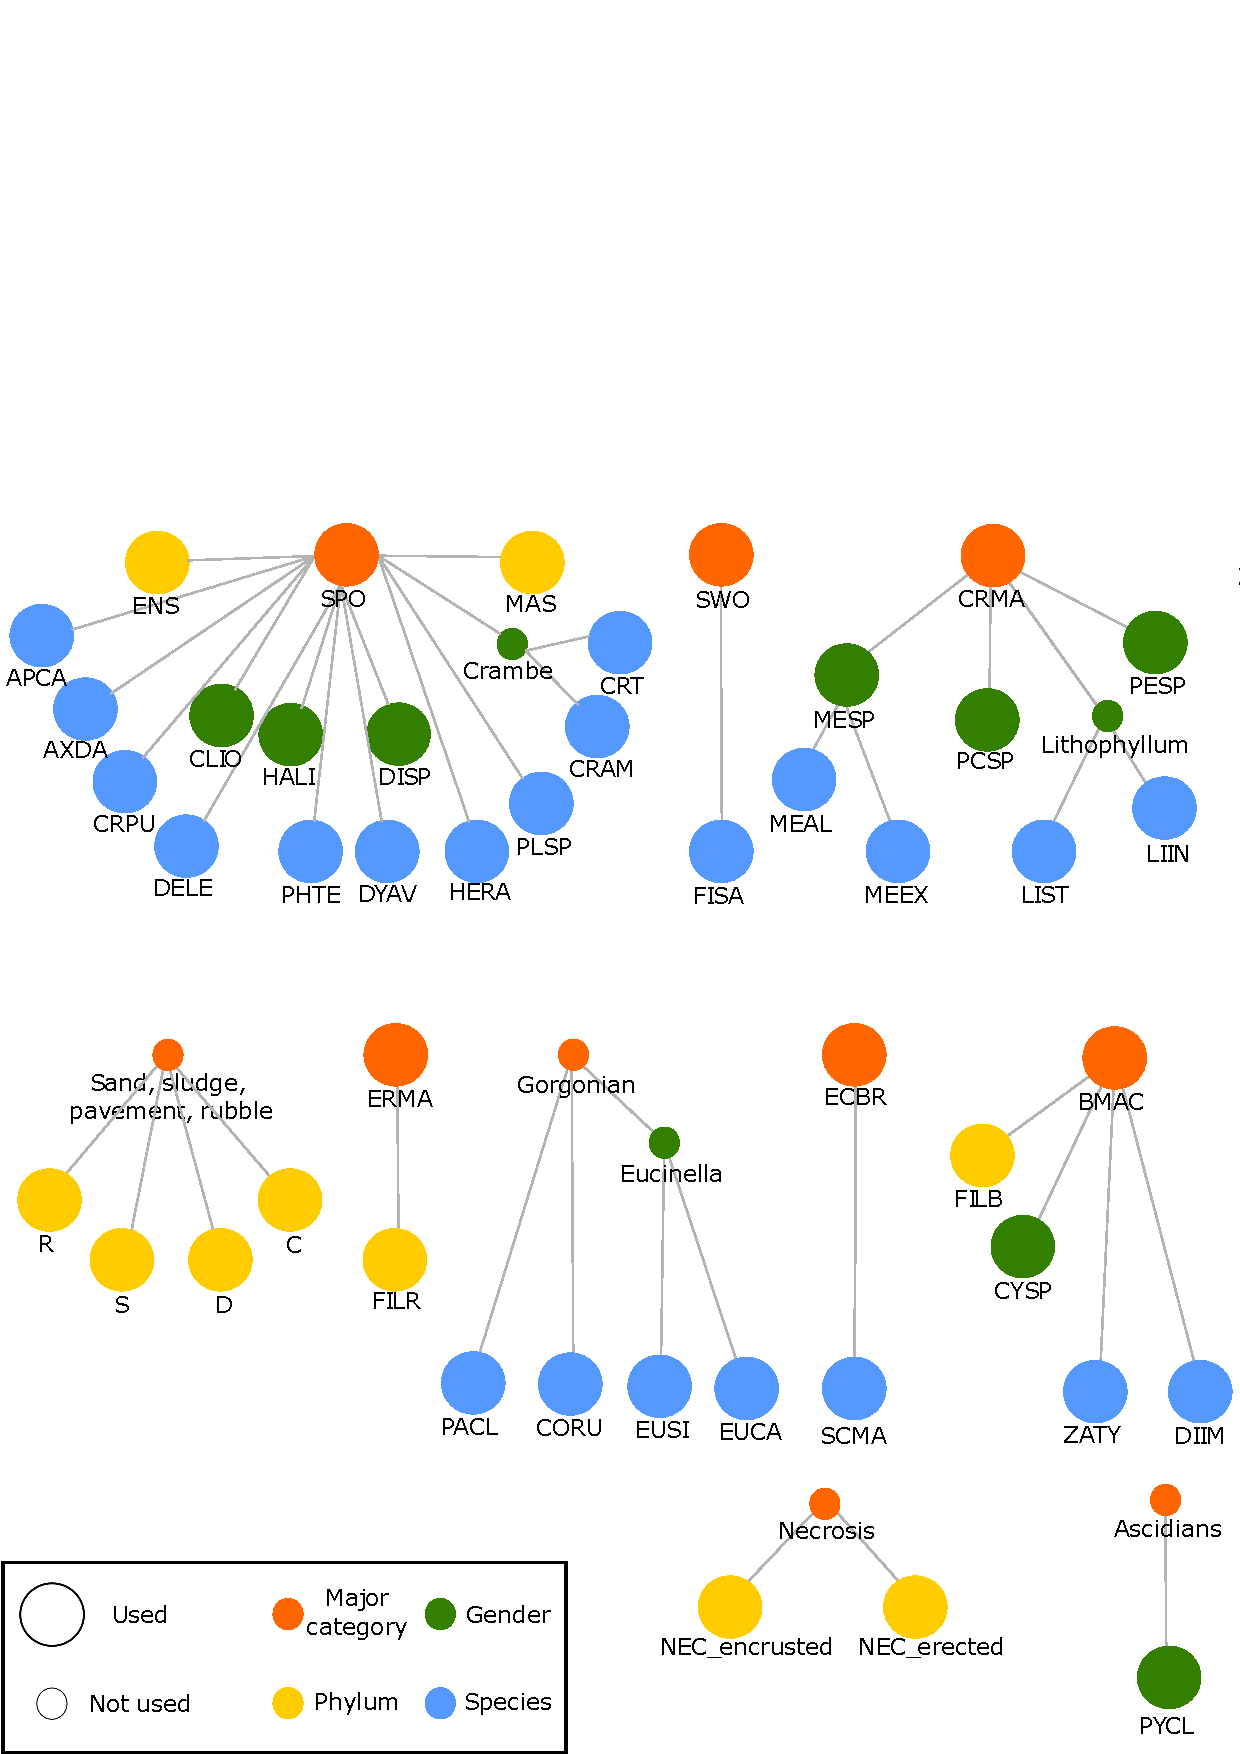
\includegraphics[width=\linewidth,keepaspectratio]{./3_chapitre1/Figure1.4}
		\caption[Classes of coralligenous taxa, hierarchically organised]{Classes of coralligenous taxa, hierarchically organised. Each network represents a major category (orange) linked to related phylums (yellow), genders (green) and species (blue). Smaller circles represent categories not subject to the original classification task and are written out in words. ADC = \textit{Adeonella calveti}; APCA = \textit{Aplysina cavernicola}; AXDA = \textit{Axinella damicornis}; BMAC = \textit{Brown macroalgae}; C = Crevice; CELL = \textit{Cellaria sp.}; CLIO = \textit{Cliona sp.}; CORU = \textit{Corallium rubrum}; CRAM = \textit{Crambe crambe}; CRMA = Encrusting red macroalgae; CRPU = \textit{Crella pulvinar}; CRSP = \textit{Crisia sp.}; CRT = \textit{Crambe tailliezi}; CYSP = \textit{Cystoseira sp.}; D = Sand; DELE = \textit{Dendroxea lenis}; DIIM = \textit{Dictyota implexa}; DISP = \textit{Dictyonella sp.}; DYAV = \textit{Dysidea avara}; ECBR = Encrusting bryozoan; ENS = Non identified encrusting sponge; ERBR = Erected bryozoan; ERMA = Erected red macroalgae; EUCA = \textit{Eunicella cavolini}; EUSI = \textit{Eunicella singularis}; FILB = Filamentous brown algae; FILG = Filamentous green algae; FILR = Filamentous red algae; FISA = \textit{Filograna} or \textit{Salmacina sp.}; FLPE = \textit{Flabellia petiolate}; GMAC = Green macroalgae; HALI = \textit{Haliclona sp.}; HATU = \textit{Halimeda tuna}; HERA = \textit{Hexadella racovitzai}; HY = Hydrozoa; LEPR = \textit{Leptopsammia pruvoti}; LIIN = \textit{Lithophyllum incrustans}; LIST = \textit{Lithophyllum stictaeforme}; MAS = Non identified massive sponge; MEAL = \textit{Mesophyllum alternans}; MEEX = \textit{Mesophyllum expansum}; MESP = \textit{Mesophyllum sp.}; MYT = \textit{Myriapora truncate}; NEC$\_$encrusted = Encrusted necrosis; NEC$\_$erected = Erected necrosis; PAAX = \textit{Parazoanthus axinellae}; PACL = \textit{Paramuricea clavata}; PACR = \textit{Palmophyllum crissum}; PCSP = Encrusting \textit{Peyssonnelia sp.}; PEF = \textit{Pentapora fascialis}; PESP = Erected \textit{Peyssonnelia sp.}; PHTE = \textit{Phorbas tenacior}; PLSP = \textit{Pleraplysilla spinifera}; PYCL = \textit{Pycnoclavella sp.}; R = Rubble; S = Sludge; SCMA = \textit{Schizomavella mamillata}; SPO = Sponges; SWO = Sedentary worms; VAMA = \textit{Valonia macrophysa}; ZATY = \textit{Zanardinia typus}.}
	\label{figure1.4}
\end{center}
\end{figure}

For instance, Mesophyllum alternans (MEAL) and Mesophyllum expansum (MEEX) are different species belonging to the same gender Mesophyllum sp (MESP), and Mesophyllum sp belongs to the major category Encrusting red macroalgae (CRMA). These classes also share a lot of visual characteristics, and it is the task of the algorithm to find the features common to one particular class which are not shared by specific subcategories. This requires an expert knowledge and is qualified as a fine-grained classification task \citep{akata_evaluation_2015}.

%%%%%%%%%%%%%%%%%%%%%%%%%%%%%%%%%%%%%%%%%%%%%%%%%%
%%% Figure 1.5: intra and inter-class variance %%%
%%%%%%%%%%%%%%%%%%%%%%%%%%%%%%%%%%%%%%%%%%%%%%%%%%
\begin{figure}[H]
	\begin{center}
	\includegraphics[width=0.8\linewidth,keepaspectratio]{./3_chapitre1/Figure1.5}
		\caption[Illustration of intra and inter-class variance]{Illustration of intra and inter-class variance. MEAL = Mesophyllum alternans; MEEX = Mesophyllum expansum; MESP = Mesophyllum sp.; CRMA = Encrusting red macroalgae.}
	\label{figure1.5}
\end{center}
\end{figure}

\section{Methodology}\label{chapitre1_4}

This study sought to design and train an algorithm based on deep CNN architectures, in order to identify a selection of coralligenous species or their broader taxonomical group, and to assess the biodiversity and ecological status of coralligenous reefs. We designed a custom methodology, drawing on state-of-the-art architectures and a large database of annotated photographic quadrats. More specifically, we performed the following analysis :

\begin{enumerate}
\item Assess human annotation error on a similar problem in order to establish a baseline performance;
\item Train simple CNNs on different patch sizes and build an ensemble network in order to improve performances with multi-scale prediction;
\item Train a LR on deeply learned features from intermediate layers to improve performances and calibrate the ensemble network;
\item Build a semi-automated tool based on the calibrated ensemble network, allowing to classify a dataset with a required minimum error risk;
\item Reduce the classification level of detail by grouping classes to higher taxonomical degrees (56 genders and 15 major categories), to build a customizable tool able to classify at different levels of details with corresponding accuracies.
\end{enumerate}

\subsection{Assessment of annotator reliability}\label{chapitre1_4.1}
We used the data from \citet{beijbom_towards_2015} (see \autoref{chapitre1_2.1}) to assess human annotator accuracy using F1-score (see section 5.2.1). For each point, the ground truth was defined as the first identification by the “host” expert. These results will be used to discuss our CNN classification performances.

\subsection{Ensemble network for multi-scale prediction}\label{chapitre1_4.2}
Different studies showed that in a patch-based classification context, multiple scales classification improved the final performances of the classifier \citep{beijbom_automated_2012, mahmood_coral_2016}. Indeed, many cases can challenge a patch-based classifier (small vs large individuals, point located on the edge between two classes…), and the integration of analyses made at different scales can help build a more robust and discriminative classifier. Therefore, we trained an ensemble of ResNet18s on four patch sizes (see \autoref{figure1.6}): \(224 \times 224\), the standard input sizes for most CNNs, \(128 \times 128\), \(96 \times 96\), and \(64 \times 64\) pixels. However, our methodology slightly differs from earlier works in two main aspects. Firstly, \citet{mahmood_coral_2016} resized the extracted patches to fix input dimensions as they used a pre-trained network. Conversely, we trained ResNet18s from scratch and consequently, input size was able to correspond to the size of the extracted patches. This avoids information loss which comes as a consequence of upscaling of small patches. Secondly, instead of implementing a max pooling set on the last convolutional layer \citep{mahmood_coral_2016}, our ensemble network uses the four outputs from the Global Average Pooling (GAP) layers, following the last convolutional block of the trained ResNet18. This ensures that more information is preserved and can be processed by a Multi-Layer Perceptron (MLP) and the concatenation results in a 2048 features vector. Our MLP was made up of three fully connected layers, of sizes 512 (fc512), 256 (fc256) and 61; the first two layers used ReLU activation, and the final layer a softmax, for classification.


\subsection{Logistic regression with deeply learned features}\label{chapitre1_4.3}
We trained LR models with different inputs, from the features learned by the deep learning model (output of the concatenation layer feeding the MLP; see Figure 6), to the more processed logits of the softmax layer:

\begin{itemize}
    \item Features from the concatenation of GAP outputs; 
    \item Features from the first layer of the MLP (fc512);
    \item Features from the second layer of the MLP (fc256);
    \item Logits of the softmax layer;
    \item Concatenation of the features of fc256 and the logits (see Figure 6). 
    
\end{itemize}

%%%%%%%%%%%%%%%%%%%%%%%%%%%%%%%%%%%%%%%%%%%%%%%%%%%%%
%%% Figure 1.6: Structure of the ensemble network %%%
%%%%%%%%%%%%%%%%%%%%%%%%%%%%%%%%%%%%%%%%%%%%%%%%%%%%%
\begin{figure}[H]
	\begin{center}
	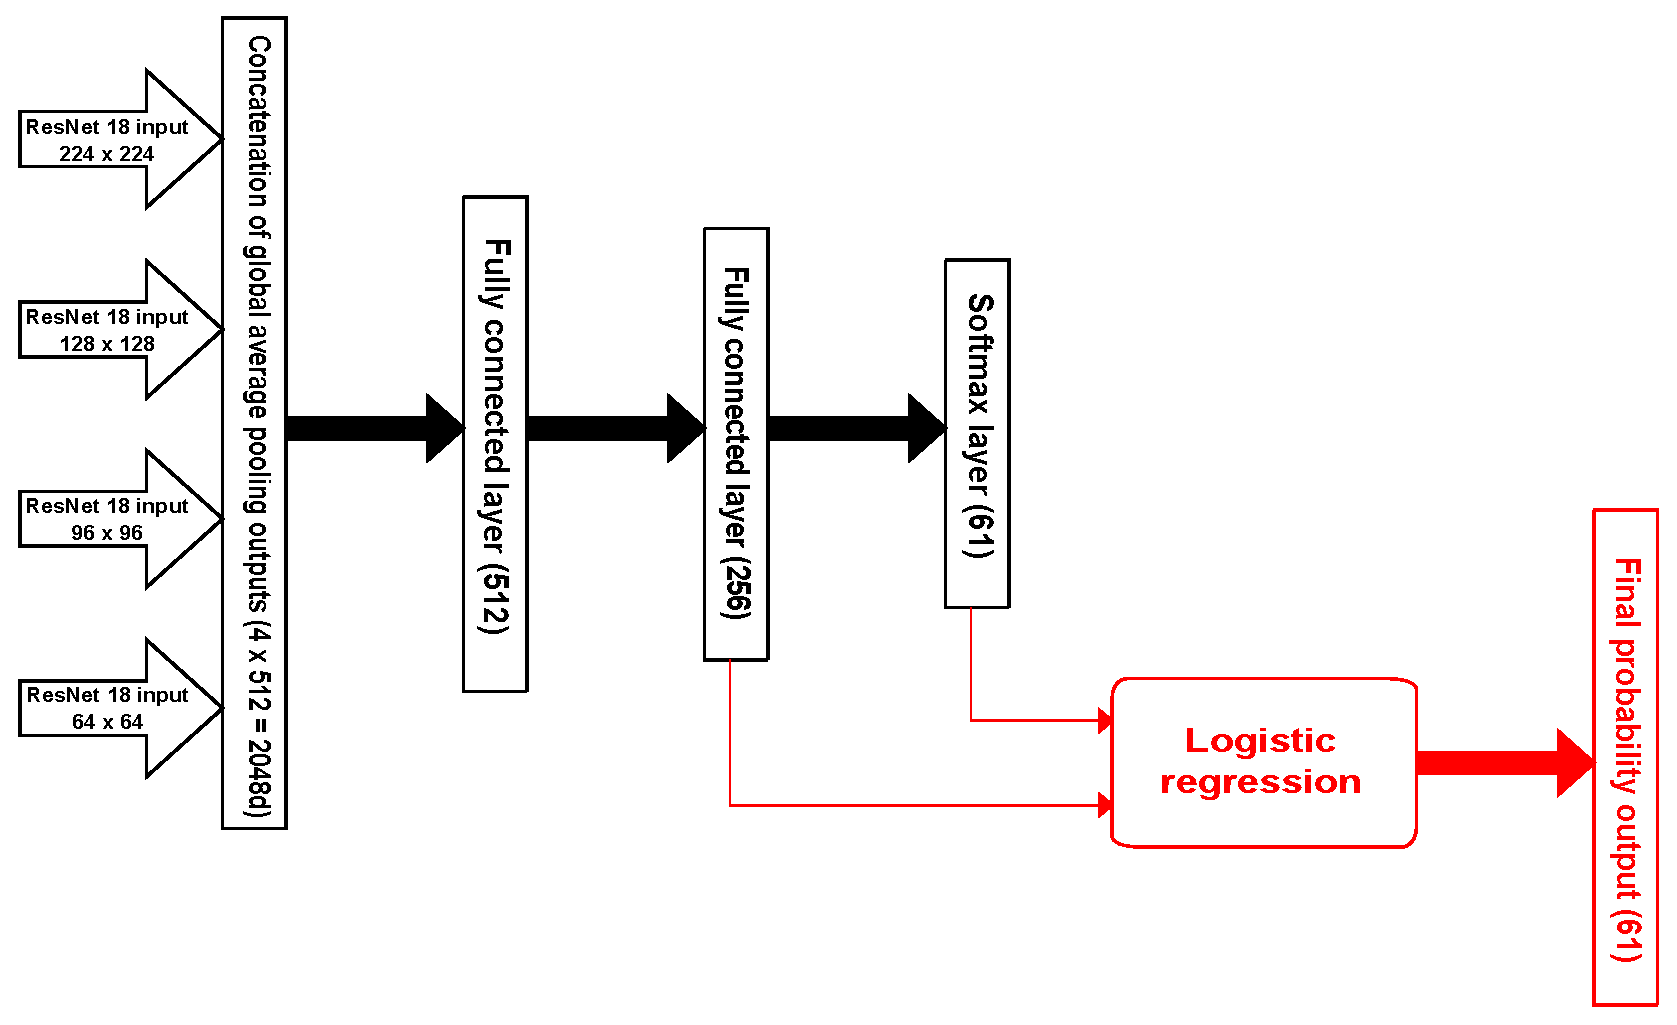
\includegraphics[width=\linewidth,keepaspectratio]{./3_chapitre1/Figure1.6}
		\caption[Structure of the ensemble network]{Structure of the ensemble network without (black) and with (red) machine learning prediction on deeply learned features (outputs of the two last layers of the MLP are concatenated and passed as input to a logistic regression). Features from global average pooling layer of four ResNet18s are fed to a MLP made of three fully connected layers of size: 512 and 256 with ReLU activation, and 61 with softmax for classification.}
	\label{figure1.6}
\end{center}
\end{figure}

\subsection{Semi-automated framework with selective classification}\label{chapitre1_4.4}
Selective classification, also called “reject option” \citep{herbei_classification_2006}, is a technique used to optimise classification performance. By training a classifier to decide whether or not a prediction is reliable, this technique reduces the error rate at the cost of a decrease in the classification rate, since the algorithm rejects certain samples which can later be manually labelled by an expert. This has been empirically investigated previously, in the case of image classification of marine habitats \citep{beijbom_automated_2012, beijbom_towards_2015}. Thresholding is a simple and fast method for mitigating a lack of performances in the classification task, in the event that the accuracy of human annotations in the dataset is lacking. Within a more theoretical framework, the use of selective classification with neural networks has previously been studied to find the best possible rejection rule \citep{geifman_selective_2017}. They called this risk-coverage approach “Selection with Guaranteed Risk” (SGR). For a given desired risk (i.e misclassification rate), the SGR maximises classification coverage while keeping the risk below the limit. 

Implementation of selective classification requires a good calibration of the network, i.e. the network should output a probability score equivalent to the empirical accuracy; for an output score of 0.8 for example, the network should predict the right class in 80 \% of the cases. However, a recent study showed that deep neural networks are not always well calibrated, and they tend to output over-confident prediction scores \citep{guo_calibration_2017}. Hyperparameters, such as depth, batch normalization, and weight decay, have been shown to influence calibration. Scaling the logits passed to the softmax function can also help calibrate the network.


\subsection{Categories merging: from coarse-to-fine biodiversity assessment}\label{chapitre1_4.5}
In order to provide different levels of analysis ranging from coarse to fine, and to enhance classification performances, we analysed the classification results at different taxonomic levels by grouping classes by gender or major category after classification with the 61-class network. As seen above, the relations between classes describe a complex and interconnected schema. Degrading the level of detail for the classification task was therefore expected to increase classification accuracy, as the different class levels were set according to a taxonomic hierarchy between original classes that share common visual characteristics. Level 1 corresponds to the original classification task (61 classes), level 2 corresponds to a classification at the gender level (54 classes; see Figure 4), and level 3 corresponds to the major category (15 classes). Furthermore, level 3 grouping describes a reduced number of classes which allowed us to have insight into class-wise performances and distribution.

\section{Experimental settings}\label{chapitre1_5}

\subsection{Training procedure}\label{chapitre1_5.1}
It has been previously established that on a similar case which involved patch-based coral classification, the ResNet152 architecture performed best \citep{king_comparison_2018}. However, this architecture is very deep and considers tens of millions of parameters. Consequently, we experimented on different, shallower CNNs which were modelled on this architecture (ResNet18 and ResNet50). Unlike many previous studies which used transfer learning \citep{king_comparison_2018, mahmood_coral_2016, mahmood_deep_2017}, we trained our CNNs from scratch. Different ResNet18s were trained with batch normalization and ReLU activation taking place before the convolution layer, as this has been proven to improve generalization \citep{he_identity_2016}. We trained these CNNs using Adam optimiser, with a learning rate of $10^{-3}$ and other parameters set to their defaults, in accordance with the original study \citep{kingma_adam:_2014}. Data was fed iteratively in batches of 512, for patches of dimensions \(64 \times 64\), \(96 \times 96\) and \(128 \times 128\) pixels. Batches of 200 were used for patch size \(224 \times 224\) due to computational limitations. A ResNet50 was also trained under the same conditions, with patch size \(128 \times 128\) and batch size 128, once again due to computational limitations. In order to better compare the networks, a ResNet18 was also trained with same conditions as the ResNet50. The ensemble network was built on four ResNet18s (see \autoref{figure1.6}) which were independently trained on the four patch sizes. The ensemble was then fine-tuned: we used a batch size of 128, froze the weights from the ResNet18s, and used the same optimiser and parameters as mentioned above. Data augmentation on all patches was performed for all trained networks, in order to compensate for the high class imbalance and allow a better generalization. We applied random rotations between 0 and 180 degrees, brightness scaling between 0.4 and 1.6, and horizontal / vertical flipping to all patches on the fly as data was fed to the networks. Trainings lasted at least 100 epochs and were stopped when validation accuracy did not improve for 25 epochs.

A ResNet152 was used as the baseline for classification performance. This network was initially programmed using pre-trained weights lifted from the ImageNet challenge. The top fully-connected layer was replaced with a layer using ReLU activation, followed by a dropout layer and a softmax layer, with outputs corresponding to the number of classes (here 61). Firstly, the top layer was trained alone; using features extracted from the convolutional layers, a Stochastic Gradient Descent (SGD) with a learning rate of $10^{-3}$, and weight decay rate set to $5\times10^{-4}$. The whole network was then trained with SGD; learning rate$10^{-4}$ and weight decay $10^{-6}$. Patches of \(224 \times 224\) were fed in batches of 16. Training was performed over 50 epochs until loss on the validation set stopped decreasing.

The deeply learned features and the different layer outputs of the training, validation, and test sets were extracted in advance. LRs were trained and optimised using the grid search tool implemented in scikit-learn \footnote{Scikit-learn v 0.20.2} on the validation set.

SGR was applied at risk levels ranging from 5 to 30 \% and resultant thresholds. Coverages and bounds for the coverage were assessed together with top-5 accuracy on the unclassified part of the dataset. SGR was trained on the validation set and applied to the training and test set with the aforementioned risk levels to assess the corresponding coverages.

All architectures were implemented in Python 3.6 using the Keras \footnote{Keras v 2.2.4} library and Tensorflow \footnote{Tensorflow v 1.12.0} backend. All training and testing processes were performed on a Windows 10 workstation with 64 bits OS, 128 Gb RAM, \(2 \times\)NVidia GeForce GTX 1080 Ti 11 Gb memory and 12 cores CPU 2.9 GHz.

\subsection{Evaluation metrics}\label{chapitre1_5.2}

\subsubsection{Classification performances}\label{chapitre1_5.2.1}

The performances of the networks were assessed with the precision, recall and F1-score. At training, validation and testing time; precision, recall and F1-score were calculated as follows:

\begin{equation}
\text{F1-score}=2\times\frac{\text{Precision}\times\text{Recall}}{\text{Precision}+\text{Recall}}
\end{equation}

With:

\begin{equation}
\text{Precision}=\frac{\text{True Positive}}{\text{True Positive}+\text{False Positive}}
\end{equation}

\begin{equation}
\text{Recall}=\frac{\text{True Positive}}{\text{True Positive}+\text{False Negative}}
\end{equation}

F1 ranges from 0 to 1, 1 being a perfect classifier.

The three metrics were computed at both micro and macro levels. Micro-F1, precision, and recall computed the statistics across all classes, given their distribution on the whole dataset, while macro statistics placed equal weight on all classes, meaning that class-wise differences in performance more greatly impacted the scores. This rendered micro-recall equivalent to the overall top-1 accuracy of the models (these two terms will be used interchangeably).

\subsubsection{Calibration of the networks}\label{chapitre1_5.2.2}

After training, network calibration was evaluated on the validation set for the best ResNet18, the baseline ResNet152, and the ensemble network with and without LR. Predictions were grouped in M bins of same size for the computation of accuracy according to the following equation \citep{guo_calibration_2017}:

\begin{equation}
	acc(B_m)=\frac{1}{|B_m|}\sum_{i\in B_m}\textbf{1}(\hat{y}_i=y_i)
\end{equation}

Where $B_m$ is the set of indices of the instances composing bin $m$, $\hat{y}_i$ the predicted class of instance $i$ and $y_i$ its true class. Average confidence for $B_m$ is then given by :

\begin{equation}
conf(B_m)=\frac{1}{|B_m|}\sum_{i\in B_m}\hat{p}_i
\end{equation}

With $\hat{p}_i$ the outputted probability corresponding to the class $\hat{y}_i$. On top of the diagrams, Estimated Calibration Error (ECE) was calculated for the models considered with the following equation.

\begin{equation}
\text{ECE}=\sum_{m=1}^{M}\frac{|B_m|}{n}|acc(B_m)-conf(B_m)|
\end{equation}

With $n$ the total number of samples in the dataset.


\subsubsection{Coralligenous ecological status and biodiversity assessment}\label{chapitre1_5.2.3}
Coralligenous health is typically assessed using the Coralligenous Assemblage Index (CAI) \citep{deter_preliminary_2012}. This is based on the prevalence of bryozoans, major builders and sludge in an assemblage. The CAI is calculated as follows:

\begin{equation}
\text{CAI\textsubscript{i}}=\frac{1}{3}\times(\frac{1-sludge_i}{1-\min_{i}sludge_i}+\frac{majbuilders_i}{\max_{i}majbuilders_i}+\frac{bryozoans_i}{\max_{i}bryozoans_i})
\end{equation}

With \textit{sludge\textsubscript{i}}, \textit{majbuilders\textsubscript{i}} and \textit{bryozoans\textsubscript{i}}, the covering percentage of sludge, major builders (13 classes out of the 61) and bryozoans (8 classes out of the 61) respectively. Minimum and maximum values of these percentages are calculated over all study sites. CAI is classically measured on 30 quadrats, 64 points per quadrat, for a total of 1920 annotated points.

Biodiversity indices are numerous. This includes simpler indices, such as species richness which refers to the number of observed species, and more integrated indices which take abundance into account in order to attribute more or less weight to common or rare species \citep{magurran_measuring_2004}. One commonly used index is the Shannon index:

\begin{equation}
	S_j=-\sum_{i}p_{ij} log(p_{ij})
\end{equation}

With \textit{p\textsubscript{ij}} the prevalence of species \textit{i} among site \textit{j}.

Both indices were modelled by randomly selecting 10 000 sets of 1 920 instances from the test set of 31 467 instances). For each set of 1 920, proportions of sludge / bryozoans / major builders, CAI and Shannon index were calculated on the ground truth and the automatic labels. Pearson correlations were used to analyse the fit between true and modelled indices.

\section{Results}\label{chapitre1_6}

\subsection{Human error}\label{chapitre1_6.1}
The assessment of human annotator reliability on the dataset presented in section 2.1 showed variable performances across the expert panel (see \autoref{table1.1}). All metrics were significantly higher for the hosts (who performed the ground truth annotation) than visitors, and micro-F1 was higher than macro-F1 for both the hosts and visitors.


%%%%%%%%%%%%%%%%%%%%%%%%%%%%%%%
%%% Table 1.1: Human error  %%%
%%%%%%%%%%%%%%%%%%%%%%%%%%%%%%%
\begin{table}[htbp]
  \centering
  \normalsize
 % \raggedright
  \caption[Classification accuracy of hosts (n = 4) and visitors (n = 20) on the Moorea dataset]{Classification accuracy of hosts (n = 4) and visitors (n = 20) on the Moorea dataset (Beijbom et al., 2012). \textit{Values are given in mean percentage ± standard deviation.}}
  \label{table1.1}
    \begin{tabular}{*{4}{c}}
        \toprule
        \textbf{Subject} & \textbf{Macro-F1} & \textbf{Top-1 accuracy} & \textbf{Micro-F1} \\ \midrule
        hosts            & 74.86 ± 3.63      & 79.21 ± 2.35            & 80.32 ± 2.32      \\
        visitors         & 59.4 ± 4.15       & 64.98 ± 6.31            & 68.31 ± 4.64      \\ \bottomrule
    \end{tabular}
\end{table}

\subsection{CNN performances}\label{chapitre1_6.2}

\subsubsection{Simple CNNs and ensemble network}\label{chapitre1_6.2.1}
All validation performances consistently increased with the patch size up to 224 × 224, which achieved 65.94 micro-F1 (see \autoref{table1.2}). As for training curves, the gap between patch size performances tended to decrease quickly. It is worth emphasizing that macro-F1 (with all classes weighted equally) was consistently lower than micro-F1 (all classes weighted according to their proportion in the dataset).

%%%%%%%%%%%%%%%%%%%%%%%%%%%%%%%%%%%%%%%%%
%%% Table 1.2: Performances ResNet18  %%%
%%%%%%%%%%%%%%%%%%%%%%%%%%%%%%%%%%%%%%%%%
\begin{table}[htbp]
  \centering
  \normalsize
  %\raggedright
  \caption{Performances of the ResNet18 on the validation and test sets for different input sizes (patch size).}
  \label{table1.2}
  %\scalebox{0.95}[0.95]{
    \begin{tabular}{*{2}{c}|*{3}{c}|*{3}{c}}
        \toprule
        \multicolumn{2}{c}{\textbf{}}             & \multicolumn{3}{c}{\textbf{Validation set}}                     & \multicolumn{3}{c}{\textbf{Test set}}                           \\ 
        \midrule
        \textbf{Patch Size} & \makecell{\textbf{Batch} \\ \textbf{size}} & \textbf{Macro-F1} & \makecell{\textbf{Top-1} \\ \textbf{accuracy}} & \textbf{Micro-F1} & \textbf{Macro-F1} & \makecell{\textbf{Top-1} \\ \textbf{accuracy}} & \textbf{Micro-F1} \\ \midrule
        64 × 64             & 512                 & 40.29             & 54.43                   & 55.07             & 46.50             & 60.64                   & 60.17             \\
        96 × 96             & 512                 & 51.21             & 63.97                   & 63.73             & 51.75             & 63.82                   & 63.57             \\
        128 × 128           & 512                 & 54.28             & 65.99                   & 65.85             & 54.08             & 65.77                   & 65.54             \\
        224 × 224           & 200                 & 54.93             & 66.70                   & 66.44             & 53.93             & 66.30                   & 65.94             \\ \bottomrule
    \end{tabular}
    %}
\end{table}

The ResNet18 and ResNet50 trained with the same hyperparameters  (see \autoref{table1.3}, ResNet50-128 and ResNet18-128) performed roughly equally on validation and test sets, with ResNet18-128 achieving a micro-F1 of 63.44 and ResNet50 63.89 on the test set. However, an epoch for the ResNet50 took about three times longer than ResNet18. The ResNet50 did not outperform the previously trained ResNet18 with patch size 128 and batch size 512 (see \autoref{table1.2}). The deeper architecture of the ResNet50 made it impossible to train with a batch size of 512.

%%%%%%%%%%%%%%%%%%%%%%%%%%%%%%%%%%%%%%%%%%%%%%%%%%%%%
%%% Table 1.3: Performances of different ResNet   %%%
%%%%%%%%%%%%%%%%%%%%%%%%%%%%%%%%%%%%%%%%%%%%%%%%%%%%%
\begin{table}[htbp]
  \centering
  \normalsize
 % \raggedright
  \caption[Performances of different ResNet architectures on validation and test sets]{Performances of different ResNet architectures on validation and test sets. ResNetX-Y is written so that X indicates the network’s depth and Y the input size.}
  \label{table1.3}
    \begin{tabular}{*{2}{c}|*{3}{c}|*{3}{c}}
        \toprule
        \multicolumn{2}{c}{\textbf{}}                      & \multicolumn{3}{c}{\textbf{Validation set}}                     & \multicolumn{3}{c}{\textbf{Test set}}                           \\ \midrule
        \textbf{Network} & \makecell{\textbf{Batch} \\ \textbf{size}} & \textbf{Macro-F1} & \makecell{\textbf{Top-1} \\ \textbf{accuracy}} & \textbf{Micro-F1} & \textbf{Macro-F1} & \makecell{\textbf{Top-1} \\ \textbf{accuracy}} & \textbf{Micro-F1} \\
        \midrule
        ResNet152-224                & 16                  & 37.45             & 62.38                   & 60.46             & 38.26             & 61.71                   & 60.09             \\
        ResNet50-128                 & 128                 & 52.04             & 64.07                   & 63.85             & 52.27             & 64.35                   & 63.89             \\
        ResNet18-128                 & 128                 & 51.40             & 63.90                   & 63.88             & 51.62             & 63.60                   & 63.44             \\
        ResNet18-224                 & 200                 & 54.93             & 66.70                   & 66.44             & 53.93             & 66.30                   & 65.94             \\
        Ensemble                     & 128                 & \textbf{60.56}    & \textbf{70.60}          & \textbf{70.35}    & \textbf{60.38}    & \textbf{70.54}          & \textbf{70.37}    \\ \bottomrule
    \end{tabular}
\end{table}

The ensemble network performed better than any previous CNN on validation and test sets (70.35 and 70.37 micro-F1, respectively), and outperformed both the best, single ResNet18 (65.94, see \autoref{table1.2}) and the baseline ResNet152 (60.09, see \autoref{table1.3}). The latter performed worse than any other network considered here for all metrics, with macro-F1 (37.45 and 38.26 on validation and test sets, respectively) lower than micro scores (micro-F1 of 60.46 and 60.09). With the sole exception of CNN for patch size 64 × 64, validation and test performances were very similar for all trained models, and macro metrics were consistently lower than micro metrics.

\subsubsection{Ensemble network with logistic regression}\label{chapitre1_6.2.2}
LRs were trained using l2 penalty and multinomial loss, with the following parameters defined with grid search on the validation set: C = 0.01 and saga solver . Results were compared with each other and with the ensemble alone (see \autoref{table1.4}).

%%%%%%%%%%%%%%%%%%%%%%%%%%%%%%%%%%%%%%%%%%%%%%%%%%%%%%%%
%%% Table 1.4: Performances of logistic regression   %%%
%%%%%%%%%%%%%%%%%%%%%%%%%%%%%%%%%%%%%%%%%%%%%%%%%%%%%%%%
\begin{table}[htbp]
    \centering
      \caption[Performances of logistic regression applied to different layers of the ensemble network, on validation and test sets]{Performances of logistic regression applied to different layers of the ensemble network, on validation and test sets. None: ensemble alone, logits: features of the last layer before softmax, fc256: features from the penultimate layer; fc512: features from the first layer of the Multi-Layer Perceptron (MLP); GAP: features from the concatenation of global average pooling before the MLP.}
      \label{table1.4}
    \begin{tabular}{*{1}{c}|*{3}{c}|*{3}{c}}
    	\toprule
    	\textbf{} & \multicolumn{3}{c}{\textbf{Validation set}} & \multicolumn{3}{c}{\textbf{Testing set}}\\
    	\midrule
    	\textbf{Features} & \textbf{Macro-F1} & \textbf{Top-1 accuracy} & \textbf{Micro-F1} & \textbf{Macro-F1} & \textbf{Top-1 accuracy} & \textbf{Micro-F1}\\
    	\midrule%[0.05cm] % épaisseur du trait
    	None & 60.56 & 70.60 & 70.35 & 60.38 & 70.54 & 70.37\\
    	logits & 61.93 & 72.23 & 71.81 & 61.69 & 71.91 & 71.50\\
    	fc256 & \textbf{63.92} & 72.62 & 72.28 & 62,69 & 72.41 & 72.02\\
    	fc512 & 16.31 & 55.09 & 53.23 & 8.55 & 44.12 & 42.37\\
    	GAP & 10.12 & 46.67 & 45.19 & 6.70 & 38.64 & 37.31\\
    	combined & 63.74 & \textbf{72.69} & \textbf{72.32} & \textbf{63.91} & \textbf{72.59} & \textbf{72.20}\\
    	\bottomrule
    \end{tabular}
\end{table}

The LR on the logits and features from the penultimate layer (fc256) resulted in an improvement in both macro and micro metrics scores, compared with the ensemble network alone (see “None”, \autoref{table1.4}). On the test set, micro-F1 increased from 70.37 to 71.50 using logits, and 72.02 using the penultimate layer, while macro-F1 increased from 60.38 to 61.69 and 62.69 respectively. The use of both layers’ features (see “fc256 + logits”, \autoref{table1.4}) resulted in a marginal improvement (63.91 for macro-F1 and 72.20 for micro-F1 on the test set). Using features from the first layer of the MLP (fc512), or the concatenation of global average pooling outputs, resulted in consistent degradation of all metrics on the validation set, and results were even worse for the test set. Using the best model, out of the 61 classes, 11 showed an accuracy > 80 \% (\textit{“Aplysina cavernicola”}, “Crevice”, \textit{“Corallium rubrum”}, \textit{“Crambe tailliezi”}, \textit{“Eunicella cavolini”}, \textit{“Hexadella racovitzai”}, \textit{“Leptopsammia pruvoti”}, \textit{“Mesophyllum alternans”}, \textit{“Parazoanthus axinellae”}, \textit{“Paramuricea clavata”}, \textit{“Erected Peyssonnelia sp.”}) and 12 had an accuracy comprised between 70 \% and 80 \% (“Sand”, \textit{“Eunicella singularis”}, “Filamentous green algae”, “Filamentous red algae”, \textit{”Flabellia petiolata”}, \textit{“Haliclona sp.”}, \textit{“Halimeda tuna”}, \textit{“Palmophyllum crassum”}, \textit{“Encrusting Peyssonnelia sp.”}, \textit{“Pentapora fascialis”}, \textit{“Phorbas tenacior”}, \textit{“Pleraplysilla spinifera”}).

\subsection{Post-processing}\label{chapitre1_6.3}

\subsubsection{Semi-automated classification}\label{chapitre1_6.3.1}
Reliability diagrams –which plot confidence against accuracy – were plotted for the baseline ResNet152, the best ResNet18, and the ensemble network with and without LR (see \autoref{figure1.7}). The red line shows a theoretical, perfect calibration (y = x).

%%%%%%%%%%%%%%%%%%%%%%%%%%%%%%%%%%%%%%%%%%%%%%%%%%%%%%%%%%%%%%%%%%
%%% Figure 1.7: Reliability diagrams of the different networks %%%
%%%%%%%%%%%%%%%%%%%%%%%%%%%%%%%%%%%%%%%%%%%%%%%%%%%%%%%%%%%%%%%%%%
\begin{figure}[H]
	\begin{center}
	\includegraphics[width=\linewidth,keepaspectratio]{./3_chapitre1/Figure1.7}
		\caption[Reliability diagrams of the different networks]{Reliability diagrams of the different networks. The red curve corresponds to a perfect calibration (y = x). ECE = Estimated Calibration Error; ResNet152 = RestNet152 with patch size 224 × 224 and batch size 16; RestNet18 = RestNet18 with patch size \(224 \times 224\) and batch size 200; Ensemble Network = ensemble of the four ResNet18 with the four patch sizes (\(64 \times 64\), \(96 \times 96\), \(128 \times 128\) and \(224 \times 224\) pixels); Ensemble Network + LR = ensemble network with the logistic regression on the results of both the penultimate fully connected layer (fc256) and the softmax layer.}
	\label{figure1.7}
\end{center}
\end{figure}

The ResNet152 showed the highest ECE with 6.21 \%, while the best single ResNet18 (patch size 224 and batch size 200) achieved 4.01 \%. The ensemble network had an ECE of 4.40 \% without LR. The best score was achieved by the ensemble network with LR applied to the logits and the penultimate layer, which displayed an ECE of 3.60 \%.

\medskip

The results, recorded after the SGR algorithm was applied for selective classification on the best ensemble network with LR, are summarised in \autoref{table1.5}. A top-1 accuracy of 85.65 \% (risk = 14.35 \%) was achieved when covering 67.48 \% of the test set, and 91.30 \% accuracy (risk = 8.70 \%) could be obtained when classifying more than 50 \% of the data. Top-5 accuracy on the uncovered part of the data was consistently between 80 and 95 \%.

%%%%%%%%%%%%%%%%%%%%%%%%%%%%%%%%%%%%%%%%%%%%%%%%%%%%%%%%
%%% Table 1.5: Performances of logistic regression   %%%
%%%%%%%%%%%%%%%%%%%%%%%%%%%%%%%%%%%%%%%%%%%%%%%%%%%%%%%%
\begin{table}[htbp]
  \centering
  \normalsize
 % \raggedright
  \caption[Application of the Selection with Guaranteed Risk algorithm on the validation set for training and results on the test set]{Application of the Selection with Guaranteed Risk algorithm on the validation set for training and results on the test set. Top-5 uncovered = top-5 accuracy for the rejected part of the test set. All numbers are expressed in \%.}
  \label{table1.5}
    \begin{tabular}{@{}cccccc@{}}
        \toprule
        \textbf{Desired risk} & \textbf{Train-risk} & \textbf{Train-coverage} & \textbf{Test-risk} & \textbf{Test-coverage} & \textbf{Top-5 uncovered} \\ \midrule
        5.00                  & 4.25                & 33.98                   & 4.20               & 33.72                  & 94.16                    \\
        10.00                 & 9.15                & 52.12                   & 8.70               & 51.90                  & 92.71                    \\
        15.00                 & 14.11               & 67.59                   & 14.35              & 67.48                  & 91.06                    \\
        20.00                 & 19.09               & 80.47                   & 19.26              & 80.62                  & 88.16                    \\
        25.00                 & 24.08               & 92.97                   & 24.24              & 93.17                  & 81.75                    \\
        30.00                 & 27.30               & 100.00                  & 27.40              & 100.00                 & -                        \\ \bottomrule
    \end{tabular}
\end{table}

\subsubsection{Categories merging}\label{chapitre1_6.3.2}
Post-classification merging of the predicted classes, according to the taxonomic hierarchy, resulted in the consistent augmentation of performances (see \autoref{table1.6}). Gender grouping (level 2) led to a moderate increase of top-1 accuracy (75.91 \% vs 72.59 \% on the test set) and a small decrease in the total number of classes, from 61 to 56. Merging classes according to their major category (level 3) resulted in a gain of 11.88 points on the test set. The task was then reduced to discriminate between 15 classes, and results were then on par with the human accuracy tested on a 20 class task as recorded in Table 1 (72.88 macro-F1 and 84.29 micro-F1 on the test set versus 74.86 macro-F1 and 80.32 micro-F1 for host annotators on the human evaluation dataset).

%%%%%%%%%%%%%%%%%%%%%%%%%%%%%%%%%%%%%%%%%%%%%%%%%%%%%%%%
%%% Table 1.6: Performances of logistic regression   %%%
%%%%%%%%%%%%%%%%%%%%%%%%%%%%%%%%%%%%%%%%%%%%%%%%%%%%%%%%
\begin{table}[htbp]
  \centering
  \normalsize
 % \raggedright
  \caption[Results for coarse-to-fine categories merging according to taxonomic hierarchy]{Results for coarse-to-fine categories merging according to taxonomic hierarchy. Level 1 = original classes (61); level 2 = gender level (56); level 3 = major category level (15).}
  \label{table1.6}
  \begin{tabular}{*{2}{c}|*{3}{c}|*{3}{c}}
        \toprule
        \multicolumn{2}{c}{\textbf{}}               & \multicolumn{3}{c}{\textbf{Validation set}}                     & \multicolumn{3}{c}{\textbf{Test set}}                           \\ \midrule
        \textbf{Model} & \makecell{\textbf{Number} \\ \textbf{of classes}} & \textbf{Macro-F1} & \makecell{\textbf{Top-1} \\ \textbf{accuracy}} & \textbf{Micro-F1} & \textbf{Macro-F1} & \makecell{\textbf{Top-1} \\ \textbf{accuracy}} & \textbf{Micro-F1} \\
        \midrule
        Level 1        & 61                         & 63.74             & 72.69                   & 72.32             & 63.91             & 72.59                   & 72.20             \\
        Level 2        & 56                         & 64.86             & 75.98                   & 75.53             & 64.76             & 75.91                   & 75.63             \\
        Level 3        & 15                         & 71.75             & 84.40                   & 84.21             & 72.88             & 84.47                   & 84.29             \\ \bottomrule
    \end{tabular}
\end{table}

Level 3 merging offers an easy insight into the class-wise performance of the classification process (see \autoref{figure1.8}). Out of the 15 classes, three tended to be misclassified; “encrusting bryozoan” tended to be misclassified as “encrusting red macroalgae” (17 \%) and “sponge” (17 \%); “Hydroid” was often mistaken for “brown macroalgae” (19 \%) or “sludge, pavement, rubble, sand” (15 \%); and “sedentary worms” were most often misclassified as “encrusting red macroalgae” (16 \%) or “sludge, pavement, rubble, sand” (15 \%). Overall, four classes were responsible for most of the confusion: “brown macroalgae”, “encrusting red macroalgae”, “sponge”, and “sludge, pavement, rubble, sand”. On the other hand, seven classes tended to be well classified (> 80 \% accuracy): “encrusting red macroalgae” (92 \%), “gorgonian” (91 \%), “green macroalgae” (85 \%), “scleractinia” (87 \%), “sponge” (84 \%), “zoantharia” (89 \%) and “sludge, pavement, rubble, sand” (83 \%).

%%%%%%%%%%%%%%%%%%%%%%%%%%%%%%%%%%%%%%%%%%%%%%%%%%%%%%%%%%%%%%%%%%%%%%%%%%%%
%%% Figure 1.8: Confusion matrix of the output from the ensemble network %%%
%%%%%%%%%%%%%%%%%%%%%%%%%%%%%%%%%%%%%%%%%%%%%%%%%%%%%%%%%%%%%%%%%%%%%%%%%%%%
\begin{figure}[H]
	\begin{center}
	\includegraphics[width=\linewidth,keepaspectratio]{./3_chapitre1/Figure1.8}
		\caption[Confusion matrix of the output from the ensemble network with logistic regression on the test set]{Confusion matrix of the output from the ensemble network with logistic regression on the test set. The 61 original classes were merged to their major category (15 classes). Numbers represent ground truth repartition in predicted classes (\%).}
	\label{figure1.8}
\end{center}
\end{figure}

\newpage

\subsection{Ecological indicators prediction}\label{chapitre1_6.4}
Predicted sludge and bryozoans were correlated moderately well with the ground truth (see \autoref{figure1.9}; pearson correlation: 0.54 and 0.61, respectively), but predicted and observed major builders showed higher correlation (pearson correlation: 0.82).

%%%%%%%%%%%%%%%%%%%%%%%%%%%%%%%%%%%%%%%%%%%%%%%%%%%%%%%%
%%% Figure 1.9: sludge, bryozoans and major builders %%%
%%%%%%%%%%%%%%%%%%%%%%%%%%%%%%%%%%%%%%%%%%%%%%%%%%%%%%%%
\begin{figure}[H]
	\begin{center}
	\includegraphics[width=\linewidth,keepaspectratio]{./3_chapitre1/Figure1.9}
		\caption[Predicted vs observed percentages of sludge, bryozoans and major builders]{Predicted vs observed percentages of sludge, bryozoans and major builders. Pearson correlations: Sludge = 0.54, Bryozoans = 0.61, Major builders = 0.82.}
	\label{figure1.9}
\end{center}
\end{figure}

Predicted CAI was moderately correlated with the ground truth (see \autoref{figure1.10}; pearson correlation: 0.61), but predicted and observed Shannon indices showed higher correlation (pearson correlation: 0.74).

%%%%%%%%%%%%%%%%%%%%%%%%%%%%%%%%%%%%%%%%%%%%%%%%%%%%%%%%%%%%%%%%%%%%%
%%% Figure 1.10: Coralligenous Assemblage Index and Shannon Index %%%
%%%%%%%%%%%%%%%%%%%%%%%%%%%%%%%%%%%%%%%%%%%%%%%%%%%%%%%%%%%%%%%%%%%%%
\begin{figure}[H]
	\begin{center}
	\includegraphics[width=0.7\linewidth,keepaspectratio]{./3_chapitre1/Figure1.10}
		\caption[Predicted vs observed Coralligenous Assemblage Index and Shannon Index]{Predicted vs observed Coralligenous Assemblage Index and Shannon Index. Pearson correlations: CAI = 0.61, Shannon Index = 0.74.}
	\label{figure1.10}
\end{center}
\end{figure}

\newpage

\section{Discussion}\label{chapitre1_7}

\subsection{Patch size influence}\label{chapitre1_7.1}
Although our dataset was large enough to train a CNN from scratch, it was limited to punctual annotations (at the pixel level) of photo quadrats, therefore it required patch-wise classification. The patch size was crucial (see \autoref{table1.2}), as it reflects a trade-off between local and contextual information. If the patch size is too small, it contains insufficient information and most probably fails to capture whole individuals; if it is too large, the context scrambles the signature of the central information, confusing the algorithm. The patch size \(64 \times 64\) pixels performed the worst out of all the metrics; the large differences between validation and test performances was indicative of its poor capacity for generalization. A patch size of \(224 \times 224\) gave the highest micro-F1 on the test set (65.94). This patch size included enough contextual noise to regularize overfitting, and it enabled better generalization. While the single RestNet18 based on the patch size \(224 \times 224\) obtained the best accuracy, our ensemble network, which was based on the four tested patch sizes and followed the feature extraction scheme of the local-SPP \citep{mahmood_coral_2016}, improved classification performances by 4.43 points (see \autoref{table1.3}). The biggest difference between our network and the original version of the local-SPP lies in the fact that we concatenated the four 512-dimension feature vectors, instead of the max-pooling layer, which enabled the information contributed by each patch size to be processed by the consecutive MLP without loss.

\subsection{Tuning the architecture}\label{chapitre1_7.2}
The training procedure of ResNet18, notably the batch size parameter, had a great impact on classification performance. This was indicated by the difference in micro-F1 values produced by a ResNet18 trained with batch size 128 (63.44; see \autoref{table1.3}) and a ResNet18 train with batch size 512 (65.54; see \autoref{table1.2}). These results provide a different perspective than the conclusions drawn by previous studies \citep{masters_revisiting_2018, mishkin_systematic_2016} where the use of small or even mini-batches enhanced performances. This could be explained by the high imbalance between classes and the fine-grained nature of the classification task. Larger batches may therefore be more representative of the intra-class variability which in turn allows the network to focus on inter-class variance. It will be asserted that our best ResNet18 (ResNet18-224; 65.94 micro-F1, see \autoref{table1.3}) easily outperformed deeper network architectures, whether trained from scratch with a smaller batch size (ResNet50-128; micro-F1 63.89), or pre-trained with fine-tuned weights (ResNet152-224; 60.09 micro-F1) according to standard procedures \citep{king_comparison_2018}. Our results support the findings of a recent study which advocated the use of carefully tailored training strategies and architecture enhancements for vastly improving performances, even with transfer learning \citep{he_bag_2019}. It remains to be said that further modifying the layers could further improve performances, for example altering the order of convolutions in residual blocks \citep{he_bag_2019} or widening the network \citep{zagoruyko_wide_2016}.

Training a LR on the penultimate and final layers of the ensemble network improved classification performances (72.20 vs 70.37 micro-F1, see \autoref{table1.4}). LRs derived from the results of the concatenation of the GAP or the first fully connected layer (fc512) greatly decreased performances on the validation set and led to a further decrease in performance on the test set, indicating that the LR massively overfitted the training set. It is widely known that using a CNN in combination with other machine learning algorithms can improve classification accuracy \citep{donahue_decaf:_2014, gao_combining_2017, huang_densely_2017, li_visual_2016}, but additionally applying them to the logits of a neural network is further beneficial to the use of a selective classification framework, LR is a linear classifier that uses negative log-likelihood (NLL) as a loss function for a multiclass problem. When feeding the logits taken from the last layer of the ensemble network into a softmax, it performs linear scaling to optimise the NLL in a similar way that temperature scaling can be used for network calibration \citep{guo_calibration_2017}. This explains why applying LR to the last two layers of the ensemble network improved calibration (ECE = 3.60 \%) while simultaneously improving performance. The fact that ResNet152 was the worst calibrated (ECE = 6.21 \%) is coherent with previous studies’ findings, which noted that the depth and width of the network negatively impact calibration \citep{guo_calibration_2017}. This also applies to the ensemble network (ECE = 4.40 \%), which was slightly deeper and considerably wider than a single ResNet18-224 (ECE = 4.01 \%).

\subsection{Post-processing}\label{chapitre1_7.3}
Selective classification requires well-calibrated networks because the reliability of the output is assessed in order to decide whether or not to reject the prediction. The SGR algorithm provides accurate thresholds which allow the user to filter predictions which fit with the required level of error \citep{geifman_selective_2017}. Top-5 accuracy was consistently above 80 \% on the rejected part on the test set, regardless of desired risk specified for input into the SGR algorithm. Said top-5 accuracy could then be used to create a tool to enable an expert to quickly annotate the rejected data. By establishing a trade-off between accuracy and time-effectiveness, this simple method could be useful for mitigating the limited accuracy of human annotation (which in turn affects performance in the classification task), and is appropriate considering the fine-grained nature of the classification task.

Further customising the network, we merged the output classes by gender and major categories. While merging gender classes (61 to 54 classes) improved performance by one to three points (level 2, see \autoref{table1.6}), major category merging (61 to 15 classes) improved performance by eight to twelve points, depending on the metrics considered (level 3, see \autoref{table1.6}). These results indicated that the error observed in level 1 classification makes biological sense, as class confusions are for the most part taxonomically coherent. Major category merging enabled us to easily detect the repartition of the error (see \autoref{figure1.8}), wherein three categories were ill-predicted (“Encrusting bryozoan”, “Hydroid” and “Sedentary worms”), and a further four categories induced a great deal of confusion (“Brown macroalgae”, “Encrusting red macroalgae”, “Sponge”, and “Sludge, pavement, rubble, sand”). This can be explained by the imbalance of the classes in the dataset: the network misses examples for poorly represented classes and tends to misclassify those as one of the four predominant classes that are visible in most of the patches, such as “Encrusting red macroalgae”.. This also explains why macro metrics, which place equal weight on each class, performed consistently worse than micro metrics. This disparity of performance could certainly be ameliorated by an addition of instances, since the availability of data regarding class has been shown to directly influence performance \citep{zhou_learning_2014}. The confusion experienced by the network may be explained by the nature of the habitat to a certain extent. For example, it makes sense that the major category “sludge, pavement, rubble, sand” generated a great deal of noise, since lots of individuals in the benthos were partially covered by sediment particles.

Finally, it should be noted that, by merging the outputs to 15 major categories, the accuracy scores achieved when considering the relative abundance of classes in the dataset (i.e. micro metrics) outperformed the human accuracy observed on a similar problem conducted on 20 coral reef classes at the gender level \citep{beijbom_towards_2015}. If no conclusion can be directly drawn from this observation, it nevertheless represents a significant achievement given the high level of similarity between coral and coralligenous habitats \citep{bianchi_biocostruzione_2001}, and the fact that some major categories defined here were included in the task presented by Beijbom et al. The annotator accuracy also gives a general indication of the noisiness of the annotated dataset used for training and testing. In this study, the annotations were performed only once by a single annotator, which means that our dataset includes errors learned by our networks. This explains part of the irreducible error made by our networks, as previous studies have shown how this impedes network efficiency \citep{mishkin_systematic_2016}. However, results per class showed that scarcity of data, and confusion between similar species were the greatest source of error. 

\subsection{On the use of CNNs in a large scale monotoring of coralligenous reefs}\label{chapitre1_7.4}
Monitoring coralligenous reefs involves long, physically demanding dives at great depths below sea level (often 40 – 80 m deep), and many hours spent on the task of manually identifying species in photo quadrats \citep{deter_rapid_2012}. The use of well-trained CNNs (particularly those which operate within a selective classification framework) can greatly aid this process; it makes the automatic annotation of vast quantities of data possible, while ensuring a guaranteed accuracy. At the level of detail “major category” (level 3, see \autoref{table1.6}), which can suffice for a quick evaluation of the diversity, our CNN performance even exceeded the human accuracy measured on a similar dataset when considering the relative abundance of classes in the dataset (i.e. micro metrics; see Table 1). In order to further refine the classification and obtain a more detailed assessment that includes rare or invasive species, this problem could be addressed by the use of few-shot or even zero-shot learning \citep{liu_generalized_2018}.

The predicted percentages of major builders was fairly accurate, with a high correlation between observed and predicted values (pearson correlation: 0.82; see \autoref{figure1.9}). The predictions of sludge and bryozoans on the other hand were altogether less accurate, with a weaker correlation between observations and predictions (pearson correlation: 0.54 and 0.61, respectively). The various substrates were divided into four different categories: “sludge”, “pavement”, “rubble”, and “sand”. Given the similarity of the substrates, they are subject to the arbitrary interpretation of the expert and are therefore fairly likely to contain annotator errors. Consequently, 11 \% of “sludge” instances were classified as “sand”, and a further 2 \% was classified as “rubble”. What is more, “sludge” instances often corresponded to very small patches of sludge atop more easily recognizable classes, which confused the algorithm on a number of occasions. For example, 7 \% of sludge instances were confused with Mesophyllum alternans, and a further 5 \% with encrusting \textit{Peyssonnelia sp.} – these are two different encrusting, red macroalgae. While the classification of “encrusting red macroalgae” at level 3 clustering was highly accurate (92 \% , see \autoref{figure1.8}), it should be noted that “encrusting bryozoan” and “erected bryozoan” were sometimes confused with “encrusting red macroalgae”, “sponge” and substrate. All of these factors affected CAI predictions (pearson correlation: 0.61; see Figure 10) which are based on proportions of major builders, bryozoans and sludge. However, assessment of biodiversity was more accurate; the correlation between predicted and observed Shannon index values was 0.74. These results suggest that our method can be used to quickly assess the diversity of multiple sites within a large-scale monitoring network.

\section{Conclusions}\label{chapitre1_8}
\noindent Considering the high complexity and heterogeneity of coralligenous reefs, the results we achieved on this 61-class task attained so high a level of refinement of prediction as to constitute a real advance in automated benthic species recognition. The use of multi-scale analysis for processing various levels of local information proved very effective for addressing the task at hand, and the use of a logistic regression on deeply learned features successfully enhanced our results, producing well-calibrated predictions. In sum, this project culminated in the development of a semi-automated, species recognition tool for analysing photo quadrats of coralligenous reefs which can be adjusted to match the required levels of accuracy and detail, at the cost of a decrease in the classification rate. To conclude, this study represents a milestone for the development of an effective, automated assessment protocol for measuring the ecological status of coralligenous reefs. However, deep learning knows very fast improvements, and our methodology could benefit from the latest findings in order to improve some of the components of our pipeline. Future work made in this field would also benefit from a combination of deep learning approaches and photogrammetry, as combining biodiversity assessment and 3D structural indicators enables the exploration of the links between structural complexity and ecosystem functioning indices. 

\newpage
\clearpage

\pagestyle{titre_chapitre}
% Définition du nom du chapitre
\chapter[Monitoring marine habitats with underwater photogrammetry: a cost-effective, accurate, precise and high-resolution reconstruction method]{Chapitre 2: Monitoring marine habitats with underwater photogrammetry: a cost-effective, accurate, precise and high-resolution reconstruction method} \label{chapitre2-methode}

\pagestyle{main}

%%%%%%%%%%%%%%%%%%%%%%%%%%%%%
%%% Figure cover chapitre %%%
%%%%%%%%%%%%%%%%%%%%%%%%%%%%%
\begin{center}
\begin{tikzpicture}
  \def\ig{%
   \includegraphics[width=\linewidth,keepaspectratio]{./4_chapitre2/cover.jpg}}
 \node [inner sep=0pt](mypicture) at (0,0) {\phantom{\ig}};
 \clip[rounded corners=5mm] ($(mypicture.south west)+(\bord,\bord)$) rectangle ($(mypicture.north east)-(\bord,\bord)$);
 \node[inner sep=0pt](mypicture) at (0,0) {\ig};
\end{tikzpicture}
\end{center}


% Bullet points du début de chapitre
\begin{center}
\begin{colbox}{resume}
  \vspace{-2pt}
{\color{textresume}\small
\begin{itemize}[leftmargin=0in]\itemsep3pt
\item \textbf{OBJECTIFS}~:
    \begin{itemize}
      \item Définir une méthode \textbf{standardisée} et \textbf{optimale} d'acquisition des modèles 3D~;
      \item Quantifier la \textbf{précision} des reconstructions produites avec cette méthode~;
    \end{itemize}
\item \textbf{RESULTATS}~:
    \begin{itemize}
      \item La \textbf{distance à l'objet} et la \textbf{résolution} de l'appareil photo influencent fortement la \textbf{résolution} des modèles~;
      \item La \textbf{densité} de photos influence la \textbf{qualité de l'alignement} et la \textbf{durée totale} des calculs~;
      \item Avec le meilleur protocole, la résolution moyenne des modèles est de \textbf{3.4 mm}, la propagation d'erreur de l'ordre du \textbf{mm / m} en XYZ, et les erreurs de mesures \textbf{< 1 \%}.
    \end{itemize}
\end{itemize}
}
\vspace{-2pt}
\end{colbox}
\end{center}

\clearpage

\fontsize{14}{14}{\noindent\textbf{Monitoring marine habitats with underwater photogrammetry: a cost-effective, accurate, precise and high-resolution reconstruction method}}
\normalsize
\medskip

% Auteurs
%\noindent Guilhem Marre, Florian Holon, Sandra Luque, Pierre Boissery et Julie Deter
%\medskip

% NB sans indentation
\noindent\href{https://doi.org/10.3389/fmars.2019.00276}{\textit{Marre G, Holon F, Luque S, Boissery P and Deter J (2019) Monitoring Marine Habitats With Photogrammetry: A Cost-Effective, Accurate, Precise and High-Resolution Reconstruction Method. Front. Mar. Sci. 6:276. doi: 10.3389/fmars.2019.00276}}

\medskip

\noindent\textbf{Abstract}
Underwater photogrammetry has been increasingly used to study and monitor the three-dimensional characteristics of marine habitats, despite a lack of knowledge on the quality and reliability of the reconstructions. More particularly, little attention has been paid to exploring and estimating the relative contribution of multiple acquisition parameters on the model resolution (distance between neighbour vertices), accuracy (closeness to true positions / measures) and precision (variability of positions / measures). On the other hand, some studies used expensive or cumbersome camera systems that can restrict the number of users of this technology for the monitoring of marine habitats. This study aimed at developing a simple and cost-effective protocol able to produce accurate and reproducible high-resolution models. Precisely, the effects of the camera system, flying elevation, camera orientation and number of images on the resolution and accuracy of marine habitat reconstructions was tested through two experiments. A first experiment allowed for testing all combinations of acquisition parameters through the building of 192 models of the same 36 m\textsuperscript{2} study site. The flying elevation and camera system strongly affected the model resolution, while the photo density mostly affected bundle adjustment accuracy and total processing time. The camera orientation, in turn, mostly affected the reprojection error. The best combination of parameters was used in a second experiment to assess the accuracy and precision of the resulting reconstructions. The average model resolution was 3.4 mm, and despite a decreasing precision in the positioning of markers with distance to the model centre (0.33, 0.27 and 1.2 mm / m Standard Deviation (SD) in X, Y, Z, respectively), the measures were very accurate and precise: 0.08 \% error $\pm$ 0.06 SD for bar lengths, 0.36 \% $\pm$ 0.51 SD for a rock model area and 0.92 \% $\pm$ 0.54 SD for its volume. The 3D geometry of the rock only differed by 1.2 mm $\pm$ 0.8 SD from the ultra-high resolution in-air reference. These results suggest that this simple and cost-effective protocol produces accurate and reproducible models that are suitable for the study and monitoring of marine habitats at a small reef scale.

\medskip
\noindent\textbf{Keywords}
underwater photogrammetry, resolution, accuracy, precision, 3D habitat mapping, marine ecology

\section[Introduction]{Introduction}\label{chapitre2_1}
Mapping marine habitats on a large scale has been of primary interest for years as it is essential to estimate, to understand, and to predict biotic assemblages and the distribution of marine biodiversity \citep{tittensor_mid-term_2014}. To date, knowledge on the patterns and changes of marine biodiversity in Europe and its role in ecosystem functioning has been scattered and imprecise. In the past few years however, the study of marine biodiversity has risen from relative obscurity to becoming an important issue in European policy and science. The reason is obvious: the seas are not exempt from the impacts of the Anthropocene and the diversity of life in marine ecosystems is rapidly changing \citep{mcgill_fifteen_2015}. Nevertheless, most indicators of biodiversity loss relate to the global scale \citep{pimm_biodiversity_2014}, whereas it is locally that biodiversity needs to be monitored in order to capture a potential consistent loss, which is still not properly detected at the global scale \citep{dornelas_assemblage_2014}. Key data for studying the effects of anthropogenic pressures on the marine environment at different scales, from local to global, is in fact lacking \citep{halpern_global_2008}. Conversely, two-dimensional maps are insufficient for the understanding of fine scale ecological processes as the structural complexity of benthic habitats has been shown to play a major role in structuring their constitutive ecological assemblages \citep{agudo-adriani_colony_2016, darling_relationships_2017, friedlander_designing_2003, graham_importance_2013, kovalenko_habitat_2012}. Besides, monitoring marine habitats requires the accurate measurement of lengths, areas and volumes that are difficult or even impossible to get in situ with traditional methods. A variety of tools and techniques have been used to measure these metrics, from in situ diver measurements \citep{dustan_digital_2013} to remote sensors such as airborne Lidar (Wedding et al. 2008). These are either punctual with very low spatial resolution (distance between neighbour points / vertices), not accurate enough, or limited to very shallow waters. There is certainly a need for a cost-effective and operational, accurate (closeness of a measurement to the true value \citep{granshaw_photogrammetric_2016}), precise (low variability, highly reproducible) and high resolution three-dimensional (3D) protocol for capturing the fine-scale architecture of marine habitats.
Modern photogrammetry, also known as structure-from-motion, defines the 3D reconstruction of an object or scene from a high number of photographs taken from different points of view \citep{figueira_accuracy_2015}. Photogrammetry was first developed for terrestrial applications, and it was later introduced for underwater use by archaeologists in the 1970s \citep{drap_underwater_2012, pollio_applications_1968}. This technique has seen impressive growth during the last decade and is now extensively used in marine ecology to study interactions between habitat structure and the ecological assemblages \citep{darling_relationships_2017}. It has also been used to automatically map the seabed from metrics such as luminance \citep{mizuno_simple_2017}, and simply as a tool for monitoring growth of benthic sessile organisms \citep{abdo_efficiently_2006, bythell_three-dimensional_2001, chong_underwater_2002, gutierrez-heredia_simple_2015, holmes_estimating_2008, reichert_3d_2016}. Based on this technique, recent developments in hardware and image processing have rendered possible the reconstruction of high-resolution 3D models of relatively large areas (1 ha) \citep{friedman_multi-scale_2012, gonzalez-rivero_catlin_2014, leon_measuring_2015}. However, the underwater environment is still challenging due to many factors: no GPS information is available to help positioning the photographs, light refraction reduces the field of view and makes necessary the use of a wide angle lens that increases image distortions \citep{guo_accuracy_2016, menna_optical_2017}, and large lighting and water clarity variations affect the image quality and consequently the calculation of the position and orientation of the photographs (i.e bundle adjustment) \citep{bryson_characterization_2017}. Despite these environmental constraints, many studies showed relatively accurate 3D models reconstructed with photogrammetry, notably individual scleractinian corals (2 – 20 \% accuracy for volume and surface area measurements, depending on colony complexity) \citep{bythell_three-dimensional_2001, cocito_3-d_2003, courtney_estimating_2007, gutierrez-heredia_end_2016, lavy_quick_2015}.
Monitoring benthic biodiversity through 3D reconstruction requires a sub-centrimetric to millimetric resolution, with a corresponding accuracy (closeness to true positions / measures) and precision (variability of positions / measures). This is because some habitats are highly complex in structure and have low growth such as coral reefs \citep{pratchett_spatial_2015} or coralligenous reefs \citep{ballesteros_mediterranean_2006, garrabou_growth_2000, sartoretto_structure_1994}. In order to be able to monitor these important habitats for biodiversity, very high-resolution and accurate reconstructions to detect slow growth or small changes in structure over time are needed. Nevertheless, improve resolution and accuracy come at a cost. In this instance, the finer the resolution for a given surface area, the more time-consuming the modelling process is, and with a very high number of images the reconstruction software can even reach the machine limits \citep{agisoft_agisoft_2018-1}. Ultimately, large photogrammetric models are usually made to the detriment of the final resolution and require expensive, hard to deploy ‘Underwater Autonomous Vehicles’ (UAV) \citep{johnson-roberson_generation_2010}. There is consequently a need to strike a balance between a robust and highly accurate protocol, and a methodology that remains relatively low-cost and time-effective, in order to map numerous sites within a large-scale monitoring system. The correlation between local ecological processes, quantified on punctual 3D models, and continuous macro-ecological variables available at broader scale, could help better understand and manage marine biodiversity of entire regions \citep{gonzalez-rivero_scaling_2016}.

Over the last decade, many research teams have developed their own methodology, some using monoscopic photogrammetry \citep{figueira_accuracy_2015, gutierrez-heredia_simple_2015, burns_integrating_2015,burns_utilizing_2015, burns_assessing_2016}, and some using stereo photogrammetry \citep{abdo_efficiently_2006, bryson_characterization_2017, pizarro_simple_2017, ferrari_quantifying_2016}. Others have worked on the effect of trajectory \citep{pizarro_simple_2017}, camera orientation \citep{chiabrando_influence_2017, raczynski_accuracy_2017}, and camera system \citep{guo_accuracy_2016} on the resulting model accuracy. Others focused on the repeatability of measurements such as volume \citep{lavy_quick_2015} and surface rugosity in different environmental conditions \citep{bryson_characterization_2017}. Most of these studies had the same goal underpinning: estimating the accuracy and precision of the models and their derived metrics, and eventually assessing the effect of a given driver. If some of these effects are well documented in traditional photogrammetry, there is still a lack of knowledge on their transposition below the surface. Indeed, underwater photogrammetry remains understudied. Moreover, none of the underwater studies explicitly tested different configuration arrangements on one given study area in order to assess the relative effects of all the parameters on the model, including resolution, accuracy and precision. Knowing the best possible results in underwater conditions remains a research gap. Recently, an effort has been made to assess the influence of photo density (the number of photos per m\textsuperscript{2}) on volume-area \citep{raoult_how_2017} and rugosity measurements \citep{bryson_characterization_2017}. Although most software manuals recommend a minimum overlap between photos to ensure correct bundle adjustments and accurate models (80 \% overlap + 60 \% side-overlap (Agisoft 2018)), it proved difficult to quantify the influential factors. So far it seems that no study about underwater photogrammetry has considered either the effect of flying elevation, or the total processing time of the images as criteria for the definition of an operational and cost-effective monitoring method. These two factors are yet crucial to take into account as they are likely to affect both model resolution and the capacity to monitor numerous sites.
Based on monoscopic multi-image photogrammetry, this study aims to define an operational, cost-effective methodology of producing high-resolution models of surfaces ranging between a few square meters to 500 m\textsuperscript{2}, in order to monitor marine biodiversity of temperate and tropical habitats. This study will define a method that is easy to handle, compatible with off-the-shelf commercial softwares, with a sub-centimetric resolution and the lowest processing time possible. Through the setup of two experiments, we tested in natura the influence of the camera system, flying elevation, camera orientation and photo density on the resolution, accuracy and precision of 3D reconstructions. More particularly, this study addresses the following questions:

\newlist{inparaenum}{enumerate}{2}% allow two levels of nesting in an enumerate-like environment
% \setlist[inparaenum]{nosep}% compact spacing for all nesting levels
\setlist[inparaenum,1]{label=\bfseries\arabic*.}% labels for top level
\setlist[inparaenum,2]{label=\emph{\alph*})}% labels for second level

\begin{inparaenum}
  \item What is the relative influence of camera system, flying elevation, camera orientation and photo density on:
  \begin{inparaenum}
    \item The accuracy of bundle adjustment?
    \item The number of points in the dense cloud?
    \item The model resolution?
  \end{inparaenum}
  \item What is the best value for the photo density considering the trade-off between accurate bundle adjustment, high dense cloud size, high resolution and low processing time?
   \item Having considered the best combination of these parameters in relation to the photo density, what is the expected accuracy and precision for:
  \begin{inparaenum}
    \item The XYZ positioning of markers? 
    \item The measures of length, area and volume?
    \item The reconstruction of 3D geometries?
  \end{inparaenum}
\end{inparaenum}

\section{Materials and methods}\label{chapitre2_2}

Two experiments were carried out. The first experiment (hereafter referred to as “experiment 1”) entailed testing all combinations of the parameters and assessing their relative effects on the accuracy of the bundle adjustment and model resolution. The second experiment (hereafter “experiment 2”) entailed measuring the accuracy and precision of the models, reconstructed with the best combination of parameters found in experiment 1. The process flow diagram is illustrated in Figure \ref{figure2.1}.

%%%%%%%%%%%%%%%%%%%%%%%%%%%%%%%%%%%%%%%%%%%%%%%%%%%
%%% Figure 2.1: Flow diagram of the methodology %%%
%%%%%%%%%%%%%%%%%%%%%%%%%%%%%%%%%%%%%%%%%%%%%%%%%%%
\begin{figure}[H]
	\begin{center}
	\includegraphics[width=\linewidth]{./4_chapitre2/Figure2.1.jpg}
		\caption[Flow diagram of the methodology.]{Flow diagram of the methodology. \textit{C2M = Cloud-to-mesh.}}
	\label{figure2.1}
	
\end{center}
\end{figure}

\subsection{Experimental design}\label{chapitre2_2.1}

\subsubsection{Experiment 1: defining the best set of parameters for acquisition}\label{chapitre2_2.1.1}

The first experiment tested different combinations of parameters, assessing their relative effects on the accuracy of bundle adjustment and model resolution. The experiment took place at 15 m depth in the Mediterranean Sea (Calvi bay, Corsica, France) and corresponded to a 6 x 6 m patch of sand in between dense Posidonia oceanica meadows, with a mixture of existing artificial structures and objects placed across the area. All acquisitions were conducted using two different cameras: 

\begin{itemize}[leftmargin=*]
\item A Nikon D3S in a waterproof Seacam housing, mounted with a Nikon 20 mm fixed lens and a hemispherical dome port (hereafter referred to as “Nikon D3S + Dome”, see details Table \ref{table2.1})
\item A Nikon D4 in a waterproof Seacam housing, mounted with a Nikonos RS 20 - 35 mm marine lens (hereafter referred to as “Nikon D4 + RS”, see details Table \ref{table2.1})
\end{itemize}

%%%%%%%%%%%%%%%%%%%%%%%%%%%%%%%%%%%%%%%%%%%%%%%%
%%% Table 2.1: Camera systems specifications %%%
%%%%%%%%%%%%%%%%%%%%%%%%%%%%%%%%%%%%%%%%%%%%%%%%
% http://mirrors.standaloneinstaller.com/ctan/macros/latex/contrib/booktabs/booktabs.pdf
\begin{table}[H]
  \centering
  %% \tablesize{} %% You can specify the fontsize here, e.g., \tablesize{\footnotesize}. If commented out \small will be used.
  \normalsize
%  \raggedright
  \caption{Camera systems specifications.}
  \label{table2.1}
%  \resizebox{\textwidth}{!}{
    \begin{tabular}{lcc} % left, center, center
        \toprule
        \textbf{}	& \textbf{Nikon D3S + Dome}	& \textbf{Nikon D4 C RS}\\
        \midrule
        Sensor type		& CMOS			& CMOS\\
        Sensor size (mm)		& 24 x 36			& 24 x 36\\
        Pixel size ($\mu$m)     & 8.4       & 7.3\\
        Resolution (Mega Pixels, MP)		& 12.1			& 16.2\\
        Image size		& 4256 x 2832			& 4928 x 3280\\
        Image ratio		& 3 / 2			& 3 / 2\\
        Lens and mounting		& \makecell[c]{Nikon 20 mm fixed lens \\ + hemispherical
        dome port}			& \makecell[c]{Nikonor 20–35 mm \\ marine lens}\\
        \bottomrule
    \end{tabular}
%    }
\end{table}

The diver flew at two different elevations over the horizontal area (2.5 m and 5 m above the seafloor, following a depth gauge), describing parallel and regularly spaced transects, commonly known as the “mow the lawn” method \citep{pizarro_simple_2017}. He flew at a relatively low speed of 20 - 25 m / min with a time lapse of 0.5 s between pictures. Each acquisition was done in two steps: i) a first with nadiral orientation (i.e vertical downwards) and ii) a second with oblique orientation. Nadiral acquisition involved a single path along each transect, and oblique acquisition involved two paths per transect (one towards right, and the other towards the left). Oblique photos were taken with an angle of approximately 30° from vertical.

All combinations of parameters (camera, elevation and orientation) were performed with three replicates per combination, to distinguish intrinsic and extrinsic variabilities. In total, this represents 24 photo datasets. For each dataset, eight sub-datasets were generated by uniformly sampling one over N images ($1 \leq N \leq 8$) to study the effect of photo density on the accuracy of bundle adjustment and model resolution. We ran all models with 100 \%, 50 \%, 33 \%, 25 \%, 20 \%, 17 \%, 14 \%, and 12.5 \% of photos, which represents a total of 192 models ranging from 23 to 594 photos (see step 1 in Figure \ref{figure2.1}). For a given subsampling level (\%), datasets constituted of both nadiral and oblique photos, by definition, resulted in higher camera densities than pure nadiral. All models were orientated and sized with a 1 x 1 m cross scale bar located in the centre of the study area, and were aligned together with four 10 x 10 cm coded markers placed at the corners. The scale bar length was of the same magnitude as the edge of the scanned area (1 m vs 6 m) \citep{vdi/vde_optical_2002}. All models were produced within the same spatial extent (i.e same bounding box), defined by the positions of the four markers placed at the corners of the study site.

Camera settings were adjusted to achieve a sufficient balance between depth of field, sharpness, and exposure, with the constraint of a high shutter speed to avoid image blurring (20 mm focal length, F10, 1 / 250 s, ISO 400). Focus was set automatically at the beginning of each acquisition, then turned to manual.

\subsubsection{Experiment 2: measuring the accuracy and precision with the best set of parameters}\label{chapitre2_2.1.2}

The aim of the second experiment was to evaluate the accuracy and precision of the models by assessing the variability in the positioning of coded markers, and comparing measurements and 3D geometries of true and modelled objects, using the best combination of parameters obtained in experiment 1. The site was located at 15 m depth in the Mediterranean Sea (Roquebrune Bay, next to Cap Martin, France) and corresponded to a 5 x 5 m sandy area, equipped with objects of known dimensions. These include a resin-made fake rock (surface area = 1.04 m\textsuperscript{2}, volume = 20.03 L), a plant bucket (surface area = 0.191 m\textsuperscript{2}, volume = 10.81 L), a 0.6 x 0.4 m pane (surface area = 0.24 m\textsuperscript{2}), ten 0.35 m bars, and four 0.85 m bars (see Figure \ref{figure2.2}). All these objects were tagged with 10 x 10 cm coded markers which were automatically detected by the reconstruction software with a subpixel accuracy. Their 3D position was exported for assessing the XYZ position and bar length measurements. Four coded markers fixed on a 0.9 x 0.9 m cross were used to scale and orientate the models. Additional coded markers were used at the corners of the study site, rock and bucket to automatically set the corresponding bounding boxes, thereby ensuring that the extent for all the global models and rock / bucket sub-models (separate models of the rock and bucket built for area, volume and cloud-to-mesh distance measurements) were identical. Six replicates were acquired with the best combination of parameters concluded from experiment 1 (camera system, flying elevation, camera orientation and photo density) (see step 3 in Figure \ref{figure2.1}).

\subsection{Models processing and camera calibration}\label{chapitre2_2.2}
All models were processed with Agisoft PhotoScan Professional Edition V. 1.4.0 (Agisoft LLC, 2018). This commercial software is commonly used by the scientific community \citep{burns_integrating_2015, burns_utilizing_2015, figueira_accuracy_2015, burns_assessing_2016, guo_accuracy_2016,   casella_mapping_2017, mizuno_simple_2017} and uses a classic photogrammetric workflow. This consists in the automatic identification of key points on all photos, bundle adjustment, point cloud densification, mesh building and texturing. We used the self-calibration procedure implemented in PhotoScan to be as simple and operational as possible, as it has been shown that the refraction effects at the air-port and port-water interfaces can be absorbed by the physical camera calibration parameters during self-calibration \citep{shortis_calibration_2015}. Calibration optimization was conducted for all properties after bundle adjustment (see step 1 in Figure \ref{figure2.1}).

For the experiment 2, the volume and surface area of the rock and bucket were computed and exported after completing a “hole filling” step to close each sub-model. The models were processed on a Windows 10 workstation with the following specifications: 64bits OS, 128 Gb RAM, 2 x NVIDIA GeForce GTX 1080 Ti 11 Gb, Intel Core i9-7920X 12 CPU 2.9 GHz.

%%%%%%%%%%%%%%%%%%%%%%%%%%%%%%%%%%%%%%%%%%%%%%
%%% Figure 2.2: Study site of experiment 2 %%%
%%%%%%%%%%%%%%%%%%%%%%%%%%%%%%%%%%%%%%%%%%%%%%
\begin{figure}[H]
	\begin{center}
	\includegraphics[width=\linewidth]{./4_chapitre2/Figure2.2.jpg}
		\caption[Study site of experiment 2]{Study site of experiment 2, sub-models of the rock, bucket, and the logo pane, with rulers}
	\label{figure2.2}
\end{center}
\end{figure}

\subsection{Metrics}\label{chapitre2_2.3}

\subsubsection{Accuracy of bundle adjustment}\label{chapitre2_2.3.1}
For all processed models, we computed several metrics with a view to assessing the accuracy of bundle adjustment. The reprojection error (see Table \ref{table2.2}) is a good indicator of the quality of self-calibration process during bundle adjustment. The \gls{gcp_rmse} measures the difference between true coordinates of a \gls{gcp} and its coordinates calculated from all photos. The \acrshort{gcp_rmse} / \gls{gsd} gives good indication of the realized vs potential accuracy \citep{forstner_photogrammetric_2016}, as \acrshort{gsd} corresponds to the pixel size in mm (see Table \ref{table2.2}). Experiment 1 aims at minimizing these three metrics to ensure accurate bundle adjustment.

%%%%%%%%%%%%%%%%%%%%%%%%%%%%%%%%%%%%%%%%%%%%
%%% Table 2.2: Definition of the metrics %%%
%%%%%%%%%%%%%%%%%%%%%%%%%%%%%%%%%%%%%%%%%%%%
\begin{table}[H]
  \centering
  \normalsize
  \raggedright
  \caption{Definitions of the metrics used in this study.}
  \label{table2.2}
  \scalebox{0.95}[0.95]{
\begin{tabular}{L{4cm} L{1cm}L{10cm}} \toprule
\textbf{Metric}                                        & \textbf{Unit}  & \textbf{Definition}                                                                                                                                                                                                                                                                        \\
\midrule 
\multicolumn{3}{l}{\multirow{2}{*}{\textbf{Experiment 1: accuracy of bundle adjustment}}}                                                                                                                                                                                                                                                                             \\
\multicolumn{3}{l}{}                                                                                                                                                                                                                                                                                                                                                  \\
Reprojection error                                     & pixels         & Root mean square reprojection error, averaged over all tie points on all images. The reprojection error represents the average distance, in pixels, between a tie point on the image (from which a 3D point has been reconstructed) and the reprojection of its 3D point back on the image. \\
Ground Sample Distance (GSD)                           & mm / pix       & Distance between the centre of two pixels measured on the ground (“pixel size in object space units” (Granshaw 2016)).                                                                                                                                                                      \\
                                                       &                & GSD = (sensor width (mm) x flying elevation (m)) / (real focal length (m) x image width (pix)) for a given image.                                                                                                                                                                           \\
                                                       &                & This value is averaged over all images by PhotoScan and is available in the model processing report (see “Ground resolution” in the “Survey Data” section of the report).                                                                                                                   \\
Ground Control Point Root Mean Square Error (GCP RMSE) & mm             & Root mean square error of the position of a given ground control point across all photos in object space units.                                                                                                                                                                             \\
GCP RMSE / GSD                                         & none           & Ratio of GCP RMSE and GSD.                                                                                                                                                                                                                                                                  \\
\multicolumn{3}{l}{\multirow{2}{*}{\textbf{Experiment 2: accuracy and precision of the models}}}                                                                                                                                                                                                                                                                      \\
\multicolumn{3}{l}{}                                                                                                                                                                                                                                                                                                                                                  \\
XYZ marker positioning                                 & mm             & Standard deviation of the positioning of markers along the three axes (X, Y and Z), across the six replicates.                                                                                                                                                                              \\
Relative measurement error                             & \%             & The accuracy and precision of objects measurements were assessed with the mean and standard deviation of the relative measurement error, respectively.                                                                                                                                      \\
Cloud-To-Mesh distance (C2M)                           & mm             & Absolute distance between a 3D point of the rock model to the in-air reference model.                                                                                                                                                                                                       \\
                                                       &                & The accuracy and precision of 3D geometries were assessed with the mean and standard deviation of the C2M distance, respectively.                                                                                                                                                           \\
\textbf{Model statistics}                              &                &                                                                                                                                                                                                                                                                                             \\
Dense cloud size                                       & million points & Total number of points in the dense cloud.                                                                                                                                                                                                                                                  \\
Model resolution                                       & mm             & Average distance between a vertex of the mesh and its closest neighbour. This value was obtained by averaging the distance between a vertex and its closest neighbour for 10 000 randomly selected vertices.                                                                                \\
Total Processing Time (TPT)                            & hours          & Total processing time for each model: bundle adjustment, point cloud densification, meshing and texturing.\\                                                       \bottomrule
\end{tabular}
    }
\end{table}

\subsubsection{Model statistics}\label{chapitre2_2.3.2}
Since the aim of this study was to define the best trade-off between the development of high-resolution models and the speed of their reconstruction, model resolution and \gls{tpt} were computed for all processed models. Model resolution was defined as the average distance between a vertex of the mesh and its closest neighbour (see Table \ref{table2.2}), and the \acrshort{tpt} including bundle adjustment, point cloud densification, meshing and texturing. In order to take into account model completeness, the dense cloud size (million points) was also calculated.

\subsubsection{Accuracy and precision of the models}\label{chapitre2_2.3.3}
The precision of the positioning of 52 coded markers was assessed by calculating the SD of their XYZ position across the six replicates (see Table \ref{table2.2}). The SD was analysed with regards to the distance to the model centre, to assess a potential decrease in precision for points located further away from the centre. The accuracy of the positioning was not assessed because exact XYZ positions of the markers was not available.

The accuracy and precision of measurements for all objects of known dimensions (lengths, areas, volumes; see step 4 in Figure \ref{figure2.1}) were assessed with the mean and SD of the relative measurement error (see Table \ref{table2.2}). The simple geometry of the bucket allowed for the calculation of its volume and surface area. The rock volume and surface area were measured on an ultra-high resolution, in-air reconstruction \citep{bryson_characterization_2017} using 255 photographs taken with the Nikon D4. The photos were taken from a variety of orientations, using maximum quality parameters for reconstruction. The in-water rock models were aligned to the in-air reference with the four coded markers, and compared using cloud-to-mesh signed distance implemented in CloudCompare Version 2.10 (CloudCompare, GPL software, 2018). The accuracy and precision of the reconstructions were assessed with the mean and SD of absolute distances between the six replicates and the in-air reference (see Table \ref{table2.2}), calculated for 5 000 000 points randomly selected on the reference rock surface.

\subsection{Analysis of the results}\label{chapitre2_2.4}
All marker positions and model statistics were exported from Photoscan as text and PDF files (PhotoScan processing reports). They were parsed and analysed with R Software V. 3.4.2 (R Core Team, 2017). The accuracy of bundle adjustment was assessed using the reprojection error, \acrshort{gcp_rmse} and \acrshort{gcp_rmse} / \acrshort{gsd}. The resolution of the models after densification and meshing was defined as the average distance between two neighbour vertices of the mesh (see \ref{chapitre2_2.3.2}. The individual effect of each parameter (camera system, flying elevation, camera orientation and photo density) on the different metrics (reprojection error, \acrshort{gcp_rmse}, \acrshort{gcp_rmse} / \acrshort{gsd}, dense cloud size, model resolution and \acrshort{tpt}) was evaluated with a \gls{lmm} \citep{zuur_mixed_2009} after a log-transformation was performed to linearize the relationship with photo density. \acrshort{lmm}s are statistical models that are suited for the analysis of clustered dependent data. Indeed, in all models built from the subsampling of one of the 24 datasets from experiment 1 (for studying the effect of photo density on the different metrics) data points are not independent. \acrshort{lmm}s incorporate both fixed (the explanatory factors: camera system, flying elevation, camera orientation, photo density) and random effects used to control for pseudo-replication in the data by taking into account heterogeneity in the relationships between the explained variable and explanatory factors among the datasets \citep{patino_accounting_2013}. The random effects structure depicts the nesting of datasets from the most to the least inclusive (camera > flying elevation > orientation > replicate). Models were fit with the “lmer” function in the “lme4” R library (v. 1.1-21). Each \acrshort{lmm} was first built with all 4 predictors and sequentially pruned by dropping the least significant predictor until all remaining predictors were significant, such that the final \acrshort{lmm}s only included the predictors that had a significant effect on each metric (t-test < 0.05). \acrshort{gsd} was independently used as a predictor of the dense cloud size, model resolution and \acrshort{tpt} in order to integrate both camera and flying elevation effects and make the results generalizable to a broader range of camera systems and flying elevations.

In experiment 1, the aim was to minimize the reprojection error, the \acrshort{gcp_rmse}, the \acrshort{gcp_rmse} / \acrshort{gsd}, the model resolution, and the \acrshort{tpt}, whilst maximizing the dense cloud size. Experiment 2 assessed the accuracy and precision of the reconstructions obtained with the best set of parameters from experiment 1. This was conducted through the analysis of the XYZ positioning of markers, objects lengths, surfaces and volume measurements, and cloud-to-mesh distance between the rock reconstructions and an ultra-high in-air reference model.

\section[Results]{Results}\label{chapitre2_3}
The weather conditions were clear during both experiments (swell < 0.5 m, wind < 5 knots), and the sky was cloudy, ensuring homogenous enlightening at those relatively shallow depths. Water conditions were homogenous, and refraction was supposed constant over time and space during acquisition, as it has been proven to be insensitive to temperature, pressure and salinity \citep{moore_underwater_1976}. The total acquisition time for both nadiral and oblique passes was 5 to 7 minutes for one given combination of parameters (see step 1 in Figure \ref{figure2.1}). All coded markers were well detected by PhotoScan for all models, and all appeared on a minimum of 4 photos.

\subsection{Influence of acquisition parameters on bundle adjustment accuracy and model statistics}\label{chapitre2_3.1}

\subsubsection{Accuracy of bundle adjustment}\label{chapitre2_3.1.1}
The reprojection error ranged from 0.30 to 0.65 pixels across all models, but was significantly smaller at 2.5 m flying elevation and pure nadiral orientation. The proportion of variance explained for the overall reprojection error was 96.7 \% (see Table \ref{table2.3}). All parameters had a significant effect on the reprojection error (t-test, p < 0.001), except camera system (t-test, p > 0.05). 


%%%%%%%%%%%%%%%%%%%%%%%%%%%%%%%%%%%%%%%%%%%%
%%% Table 2.3: Bundle adjustment metrics %%%
%%%%%%%%%%%%%%%%%%%%%%%%%%%%%%%%%%%%%%%%%%%%
\begin{table}[htbp]
  \centering
  \normalsize
 % \raggedright
  \caption[Effects of the acquisition parameters on the bundle adjustment metrics.]{Effects of the acquisition parameters on the bundle adjustment metrics. \textit{N and 0: Nadiral and Oblique; results show the estimate of slope and the p-value of the t-test (“-“if p > 0.05; “*” if p < 0.05; “**” if p < 0.01; “***” if p < 0.001); GCP RMSE = Ground Control Point Root Mean Square Error; GSD = Ground Sample Distance.}}
  \label{table2.3}
%  \resizebox{\textwidth}{!}{
    \begin{tabular}{l c c c}
        \toprule
    
                                         & \textbf{\makecell[c]{Reprojection error \\ (pix)}} & \textbf{\makecell[c]{GCP RMSE \\ (mm)}} & \textbf{GCP RMSE / GSD} \\
    \midrule

    \makecell[l]{Camera system \\ (D4 + RS / D3S + Dome)} & -                                 & -                      & -                       \\
    Flying elevation (unit / m)          & 0.12 ***                          & -                      & -0.22 **                \\
    Orientation ((N+O) / N)              & 0.16 ***                          & -                      & -                       \\
    \makecell[l]{Photo density \\ (unit / photo.m-²)}     & 0.08 ***                          & -0.22 ***              & -0.22 ***               \\
    Variance explained                   & 96.7 \%                           & 64.5 \%                & 67.3 \%
    \\
    \bottomrule
    \end{tabular}
 %   }
    
\end{table}

The \acrshort{gcp_rmse} ranged from 0.1 to 9.0 mm across all combinations, but 83 \% of models had a value smaller than 1 mm (see Figure \ref{figure2.3}). The proportion of variance explained for the overall modelled GCP RMSE was 64.5 \%. The only parameter that had a significant effect on GCP RMSE was the photo density (t-test, p < 0.001, see Table \ref{table2.3}), with a negative trend. 

%%%%%%%%%%%%%%%%%%%%%%%%%%%%%%%%%%%%%%%%%%%%%%%%%%%%%%%%%%%%%%%%%%%%%%%%%%%%%%%%%%%%%%%
%%% Figure 2.3: Bundle adjustment metrics in function of the acquisition parameters %%%
%%%%%%%%%%%%%%%%%%%%%%%%%%%%%%%%%%%%%%%%%%%%%%%%%%%%%%%%%%%%%%%%%%%%%%%%%%%%%%%%%%%%%%%
\begin{figure}[ht]
%	\begin{center}
%    \setlength{\fboxsep}{1pt}%
%    \setlength{\fboxrule}{1pt}%
%    \fcolorbox{bordercolor}{paddingcolor}{image}
%    \fcolorbox{red}{yellow}{\includegraphics[width=0.5\linewidth]{foobarbaz}}
    \frame{
	\includegraphics[width=\linewidth]{./4_chapitre2/Figure2.3.jpg}
	}
	\caption[Bundle adjustment metrics in function of the acquisition parameters.]{Bundle adjustment metrics in function of the acquisition parameters. \textit{(A) Reprojection error; (B) GCP RMSE; and (C) GCP RMSE/GSD ratio; GCP RMSE = Ground Control Point Root Mean Square Error; GSD = Ground Sample Distance.}}
	\label{figure2.3}
%    \end{center}
    
\end{figure}

The \acrshort{gcp_rmse} / \acrshort{gsd} ratio ranged from 0.1 to 7.7 across all combinations, but 89 \% of models had a ratio smaller than 1. The proportion of variance explained for the overall modelled \acrshort{gcp_rmse} / \acrshort{gsd} ratio was 67.3 \% Both flying elevation and photo density had a significant effect on the \acrshort{gcp_rmse} / \acrshort{gsd} ratio (t-test, p < 0.01 and p < 0.001, respectively). Camera system and orientation did not have any significant effect (t-test, p > 0.05).
\subsubsection{Dense cloud size}\label{chapitre2_3.1.2}
The dense cloud size ranged from 3.3 to 24.1 million across all models, but was significantly smaller for the Nikon D3S + Dome with 5 m flying elevation and nadiral + oblique orientation (t-test p < 0.001, see Table \ref{table2.4}). The proportion of variance explained for the overall dense cloud size was 99.9 \%. The camera system and flying elevation accounted for 94.0 \% of the total variance. The orientation and photo density had a significant effect on the model resolution (t-test, p < 0.001) but only accounted for 5.9 \% of the total variance. \acrshort{gsd} as single predictor had a significant effect (t-test, p < 0.001) and accounted for 78.3 \% of the total variance. This \acrshort{gsd} effect corresponded to about -0.15 to -0.62 million points / m\textsuperscript{2} per mm.pix\textsuperscript{-1} (log scale). The combination of parameters that gave the highest dense cloud size included the Nikon D4 + RS with a flying elevation of 2.5 m, and pure nadiral orientation (mean 19.4 million points $\pm$ 2.2 SD; see Figure \ref{figure2.4}).

%%%%%%%%%%%%%%%%%%%%%%%%%%%%%%%%%%%%%%%%%%%%%%%%%%%%%%%%%%%%%%%%%%%%%%%%%%%%%%
%%% Figure 2.4: Model statistics in function of the acquisition parameters %%%
%%%%%%%%%%%%%%%%%%%%%%%%%%%%%%%%%%%%%%%%%%%%%%%%%%%%%%%%%%%%%%%%%%%%%%%%%%%%%%
\begin{figure}[ht]
    \frame{
	\includegraphics[width=\linewidth]{./4_chapitre2/Figure2.4.jpg}
	}
	\caption[Model statistics in function of the acquisition parameters.]{Model statistics in function of the acquisition parameters. \textit{(A) Dense cloud size; (B) Model resolution; and (C) Total Processing Time.}}
	\label{figure2.4}
	
\end{figure}

The exponential regressions for each combination were in turn calculated (R\textsuperscript{2} = 0.42 - 0.99). Using the regression curves for each combination, the dense cloud size reached 95 \% of the maximum value achieved for a photo density between 3.3 and 18.9 photos / m\textsuperscript{2}, depending on the camera system, elevation, and orientation. For the stated values of photo density, the dense cloud size was 95 \% of the maximum value achieved, and additional photos only increased the number by the remaining 5 \%. The lowest photo density value was obtained from the Nikon D4 + RS camera using pure nadiral orientation at 5 m elevation, while the highest value was obtained from the Nikon D3S + Dome camera using nadiral and oblique orientation at 5 m elevation. The value obtained from the Nikon D4 + RS, 2.5 m altitude and pure nadiral orientation was 4.7 photos / m\textsuperscript{2}.

%%%%%%%%%%%%%%%%%%%%%%%%%%%%%%%%%%%%%%%%%%%%%%%%%%%%%%%%%%%%%%%%%%%%%%%%%%%%%%%%
%%% Table 2.4: Effects of the acquisition parameters on the model statistics %%%
%%%%%%%%%%%%%%%%%%%%%%%%%%%%%%%%%%%%%%%%%%%%%%%%%%%%%%%%%%%%%%%%%%%%%%%%%%%%%%%%
\begin{table}[htbp]
  \centering
  \normalsize
 % \raggedright
  \caption[Effects of the acquisition parameters on the model statistics.]{Effects of the acquisition parameters on the model statistics. \textit{N and 0: Nadiral and Oblique; results show the estimate of slope and the p-value of the t-test (“-“if p > 0.05; “*” if p < 0.05; “**” if p < 0.01; “***” if p < 0.001); TPT = Total Processing Time.}}
  \label{table2.4}
%  \resizebox{\textwidth}{!}{
    \begin{tabular}{lccc}
    \toprule
                                     & \multicolumn{1}{l}{\textbf{\makecell[l]{Dense cloud size \\ (million points)}}} & \multicolumn{1}{l}{\textbf{\makecell[l]{Model resolution \\ (mm)}}} & \multicolumn{1}{l}{\textbf{\makecell[l]{TPT \\ (hours)}}} \\
\midrule
\makecell[l]{Camera system \\ (D4 + RS / D3S + Dome)} & 0.60 ***                                                       & -0.31 ***                                          & 0.55 ***                                 \\
Flying elevation (unit / m)          & -0.46 ***                                                      & 0.23 ***                                           & -                                        \\
Orientation ((N+O) / N)              & -0.10 ***                                                      & 0.05 ***                                           & -0.25 ***                                \\
\makecell[l]{Photo density \\ (unit / photo.m-²)}     & 0.11 ***                                                       & -0.03 ***                                          & 1.43 ***                                 \\
Variance explained                   & 99.9 \%                                                        & 99.9 \%                                            & 91.3 \%                                 
\\
\bottomrule
\end{tabular}
 %   }
\end{table}

\subsubsection{Model resolution}\label{chapitre2_3.1.3}
The model resolution ranged from 4.5 to 11.6 mm across all models but was significantly smaller for the Nikon D4 + RS with 2.5 m flying elevation and nadiral orientation (t-test p < 0.001, see Table \ref{table2.4}). The proportion of variance explained for the overall model resolution was 99.9 \%. The camera system and elevation explained 96.8 \% of the total variance. The orientation and photo density had a significant effect on the model resolution (t-test, p < 0.001) but only accounted for 3.1 \% of the total variance. \acrshort{gsd} as single predictor had a significant effect (t-test, p < 0.001) and accounted for 89.0 \% of the total variance (with log scale). But \acrshort{gsd} and model resolution were linearly positively correlated (Pearson correlation: 0.99), with the following intercept and slope: model resolution = 0.4 + 5.8 mm / mm.pix\textsuperscript{-1}. The combination of parameters that gave the finest model resolution included the Nikon D4 + RS with a flying elevation of 2.5 m, and pure nadiral orientation (mean 4.6 mm $\pm$ 0.06 SD; see Figure \ref{figure2.4}). Model resolution was highly anti-correlated with the dense cloud size (spearman correlation: -0.98).

\subsubsection{Total processing time}\label{chapitre2_3.1.4}
\acrshort{tpt} increased exponentially with the photo density, ranging from 4 min 40 s to 17 hours (see Figure \ref{figure2.4}). \acrshort{tpt} was strongly dependent on the photo density, camera system, and orientation (t-test, p < 0.001, see Table \ref{table2.4}), with 91.3 \% explained variance, but flying elevation was not significant (t-test, p > 0.05). \acrshort{gsd} as single predictor did not have any significant effect (t-test, p > 0.05).

Exponential regressions were calculated for each combination (R\textsuperscript{2} = 0.87 - 0.99). From the regression curves for each combination, it was deduced that the \acrshort{tpt} reached a 5 \% of the overall maximum value for a photo density of 3.8 - 8 photos / m\textsuperscript{2}, depending on the camera system, elevation, and orientation. The lowest photo density values were obtained for Nikon D4 + RS camera at 5 m elevation (for both orientations), while the highest value was obtained for Nikon D3S + Dome camera, pure nadiral orientation and 2.5 m elevation. The value for Nikon D4 + RS at 2.5 m and pure nadiral orientation was 5.0 photos / m\textsuperscript{2}.

\subsection{Accuracy and precision of the models with the best combination of parameters}\label{chapitre2_3.2}
The results stated above show that the best trade-off between high bundle adjustment accuracy, high dense cloud size, high-resolution modelling and low \acrshort{tpt} was achieved using the Nikon D4 + RS camera system at a flying elevation of 2.5 m, using pure nadiral orientation and a targeted photo density of 4 - 5 photos / m\textsuperscript{2} (which corresponds approximately to 1 photo / s at a swimming speed of 20 - 25 m / min). This combination of parameters was used to assess the quality of the models in experiment 2 (six replicates). The average reached photo density was 4.3 photos / m\textsuperscript{2} $\pm$ 0.18 SD over the six datasets with a model resolution of 3.4 mm $\pm$ 0.2 SD. \acrshort{gcp_rmse} on the four markers of the cross scale bar ranged from 0.76 to 0.93 mm.

\subsubsection{Positioning of markers}\label{chapitre2_3.2.1}
The SD of the positioning of 52 markers placed across the modelled area ranged from 0.2 to 1.9 mm in X, 0.2 to 1.8 mm in Y and 0.2 to 4.3 mm in Z (see Figure \ref{figure2.5}). The SD increased with distance to the model centre for all three axes (t-test, p-value < 0.001; see Table \ref{table2.5}).

%%%%%%%%%%%%%%%%%%%%%%%%%%%%%%%%%%%%%%%%%%%%%%%%%%%%%%%%%%%
%%% Figure 2.5: SD of marker coordinates for the 3 axes %%%
%%%%%%%%%%%%%%%%%%%%%%%%%%%%%%%%%%%%%%%%%%%%%%%%%%%%%%%%%%%
\begin{figure}[htbp]
    \frame{
	\includegraphics[width=\linewidth]{./4_chapitre2/Figure2.5.jpg}
	}
	\caption[Standard deviation of marker coordinates for the 3 axes]{Standard deviation of marker coordinates for the 3 axes, in function of the distance to the model center. \textit{SD = Standard Deviation.}}
	\label{figure2.5}
\end{figure}



%%%%%%%%%%%%%%%%%%%%%%%%%%%%%%%%%%%%%%%%%%%%%%%%%%%%%%%%%%%%%%%%%%%%%%%%%%%%%
%%% Table 2.5: Effects of the distance to scale bar on marker coordinates %%%
%%%%%%%%%%%%%%%%%%%%%%%%%%%%%%%%%%%%%%%%%%%%%%%%%%%%%%%%%%%%%%%%%%%%%%%%%%%%%
\begin{table}[htbp]
  \centering
  \normalsize
  %\raggedright
  \caption[Effects of the distance to scale bar on the standard deviation of marker coordinates for the 3 axes.]{Effects of the distance to scale bar on the standard deviation of marker coordinates for the 3 axes. \textit{Results show the estimate of slope and the p-value of the t-test (“***” if p < 0.001). SD = Standard deviation.}}
  \label{table2.5}
    \begin{tabular}{@{}llll@{}}
\toprule
                          & \textbf{SD X (mm)} & \textbf{SD Y (mm)} & \textbf{SD Z (mm)} \\ \midrule
Distance to scale bar (m) & 0.33 ***           & 0.27 ***           & 1.2 ***            \\
Variance explained        & 54\%               & 55\%               & 90\%               \\ \bottomrule
\end{tabular}
\end{table}

\subsubsection{Measures of lengths, surfaces and volumes}\label{chapitre2_3.2.2}
The calculation of all measurements was very accurate (mean error < 1 \%, see Table \ref{table2.6}) and precise (SD error < 0.6 \%), except in the case of describing the bucket’s surface area, which indicated a lower accuracy (mean error = 16.11 \%) and precision (SD error = 2.12 \%) (see Table \ref{table2.6}).

%%%%%%%%%%%%%%%%%%%%%%%%%%%%%%%%%%%%%%%%%%%%%%%%%%%%%%%%%%%%%
%%% Table 2.6: Mean and SD of relative measurement errors %%%
%%%%%%%%%%%%%%%%%%%%%%%%%%%%%%%%%%%%%%%%%%%%%%%%%%%%%%%%%%%%%
\begin{table}[htbp]
  \centering
  \normalsize
  %\raggedright
  \caption[Mean and standard deviation of the relative measurement errors for objects contained in the scene]{Mean and standard deviation of the relative measurement errors for objects contained in the scene (experiment 2). \textit{SD = Standard Deviation.}}
  \label{table2.6}
  
      %\scalebox{0.95}[0.95]{
\begin{tabular}{L{4cm} C{2cm}C{2cm}}
        \toprule
                          & \textbf{Mean (\%)} & \textbf{SD (\%)} \\ \midrule
        Bar lengths       & 0.08               & 0.06             \\
        Bucket volume     & 0.06               & 0.25             \\
        Bucket area       & 16.11              & 2.12             \\
        Rock volume       & 0.92               & 0.54             \\
        Rock surface area & 0.36               & 0.51             \\
        Pane area         & 0.26               & 0.04             \\ \bottomrule
    \end{tabular}
%    }
\end{table}

\subsubsection{Reconstruction of 3D geometries}\label{chapitre2_3.2.3}
The in-air model reference of the rock had a resolution of 0.5 mm. The absolute cloud-to-mesh distance between the underwater and the in-air rock model, computed on 5 000 000 randomly selected points, ranged from 0.04 to 9.6 mm across the six replicates (see Figure \ref{figure2.6}). The mean absolute \acrshort{c2m} distance over all points and all replicates was 1.2 mm. The SD of the absolute \acrshort{c2m} distance across the six replicates ranged from 0.01 to 9.5 mm, with a mean value over all points of 0.8 mm. Mean and SD of C2M distance were highly correlated (spearman correlation: 0.77).

%%%%%%%%%%%%%%%%%%%%%%%%%%%%%%%%%%%%%%%%%%%%%%%%%%%%%%%%%%%
%%% Figure 2.6: SD of marker coordinates for the 3 axes %%%
%%%%%%%%%%%%%%%%%%%%%%%%%%%%%%%%%%%%%%%%%%%%%%%%%%%%%%%%%%%
\begin{figure}[htbp]
	\includegraphics[width=\linewidth]{./4_chapitre2/Figure2.6.jpg}
	\caption[Mean and standard deviation of the absolute cloud-to-mesh distance between the six replicates of the rock model and the in-air reference model.]{Mean and standard deviation of the absolute cloud-to-mesh distance between the six replicates of the rock model and the in-air reference model.\textit{C2M = Cloud-to-mesh; SD = Standard Deviation.}}
	\label{figure2.6}
\end{figure}


\section[Discussion]{Discussion}\label{chapitre2_4}
This study aimed at developing a simple and operational methodology for the 3D reconstruction of marine habitats, with the highest resolution, accuracy and precision, for the shortest processing time. We evaluated the effects of the camera system, flying elevation, camera orientation, and photo density on the resulting reconstructions of a 6 x 6 m sand patch using reprojection error, \acrshort{gcp_rmse}, model resolution, and total processing time. By considering the parameters which gave the best results, and the photo density which achieved the best trade-off between accuracy of the reconstructions and processing time, this study assessed the expected accuracy and precision of reconstructions on a second study site with reference objects of known dimensions and geometry.

\subsection{Best practices for underwater photogrammetry}\label{chapitre2_4.1}
The bundle adjustment was mostly accurate across all combinations, with a reprojection error no greater than 0.65 pixels and a \acrshort{gcp_rmse} / \acrshort{gsd} ratio smaller than one for 89 \% of the models. This ratio is a good indicator as it represents the ratio between realized and potential accuracy \citep{forstner_photogrammetric_2016}. It was smaller at higher photo densities, indicating that photo density gives more robustness during bundle adjustment. The reprojection error increased with photo density (t-test, p-value < 0.001), but there was a saturation point around 5 - 7 photos / m\textsuperscript{2} with a lower slope for higher densities. Indeed, the reprojection error naturally increases at low photo densities, as with very few photos it is expected that 3D points are reconstructed from only 2 - 3 images and thus have a null or low reprojection error. Flying elevation and nadiral + oblique orientation showed higher reprojection error, due to a lower sharpness of images taken in these configurations. The camera system did not have any significant effect on the reprojection error, which suggests that the self-calibration algorithm implemented in PhotoScan interpreted and corrected the distortions of the two different optical systems fairly successfully. Also, reprojection error is not affected by the sensor resolution as it is expressed in pixel unit.

%\smallskip
The two main drivers of model resolution were the camera system and the flying elevation. The model resolution was in average 2.4 mm smaller for the Nikon D4 + RS (log scale), and 1.8 mm / m elevation. By definition, the \acrshort{gsd} is directly depending on the resolution and size of the camera sensor, and distance to modelled object \citep{forstner_photogrammetric_2016}. Therefore, the closer to the object and the higher the resolution of the sensor, the smaller the \acrshort{gsd}. Model resolution and \acrshort{gsd} being highly linearly correlated (Pearson correlation: 0.99), a smaller \acrshort{gsd} involves a smaller model resolution. Its effect corresponded to 5.8 mm / mm.pix\textsuperscript{-1} (any increase in \acrshort{gsd} by 1 mm leads to an increase of 5.8 mm in model resolution, with quality setting for the dense cloud set to “high”). This is an interesting result to keep in mind when planning a photogrammetric acquisition, as \acrshort{gsd} can be calculated from sensor properties and flying elevation (see Table \ref{table2.2}). For a desired model resolution and a given camera system, one can estimate the corresponding flying elevation to be practiced. However, the quality of the camera system will condition the best possible model resolution, as decreasing the flying elevation would require more and more photos to maintain sufficient overlap between pictures, in turn increasing the overall processing time. Other unpublished experiments undertaken by the participants of this study confirm the impracticality of further decreasing flying elevation in the case of homogenous textures such as muddy sediment or dense seagrass, since the footprints of photos taken at lower elevation can be too small to ensure the reliable capture of key points, confusing the bundle adjustment algorithm. This issue was not observed in the case of biogenic reefs such as coralligenous or coral reefs that exhibit a high number of reliable key points.

%\medskip
On the other hand, dense cloud size was highly anti-correlated with model resolution (spearman correlation: -0.98), hence affected by the same parameters as model resolution, with reverse trends. Indeed, the model resolution was here defined as the average distance between a vertex of the mesh and its closest neighbour. But at low photo densities, the dense cloud size was also impacted by missing surfaces that could not be reconstructed because of the insufficient coverage (mostly at the model edges). This was not observed for photo densities greater than 3 - 4 photos / m\textsuperscript{2}. Taking this effect into account by normalizing by the total area, \acrshort{gsd} had an effect of about -0.15 to -0.62 million points / m\textsuperscript{2} per mm.pix\textsuperscript{-1} (log scale; any increase in \acrshort{gsd} by 1 mm.pix\textsuperscript{-1} leads to a decrease of 0.15 to 0.62 million points per square meter).

%\bigskip
The camera orientation significantly influenced most of the metrics, but most importantly affected the reprojection error. All analyses showed that the best results could be obtained by using pure nadiral orientation rather than nadiral and oblique orientation, contrary to the findings of other studies \citep{chiabrando_influence_2017}. It is nevertheless important to underline the fact that, whilst the selected study sites had a relatively flat topography with low-height objects, in the case of more complex environments such as reefs, oblique images can be vitally important to ensuring the comprehensive analysis of all details of the site. This is illustrated by the cloud-to-mesh distances represented in Figure \ref{figure2.6}: the lowest accuracy and precision corresponded to points located below overhanging parts of the rock that were not always well-represented by the photographs, depending on the exact position of each photo.

\acrshort{tpt} exponentially increased with photo density, necessitating a trade-off between accurate bundle adjustment / high dense cloud size and expected \acrshort{tpt}. It was concluded that a value of 4 - 5 photos / m\textsuperscript{2} of mapped seafloor worked well at 2.5 m height. A higher number of photos would mean that the \acrshort{tpt} would have been considerably higher whilst the accuracy of bundle adjustment and dense cloud size would have seen no such corresponding increase. With 16.2 Mpix, the Nikon D4 required a significantly higher \acrshort{tpt} than the Nikon D3S and its 12.1 Mpix sensor, but this effect was marginal compared to the one of photo density (see Table \ref{table2.4}).

The workflow designed in this study used “high” quality setting for dense cloud generation (see Figure \ref{figure2.1}), which corresponds to a downscaling of the original image size by factor of four (two times by each side, (Agisoft 2018)). However, with this quality level, depth maps and dense cloud generation are the two most time consuming steps of model production (70 – 80 \% of \acrshort{tpt}). A “medium” quality corresponds to a downscaling of the original image size by factor of 16 (four times by each side) and could drastically reduce \acrshort{tpt}. According to the size of the area to be modelled, there could be a trade-off between the \acrshort{gsd} (through flying elevation and sensor properties) and the dense cloud quality in order to reach the desired resolution within the shortest \acrshort{tpt}. At low flying elevation, more photos are required to cover the area, but the \acrshort{gsd} is smaller, which might not require the same quality level as a higher flying elevation in order to reach a given model resolution. Further investigations should tackle this point to help researchers making decisions on this trade-off.

\subsection{Accuracy and precision of the resulting methodology}\label{chapitre2_4.2}
The positioning of markers in the scene was achieved with a SD smaller than 5 mm on the three axes, but was increasing with distance to the centre at a rate of about 0.3 mm / m in XY and 1.2 mm / m in Z. If this precision can be sufficient in many usages, it must be taken into consideration notably in the case of model comparison, such as coral or coralligenous outcrops growth at a reef scale. For such applications, the model should always be centred on the area requiring the finest precision, and changes in Z must be larger than the precision expected at the given distance to reflect true reef changes or growth. This underlines the need for further study at a broader scale so as to evaluate the decrease in precision for areas > 100 m\textsuperscript{2}. People using underwater photogrammetry can place coded markers at the boundaries of the region of interest to assess the lowest expected precision of their models, especially on the Z axis.

However, the methodology achieved a satisfactory accuracy for length measurements, with measurement errors corresponding to 8.0 mm per 10 m. It is important to note that the reference bars used were only 0.35 to 0.85 m long and that the accuracy could be different at larger scales. With regards to volumes and surfaces, the expected accuracy was predicted to decrease with increased object complexity, as informed by several studies \citep{figueira_accuracy_2015, bryson_characterization_2017}. The poorest accuracy and precision occurred in the calculation of the bucket’s surface area. It is quite possible that the texture was too homogenous and that PhotoScan could not identify enough tie points on the surface to build its shape, resulting in important surface artefacts. This must be taken into consideration when monitoring artificial structures with very poor texture such as newly submerged metallic or concrete structures. The reconstruction of the resin-made rock (an imitation of natural surfaces and shapes) on the other hand proved to be very accurate (0.92 \% error for volume and 0.36 \% for area) and precise (0.54 \% SD for volume and 0.51 \% for area), surpassing previous results in similar studies \citep{figueira_accuracy_2015, bythell_three-dimensional_2001, courtney_estimating_2007, gutierrez-heredia_end_2016, lavy_quick_2015, shortis_calibration_2015}. Comparing 3D meshes, the models were also very accurate and precise with a mean C2M distance of 1.2 mm over 5 000 000 randomly selected points on the rock surface, and a SD of 0.8 mm over the six replicates. The highest differences with the in-air reference model were observed for points below overhanging parts of the rock (see Figure \ref{figure2.6}), as they were not always captured by the pure nadiral photos. The highest variability was observed for the same points. Indeed, according to the exact position of photos for each dataset, these points were accurately reconstructed for some replicates, and showed artefacts for others. This highlights the limits of pure nadiral orientation in the case of more complex structures, where the operator should adapt camera orientation to follow the structure of the modelled object.

With the exception of the calculated surface of the bucket, the methodology produced highly accurate and precise reconstructions. The method is well-suited and easily deployed for the study and monitoring of marine benthic ecosystems. Using this method, artificial or natural habitats that exhibit the same level of complexity as the experimental setup (low complexity) could be monitored with an expected 1.2 mm accuracy. Healthy biogenic habitats such as coralligenous and coral reefs are expected to show a high complexity; the accuracy of the method still needs to be assessed for these habitats, as reconstruction errors are known to increase with habitat complexity \citep{bryson_characterization_2017, figueira_accuracy_2015}. This solution is cost-effective and operational in terms of the material resources required for monoscopic photogrammetry, time required underwater, and post-processing time. By comparison, whilst stereoscopic mounts enable the direct scaling of the scene \citep{ahmadabadian_comparison_2013}, they cost twice as much as monoscopic cameras, produce twice as many photos increasing the overall processing time, and do not necessarily achieve more accurate results \citep{figueira_accuracy_2015, abdo_efficiently_2006, bryson_characterization_2017}.

\subsection{Accuracy and precision of the resulting methodology}\label{chapitre2_4.3}
Photogrammetry has been increasingly used for studying and monitoring marine biodiversity (as aforementioned in the introduction). It has been deemed a suitable tool for monitoring natural or anthropogenic disturbances and their effects on biodiversity in marine ecosystems \citep{burns_assessing_2016}. The results of this study showed that, at the small reef scale, photogrammetry can provide very accurate and precise sub-centrimetric reconstructions. 

Biogenic reefs and seagrass meadows are two of the most frequently monitored marine habitats because of the ecological role they play for biodiversity \citep{ballesteros_mediterranean_2006, boudouresque_protection_2012, coker_importance_2014}. Photogrammetry is particularly well suited for the monitoring of reefs as they are built of sessile and immobile organisms, and their 3D structure is known to play a major role in structuring their constitutive ecological assemblages (see introduction). However, artificial light becomes mandatory over 30 - 40 m depth because of light absorption, notably in the case of deeper habitats such as coralligenous reefs \citep{ballesteros_mediterranean_2006}. The methodology outlined by this study can be used to monitor small to medium size reefs (20 – 500 m\textsuperscript{2}); to characterise their structural complexity, measure growth rates and study 3D relationships between species, for example. Given recent developments in deep learning, third-dimensional models can be exploited as an additional information layer for classifying species from their 3D characteristics \citep{maturana_voxnet:_2015, qi_pointnet:_2016}. Models of sub-centimetric resolution are currently confined to use on a small area for practical reasons and computational limitations, but future technological advances might enable use on larger extents. Future research should focus on the use of photogrammetric technology in developing scientific understanding of complex ecological processes related to structure. In the coming years, photogrammetry should support detailed studies covering vast marine regions, opening opportunities to draw correlations with macroecological variables available at a broader scale.


\section[Conclusion]{Conclusion}\label{chapitre2_5}
There has been an increasing demand in recent years for innovative methods capable of easily and efficiently capturing fine-scale ecological processes and detecting small changes for the monitoring of the effects of anthropogenic pressures on marine habitats. This study outlined a method that enables the production of accurate and reproducible, high-resolution models of marine environments with a low total processing time. The simple experimental design supported the test of a set of variables proven operational. All in all, the method is suitable for the monitoring of marine benthic biodiversity in a large-scale multi-sites monitoring system. The study’s results showed that flying elevation and camera system, and therefore ground sample distance, strongly affected the model resolution. Photo density meanwhile vastly influenced processing time and bundle adjustment accuracy. If the operator effect was not studied here, because it indirectly accounts for several factors that are not straightforward (i.e. trajectory, flying elevation, camera orientation, swimming speed, etc), it should be tackled as it could have a major influence, notably at large scales. Accounting for computing limitations, future investigations should assess the accuracy and precision of models built with the same parameters, but at a larger scale (> 500 m\textsuperscript{2}). The influence of the dense cloud quality setting should also be studied as it is expected to play an important role the trade-off between model resolution and total processing time. This study was necessary prior to ecological interpretations of 3D models built with the resulting methodology. 

\clearpage

\pagestyle{titre_chapitre}
% Définition du nom du chapitre
\chapter[Fine-scale automatic mapping of living \textit{Posidonia oceanica} seagrass beds with underwater photogrammetry]{Chapitre 3: Fine-scale automatic mapping of living \textit{Posidonia oceanica} seagrass beds with underwater photogrammetry} \label{chapitre3-herbiers}

\pagestyle{main}

%%%%%%%%%%%%%%%%%%%%%%%%%%%%%
%%% Figure cover chapitre %%%
%%%%%%%%%%%%%%%%%%%%%%%%%%%%%
\begin{tikzpicture}
  \def\ig{%
   \includegraphics[width=\linewidth,keepaspectratio]{./5_chapitre3/cover.jpg}}
 \node [inner sep=0pt](mypicture) at (0,0) {\phantom{\ig}};
 \clip[rounded corners=5mm] ($(mypicture.south west)+(\bord,\bord)$) rectangle ($(mypicture.north east)-(\bord,\bord)$);
 \node[inner sep=0pt](mypicture) at (0,0) {\ig};
\end{tikzpicture}

% Bullet points du début de chapitre
\begin{center}
\begin{colbox}{resume}
  \vspace{-2pt}
{\color{textresume}\small
\begin{itemize}[leftmargin=0in]\itemsep3pt
\item \textbf{OBJECTIFS}~:
    \begin{itemize}
      \item Mise au point d'une \textbf{méthode de cartographie} automatique des herbiers de Posidonie par \textbf{photogrammétrie}~;
      \item \textbf{Application} de la méthode pour des suivis d'herbiers en limite inférieure~;
    \end{itemize}
\item \textbf{RESULTATS}~:
    \begin{itemize}
      \item La \textbf{précision}, le \textbf{taux de rappel} et le \textbf{F1-score} moyens sur 21 sites sont respectivement de \textbf{0.79, 0.91} et \textbf{0.84}~;
      \item La \textbf{profondeur}, le \textbf{type de substrat}, la \textbf{surface} de la zone d'étude ainsi que la \textbf{densité} de l'herbier n'ont pas d'influence significative sur la précision de la méthode~;
      \item Le niveau de \textbf{fragmentation} de l'herbier affecte significativement la qualité de la classification.
      \item L'application de la méthode pour le \textbf{suivi} de trois herbiers en limite inférieure montre \textbf{l'opérabilité} de la méthode et la \textbf{progression} des sites sur une période de 3 ans.
    \end{itemize}
\end{itemize}
}
\vspace{-2pt}
\end{colbox}
\end{center}

\clearpage

\noindent\textbf{Fine scale monitoring of living Posidonia oceanica}

% Auteurs
\noindent Guilhem Marre, Florian Holon, Sandra Luque, Pierre Boissery et Julie Deter

% NB sans indentation
\noindent\textit{En cours de révision dans...}

\noindent\textbf{Abstract}


\noindent\textbf{Keywords}

% Introduction
\section{Introduction}\label{chapitre3_1}

\newpage

% Material and methods
\section{Materials and methods}\label{chapitre3_2}

\subsection{Study sites}

\subsection{Data acquisition and processing}

\subsection{Workflow of the method}

\subsection{Assessment of classification accuracy}

\subsection{Influence of the site properties on classification performances}

\subsection{Monitoring the evolution of \textit{P. oceanica} meadows}

\newpage

% Results
\section{Results}\label{chapitre3_3}

\subsection{Method accuracy}

\subsection{Influence of the site properties on classification performances}

\subsection{Monitoring the evolution of \textit{P. oceanica} meadows}

\newpage

% Discussion
\section{Discussion}\label{chapitre3_4}


\subsection{Performances and limits of the methodology}


\subsection{Application of the methodology within a monitoring network}

\newpage

\clearpage

%\pagestyle{titre_chapitre}
%% Définition du nom du chapitre
\chapter[Exploring the links between structural complexity and biodiversity of Mediterranean coralligenous reefs]{Chapitre 4: Exploring the links between structural complexity and biodiversity of Mediterranean coralligenous reefs} \label{chapitre4-structure}

\pagestyle{main}

%%%%%%%%%%%%%%%%%%%%%%%%%%%%%
%%% Figure cover chapitre %%%
%%%%%%%%%%%%%%%%%%%%%%%%%%%%%
\begin{tikzpicture}
  \def\ig{%
   \includegraphics[width=\linewidth,keepaspectratio]{./6_chapitre4/cover.jpg}}
 \node [inner sep=0pt](mypicture) at (0,0) {\phantom{\ig}};
 \clip[rounded corners=5mm] ($(mypicture.south west)+(\bord,\bord)$) rectangle ($(mypicture.north east)-(\bord,\bord)$);
 \node[inner sep=0pt](mypicture) at (0,0) {\ig};
\end{tikzpicture}


% Bullet points du début de chapitre
\begin{center}
\begin{colbox}{resume}
  \vspace{-2pt}
{\color{textresume}\small
\begin{itemize}[leftmargin=0in]\itemsep3pt
\item les garrigues sont des milieux naturels méditerranéens ouverts, caractérisés par une végétation très hétérogène~;
\item cette hétérogénéité se caractérise par l'assemblage en mosaïque de quatre strates verticales à une échelle très fine~: le sol nu, l'herbe, les ligneux bas et les ligneux hauts~;
\item l'hétérogénéité de cette mosaïque varie de manière continue dans le paysage~;
\item cette hétérogénéité est associée à une très forte biodiversité floristique et faunistique~;
\item cette hétérogénéité est la résultante~:
\begin{itemize}
  \item d'une importante variabilité climatique et topographique~;
  \item d'activités humaines qui ont façonné les milieux de garrigues~;
\end{itemize}
\end{itemize}
}
\vspace{-2pt}
%\end{fullminipage}
\end{colbox}
\end{center}

\clearpage

\noindent\textbf{Fine scale monitoring of living Posidonia oceanica}

% Auteurs
\noindent Guilhem Marre, Florian Holon, Sandra Luque, Pierre Boissery et Julie Deter

% NB sans indentation
\noindent\textit{En cours de révision dans...}

\noindent\textbf{Abstract}


\noindent\textbf{Keywords}


\section{Introduction}\label{chapitre4_1}

\section{Materials and methods}\label{chapitre4_2}

\section{Results}\label{chapitre4_3}

\section{Discussion}\label{chapitre4_4}

\section{Conclusion}\label{chapitre4_5}

%\clearpage

%\pagestyle{titre_chapitre}
%\input{7_chapitre5-capferrat}
%\clearpage

%%% Discussion générale
\part{Discussion Générale}
\pagestyle{preambule}
%\chapter*{} \label{chapitre6-discussion} % "*" pour ne pas afficher le nom de chapitre
\setcounter{section}{0} % 
%\renewcommand*{\theHsection}{chY.\the\value{section}} % version pour la partie méthodes
% See https://tex.stackexchange.com/questions/71162/reset-section-numbering-between-unnumbered-chapters
\renewcommand*{\theHsection}{\theHchapter.\the\value{section}} % différent de l'intro et méthodes, allez savoir pourquoi !

% COVER PAGE
\centerline{\bfseries\textcolor{bleusection}{ \Huge Discussion générale}}  

\bigskip

% Figure cover
\begin{figure}[H] 
	\begin{center}
	\includegraphics[scale=10]{./discussion/cover}
    \end{center}
\end{figure}

% Table des matières intro
{\LARGE
\begin{enumerate}[label=\textcolor{bleusection}{\arabic*}{.}, leftmargin=2cm]
  \item \nameref{discussion.1}
  \item \nameref{discussion.2}
  \item \nameref{discussion.3}
\end{enumerate}
}

\clearpage
\pagestyle{discussion}

\section{Avancées par rapport aux méthodes classiques de suivi}\label{discussion.1}
\subsection{Evaluation automatique de la diversité des récifs coralligènes}
\newpage
\subsection{Apports de la photogrammétrie par rapport à la télémétrie pour la cartographie des herbiers de Posidonie}
\newpage
\subsection{Caractérisation de la structure des récifs coralligènes}
\newpage
\subsection{Production de quadrats permanents}
\newpage


\section{Intégration aux réseaux de suivi des habitats marins}\label{discussion.2}
\subsection{RECOR: caractérisationo automatique des récifs coralligènes}
\newpage
\subsection{TEMPO: suivis temporels de la limite inférieure des herbiers}
\newpage

\subsection{Quadrats permanents pour le suivi de récifs coralligènes}
\subsubsection{Suivi d'impacts d'un chantier: cas du tombant des Spélugues à Monaco}
\newpage
\subsubsection{Suivi après restauration d'un récif: cas de Saint-Jean-Cap-Ferrat}
\newpage

\section{Perspectives de travail}\label{discussion.3}
\subsection{Couplage photogrammétrie et acoustique sous-marine: cartographie de l'activité biologique d'un récif coralligène}
\newpage
\subsection{Caractérisation du lien entre structure du coralligène et diversité ichtyologique}
\newpage
\subsection{Cartographie 3D automatique d'espèces du coralligène: couplage deep learning et photogrammétrie}


%%% Bibliographie
% Première page sans la pastille bleue
% https://tex.stackexchange.com/questions/117328/fancyhdr-does-not-apply-same-header-footer-on-chapter-and-non-chapter-pages

\pagestyle{references}
\part*{REFERENCES BIBLIOGRAPHIQUES}

\phantomsection
\bookmarksetup{startatroot}
\clearpage
\pagestyle{references}
%\addcontentsline{toc}{section}{RÉFÉRENCES BIBLIOGRAPHIQUES}
\hypersetup{linkcolor=bluecite}
\bibliographystyle{apalike} % chicago
\bibliography{references}
%    \titleformat{\part}[display]
%    {\normalfont\bfseries\color{bleusection}}{}{0pt}{\Huge}
%    \titlespacing*{\part}{0pt}{-60pt}{20pt}

%\titleformat{\part}[display]
%{\sffamily \centering \huge \titlerule[1pt]\vspace{8pt}}%format
%{}%
%{5pt}%
%{}%
%[\vspace{12pt}\titlerule]

% Bouton retour biblio https://tex.stackexchange.com/questions/237485/how-to-go-back-to-body-after-visiting-a-reference

\cleardoublepage % sinon bug affichage pastille bleue réfs à la fin

%%% Annexes
\pagestyle{main}
\part*{ANNEXES}
\bookmarksetupnext{level=section}
\pagestyle{appendix}
\clearpage
\begin{appendices}
	%\appendixpage % rajouter une page vide avec "Annexes"
	%\noappendicestocpagenum
	%\addappheadtotoc
	
	%\chapter{Autre publication: Holon et al., 2018} %\label{annexe1-article1}
    %\includepdf[scale=1, pages=2-12,pagecommand={\thispagestyle{empty}}]{./annexes/Holon_2018_RF_seagrass_degradation_pressures.pdf}
	%% Incruster une image dans le texte:
% https://tex.stackexchange.com/questions/55161/how-to-arrange-image-and-text-to-appear-side-by-side
% https://tex.stackexchange.com/questions/396932/text-after-wrapfigure-out-of-place

\chapter{Résumé long - conférence Mérigeo 2020} \label{merigeo}

\newpage
\newpage

\fontsize{14}{14}{\noindent\textbf{Photogrammétrie sous-marine et analyses d'images pour le suivi d'habitats benthiques Méditerranéens}}
\normalsize
\medskip

% Auteurs
\noindent MARRE Guilhem, DETER Julie, HOLON Florian, LUQUE Sandra
\medskip

% NB sans indentation
%\noindent\href{https://doi.org/10.3389/fmars.2019.00276}{\textit{Marre G, Holon F, Luque S, Boissery P and Deter J (2019) Monitoring Marine Habitats With Photogrammetry: A Cost-Effective, Accurate, Precise and High-Resolution Reconstruction Method. Front. Mar. Sci. 6:276. doi: 10.3389/fmars.2019.00276}}

%\medskip

\section*{Introduction}

Les pressions anthropiques et les changements globaux affectent la plupart des écosystèmes, et les écosystèmes marins ne font malheureusement pas exception à la règle. Le suivi de leur état de santé dans le temps nécessite de développer des méthodes d’observation permettant de contourner les contraintes physiques et physiologiques inhérentes au monde sous-marin. Parmi elles, la photogrammétrie permet, à partir d’une acquisition photographique relativement rapide en plongée, de reproduire en trois dimensions (3D) un habitat avec une grande précision. Ces modèles 3D peuvent être exploités pour réaliser une cartographie fine échelle et pour dériver un certain nombre de paramètres caractéristiques de l’objet d’étude et de leur évolution dans le temps. Par ailleurs, le développement récent d’algorithmes de reconnaissance d’image dits « d’apprentissage profond », conjointement à l’explosion des puissances de calculs et un accès toujours plus important à la donnée, permet aujourd’hui d’automatiser des tâches complexes comme la reconnaissance d’espèces sur des images sous-marines.

\medskip

\begin{tcolorbox}[colback=white,%gray background
                  colframe=black,% black frame colour
                  width=\linewidth,% Use 5cm total width,
                  arc=3mm, auto outer arc,
                 ]
Dans ce contexte, nous avons développé des méthodes basées sur de \textbf{l’analyse d’images} et la \textbf{photogrammétrie} pour le suivi des deux écosystèmes les plus riches de Méditerranée: les herbiers de Posidonie et les récifs coralligènes.
\end{tcolorbox}


\section*{Cartographie des herbiers de posidonie par photogrammétrie}

Les herbiers de Posidonie (\textit{Posidonia oceanica}) fournissent de précieux services écosystémiques (stockage carbone, nurserie à poissons, atténuation de houle…). Ils sont cependant soumis à d’importantes pressions anthropiques affectant directement les herbiers (mouillage) ou indirectement par la qualité de l’eau (turbidité, pollutions chimiques …). La qualité de l’eau, notamment sa capacité à transmettre la lumière naturelle, a des effets directs sur la limite inférieure des herbiers (limite profonde au-delà de laquelle on n’observe plus d’herbiers principalement à cause du manque de lumière). Il est donc primordial de suivre cette limite inférieure afin de rapidement diagnostiquer l’état d’un herbier (régression / progression) et avec du recul de déterminer les facteurs de cette évolution afin d’engager des décisions de gestion efficaces.


\subsection*{Méthodologie}
La méthode développée utilise le nuage de points éparse produit lors de la première étape de la chaîne de production des modèles par photogrammétrie (alignement des images dans l’espace 3D). Ce nuage de points contient l’ensemble des points d’appariement reconnus entre les différentes images du jeu de données. Mais la Posidonie possède une texture relativement homogène et n’est jamais parfaitement figée, y compris dans les conditions les plus calmes. De ce fait, peu de points d’appariement sont retenus dans l’herbier, et ceux qui le sont ont généralement une forte incertitude de reconstruction (cf Figure \ref{figureB.1}).

%%%%%%%%%%%%%%%%%%%%%%%%%%%%%%%%%%%%%%%%%%%%%%
%%% Figure B.1: Tâches d'herbier de Posidonie %%%
%%%%%%%%%%%%%%%%%%%%%%%%%%%%%%%%%%%%%%%%%%%%%%
\begin{figure}[htpb]
	\begin{center}
	\includegraphics[width=\linewidth]{images/appendix_merigeo/Figure1.png}
		\caption[Tâches d’herbier de Posidonie visibles dans le nuage de points épars]{Tâches d’herbier de Posidonie visibles dans le nuage de points épars après alignement des images (Cappo Rosso, Corse, 2017)}
	\label{figureB.1}
\end{center}
\end{figure}

La méthode exploite cette propriété du nuage de points épars pour cartographier les herbiers: le nuage de points épars est filtré sur l’incertitude de reconstruction, converti en image binaire, soumis à des traitements morphologiques puis converti en polygones (cf Figure \ref{figureB.2}).

\newpage
\subsection*{Résultats}
%%%%%%%%%%%%%%%%%%%%%%%%%%%%%%%%%%%%%%%%%%%%%%
%%% Figure B.2: Résultats classification Posidonie %%%
%%%%%%%%%%%%%%%%%%%%%%%%%%%%%%%%%%%%%%%%%%%%%%
\begin{wrapfigure}[8]{R}{.5\textwidth} 
	%\begin{center}
	\includegraphics[width=7cm]{images/appendix_merigeo/Figure2.jpg}
		\caption[Résultats de classification pour trois niveaux de fragmentation différents]{Résultats de classification pour trois niveaux de fragmentation différents (en vert clair : les vrais positifs ; en rouge : les faux négatifs ; en vert foncé : les faux positifs)}
	\label{figureB.2}
%\end{center}
\end{wrapfigure}
Testée et optimisée sur 21 sites en limite inférieure, la méthode atteint un \textbf{F1 score moyen de 0.84}, pour une \textbf{précision} et un \textbf{taux de rappel moyens de 0.79 et 0.91}, respectivement. Si les performances sont indépendantes de la nature du substrat, de la profondeur et de la densité d’herbier, ils sont \textbf{affectés par le niveau de fragmentation} de l’herbier. 


\bigskip

\section*{Suivi de communautés coralligènes par des réseaux de neurones convolutifs}

Les récifs coralligènes sont situés entre 15 et 120 m de fond, et les communautés qui les composent sont d’une grande richesse (plus de 1500 espèces). La caractérisation des assemblages se fait classiquement par l’interprétation par un taxonomiste de quadrats photographiques pris en plongée (cf Figure \ref{figureB.3}. Forts d’une base de données de plus de 700 000 annotations sur plus de 10 000 quadrats depuis 2010 (réseau \acrshort{recor}), nous avons entraîné un réseau de neurones convolutif pour automatiser la reconnaissance d’espèces du coralligène.



%%%%%%%%%%%%%%%%%%%%%%%%%%%%%%%%%%%%%%%%%%%%%%
%%% Figure B.3: Quadrats photographique %%%
%%%%%%%%%%%%%%%%%%%%%%%%%%%%%%%%%%%%%%%%%%%%%%
\begin{figure}[htpb]
	\begin{center}
	\includegraphics[width=8cm]{images/appendix_merigeo/Figure3.jpg}
		\caption[]{Quadrat photographique}
	\label{figureB.3}
\end{center}
\end{figure}


\subsection*{Méthodologie}
La base de données étant des annotations de points aléatoirement projetés sur des quadrats, nous avons entraîné un réseau de neurones de type ResNet18 sur des vignettes centrées sur ces pixels. Par ailleurs, les individus ou colonies pouvant prendre des tailles différentes d’une espèce à l’autre, nous avons entraîné quatre réseaux sur différentes tailles de vignettes (64, 69, 128 et 224 pixels), puis un réseau prenant en entrée les descripteurs appris par les quatre réseaux.

\subsection*{Résultats}

L’ensemble final de réseaux obtient un \textbf{F1 score de 0.72} pour la reconnaissance de \textbf{61 classes} d’organismes vivants et de substrat (qui représentent > 95 \% de notre base de données). Par ailleurs, un outil de \textbf{classification semi-automatique} permet de classer uniquement les vignettes pour lesquelles le taux de confiance est élevé, et laisser les autres à un taxonomiste expert. On obtient ainsi un \textbf{taux d’erreur de 20 \% pour 80 \% des images classées}.


En dégradant le niveau de détail à \textbf{15 classes}, le F1 score obtenu est de \textbf{0.84}. Ce score est \underline{supérieur à celui obtenu par plusieurs experts taxonomistes} sur un problème similaire sur 20 classes en milieu corallien. 


\section*{Suivi de la recolonisation d’un récif coralligène après restauration}
Suite à des travaux d’aménagements sur une conduite de rejet de station d’épuration en 2007, un récif coralligène a été enseveli sous des gravats à Saint Jean-Cap-Ferrat entre 35 et 45 m de fond. En collaboration avec la métropole Nice Côte d’Azur et l’Agence de l’Eau Rhône-Méditerranée-Corse, nous avons entrepris en septembre 2018 et avril 2019 des travaux de restauration écologique en excavant le récif enseveli depuis 10 ans. Depuis, nous suivons la recolonisation du récif par photogrammétrie tous les six mois.

\subsection*{Méthodologie}
Afin de suivre précisément l’évolution de la recolonisation, nous avons défini 14 quadrats permanents sur la surface nettoyée. Nous avons développé une méthode permettant, à partir des acquisitions 3D réalisées à chaque suivi, de produire un quadrat photographique avec exactement la même emprise spatiale. Il est ainsi possible de cartographier précisément l’état de surface et les espèces fixées à chaque pas de temps pour suivre les étapes de la recolonisation (cf Figure \ref{figureB.4}).


%%%%%%%%%%%%%%%%%%%%%%%%%%%%%%%%%%%%%%%%%%%%%%
%%% Figure B.4: Quadrat permanent %%%
%%%%%%%%%%%%%%%%%%%%%%%%%%%%%%%%%%%%%%%%%%%%%%
\begin{figure}[htpb]
	\begin{center}
	\includegraphics[width=10cm]{images/appendix_merigeo/Figure4.PNG}
		\caption[Quadrat permanent réalisé par photogrammétrie avant et après travaux de restauration]{Quadrat permanent réalisé par photogrammétrie avant et après travaux de restauration de septembre 2018 et analyses des communautés (Jaune = substrat meuble ; Gris = substrat rocheux ; Rose clair = coralligène nécrosé ; Rose foncé = Corallinales ; Rouge = Peyssoneliales ; Orange = bryozoaires ; Vert = autres algues).}
	\label{figureB.4}
\end{center}
\end{figure}

\subsection*{Résultats}
Le nettoyage a fait apparaître du \textbf{coralligène nécrosé sur 65 \%} (en moyenne) de la surface des quadrats restaurés. Un an après le nettoyage, les résultats des analyses montrent une \textbf{recolonisation progressive du récif excavé} par des algues rouges, des bryozoaires et des ascidies.



\end{appendices}


%\bookmarksetupnext{level=section}
%\pagestyle{appendix}
%\begin{appendix}

	%\appendixpage
%	\noappendicestocpagenum
%	\appendix
	%\addappheadtotoc
	
	% 1er article
	%\chapter{Article 1: Monitoring...} \label{annexe1-article1}
	%\includepdf[scale=1, pages=-,pagecommand={\thispagestyle{empty}}]{./annexes/Marre_2019_monitoring_marine_habitats_with_PG.pdf}
	
%	\newpage
	
	% 2eme article
	%\chapter{Article 2: Fine scale...} \label{annexe1-article2}
	%\includepdf[scale=1, pages=-,pagecommand={\thispagestyle{empty}}]{./annexes/}
    
 %   \newpage
	
	% 3eme article
	%\chapter{Article 3: Deep learning...} \label{annexe1-article3}
	%\includepdf[scale=1, pages=-,pagecommand={\thispagestyle{empty}}]{./annexes/}

 %   \newpage

%	\chapter{Article de vulgarisation : La garrigue vue du ciel} \label{vulgarisation}

\newpage
\newpage

La garrigue, mosaïque de paysages, tend à s'uniformiser face à l'avancée progressive de la forêt. Mais contrairement aux idées reçues, le regain de la forêt n'est pas toujours positif. C'est le cas pour la garrigue où la fermeture des milieux est problématique. Des méthodes basées sur la reconnaissance de motifs à partir d'images satellites sont développées pour comprendre et cartographier le paysage et aider les acteurs concernés par le devenir de la garrigue, comme Jean-René, éleveur de chèvres dans le causse d'Aumelas.

Lorsque Jean-René, le petit fils de M. Seguin, se promène dans la garrigue à la recherche de ses chèvres encore égarées - décidément, c'est de famille - il y passe parfois des heures. Pas facile en effet de s'y retrouver dans ce dédale de végétation : ça pique, ça gratte et puis on n'y voit pas grand-chose avec cette mosaïque de grands chênes verts, ces touffes de chênes kermès, de genêts et autres genévriers.

La garrigue, c'est un gigantesque puzzle composé de plusieurs pièces imbriquées : des arbres, des buissons, de l'herbe. Seulement, depuis que les collègues de Jean-René ont arrêté leur activité pastorale à cause d'une augmentation de la compétition économique [1], \#crisedel'emploi, l'herbe et les buissons ne sont plus broutés, ils poussent en paix et le paysage tend à se fermer pour laisser place à une forêt dense.

\textbf{Mais alors pourquoi c'est pas cool le regain de la forêt ?}


Cette fermeture des milieux pose quelques problèmes. En premier lieu pour Jean-René lui-même qui a de plus en plus de mal à savoir où faire pâturer ses chèvres : où peuvent-elles circuler dans ce labyrinthe ? Où est la boustifaille ? Mais surtout où diable se sont-elles encore fourrées ? Et puis ça dégrade aussi la qualité du paysage : au grand dam d'Isodore De Lahaute, citadin en mal de nature qui ne verra plus que des arbres à perte de vue lors de ses sorties champêtres, au lieu de petits murets \emph{sooo} XIXième siècle et des prairies sèches parsemées d'orchidées ou d'iris sauvages.

L'idéal, ce serait d'avoir une carte pour s'orienter, ou bien un (très grand) escabeau pour y voir un peu plus clair. Jean-René a bien pensé à acheter une montgolfière, comme à l'époque de la grande guerre où des clichés étaient pris depuis des ballons pour aider les poilus à s'y retrouver dans les tranchées [2]. Seulement, c'est un peu cher (\#crisedel'emploi n°2) et puis maintenant il y a bien mieux : les images satellites. Elles ont maintenant une telle précision qu'il est presque possible de voir la calvitie naissante de Jean-René.

\textbf{Des satellites pour prendre de la hauteur}

Les motifs dessinés par les arbres et par les buissons sont maintenant bien apparents pour Jean-René muni de telles images. C'est facile à reconnaître. En effet, question motif, le cerveau est balèze : il est capable de reconnaître quantités de textures très rapidement, de manière intuitive. Paradoxalement, cette intuition pose problème : comme on n'a pas tous le même cerveau, nous n'avons pas tous les mêmes perceptions. Selon que ce soit Jean-René ou son filleul qui essaie de déterminer la structure de la garrigue, l'interprétation ne sera pas tout à fait la même, d'autant que Jean-René, un peu astigmate, ne voit plus très bien.

Heureusement pour lui, les maths associés à l'informatique parviennent à traduire la perception humaine des textures [3,4]. Si les algorithmes de reconnaissance de motifs ne détectent pas aussi bien les textures que l’œil humain (\#manisstillthebest), ils présentent l'avantage d'être automatiques et de fournir des résultats constants dans le temps.

\textbf{Analyser des motifs pour comprendre le paysage}

Une approche possible en détection automatique de texture est l'approche fréquentielle. Le principe est de repérer des structures qui se répètent dans l'espace. Par exemple, Jean-René, adepte de la pizza, a bien remarqué que dans celle qu'il affectionne tout particulièrement, la pizza reine, il y a des motifs qui se répètent. Son préféré : celui dessiné par les champignons, bien remarquable. En effet : "une bonne reine est composée de champignons de 2 cm environ, espacés d'environ 3 cm" (propos recueillis auprès de Giovanni, pizzaiolo étoilé). Une reine de 33 cm, cuisinée selon les principes évoqués par Giovanni présente donc un motif d'une fréquence de 6,5 champignons par largeur de pizza. Grâce à cette approche, on peut traduire l'aspect visuel d'une pizza en termes fréquentiels. Ainsi on aura, par largeur de pizza : 6,5 champignons, 8 lardons, 56 bouts de fromages râpes, etc.

C'est bien beau tout ça, l'approche de fréquentielle, les motifs, mais il fait comment le Jean-René pour retrouver ses chèvres avec ça ?

En fait, ces motifs peuvent directement être liés à d'autres mesures qui nous intéressent. On peut par exemple en déduire à quel point les buissons et les arbres sont connectés entre eux et en déduire le chemin emprunté par les chèvres. On peut également connaître le pourcentage d'herbe dans une partie de la garrigue, ou autrement dit la part de gueuleton potentiel pour une chèvre. Tout ça automatiquement, sur l'ensemble du territoire occupé par Jean-René.

\textbf{Une approche qui a encore de l'avenir devant elle}

Cette méthode ne sert pas qu'à Jean-René, elle est également utile aux gestionnaires des espaces naturels, comme le CEN-LR (Centre des Espaces Naturels - Languedoc-Roussillon). Ils sont friands d'outils qui leur permettent d'avoir une vision globale du territoire. Ainsi, l'analyse des motifs dans une image satellitaire permet de connaître le taux de fermeture d'une garrigue. \emph{A fortiori}, on peut suivre l'évolution de la fermeture des milieux avec plusieurs images acquises à des dates différentes. Cette approche synthétique du territoire n'en est qu'à ses débuts et pourrait permettre de comprendre le comportement de certains animaux : quel type de paysage l'Outarde canepetière préfère-t-elle pour procréer [5] ? Elle permettrait également d'étudier l'impact de mesures de gestion : faut-il brûler les broussailles pour maintenir les garrigues ouvertes ? Ou bien faut-il les girobroyer ? Quelle sont les pratiques les plus efficaces à longs termes ? Celles qui respectent le mieux l'environnement ?

La préservation des milieux ouverts méditerranéens comme la garrigue est de fait intimement liée aux interventions humaines (agriculture, pastoralisme, débroussaillage, etc.) si bien que l’avenir de la diversité biologique dans ces milieux ne peut être déconnecté de celui des activités humaines [5,6]. Encore faut-il bien comprendre lesquelles sont à favoriser et lesquelles sont à encadrer.

\hrulefill

[1] Sirami, C., Nespoulous, A., Cheylan, J.-P., Marty, P., Hvenegaard, G.T., Geniez, P., Schatz, B., Martin, J.-L., 2010. Long-term anthropogenic and ecological dynamics of a Mediterranean landscape: Impacts on multiple taxa. Landscape and Urban Planning 96, 214–223.

[2] \href{https://fr.wikipedia.org/wiki/Photographie_aérienne}{https://fr.wikipedia.org/wiki/Photographie\_aérienne}

[3] Couteron, P., Barbier, N., Gautier, D., 2006. Textural ordination based on Fourier spectral decomposition: a method to analyze and compare landscape patterns. Landscape Ecology 21, 555–567.

[4] Olivier Regniers. Méthodes d'analyse de texture pour la cartographie d'occupations du sol par télédetection très haute résolution : application à la forêt, la vigne et les parcs ostréicoles. Traitement du signal et de l'image. Université de Bordeaux, 2014. Français.

[5] Pointereau, P., Doxa, A., Coulon, F., Jiguet, F., Paracchini, M.L., 2010. Analysis of spatial and temporal variations of High Nature Value farmland and links with changes in bird populations: a study on France. Publications Office.

[6] Médail, F., Diadema, K., 2006. Biodiversité végétale méditerranéennee et anthropisation : approches macro et micro-régionales. Annales de géographie 651, 618.

	%\input{./appendix/diachronique}
	%\input{./appendix/chapitre-qgis}
	%\input{./appendix/method_ecology}

%\end{appendix}

%%% Résumé
\pagestyle{abstract}
\backmatter % peut-être pas indispensable
\input{9_abstract}

\end{document}


% Rappels positionnement de figures et tables
% h= here mas o menos
% t = top of the page
% b = bottom of the page
% p = Put on a special page for floats only
% ! Override internal parameters LaTeX uses for determining "good" float positions
% H = Places the float at precisely the location in the LaTeX code. Requires the float package. This is somewhat equivalent to "h!"

% Structure image multiple
%\begin{figure}[h]
%\caption{Caption for this figure with two images}
%\label{fig:image2}
%    \begin{subfigure}{0.5\textwidth}
%        \includegraphics[width=0.9\linewidth, height=5cm]{lion-logo} 
%        \caption{Caption1}
%        \label{fig:subim1}
%    \end{subfigure}
%    \begin{subfigure}{0.5\textwidth}
%        \includegraphics[width=0.9\linewidth, height=5cm]{mesh}
%        \caption{Caption 2}
%        \label{fig:subim2}
%    \end{subfigure}
%\end{figure}


% Détails tableaux
% \hline = rajouter une ligne horitontale
% {l c r} = gauche, centré, droite
% { | c | c | c |} = trois colonnes centrées avec barres verticales